\documentclass[spanish,a4paper,12pt,twoside]{report}

% MAIN CONFIGURATION
\usepackage[top = 2.5cm, bottom = 3cm, left = 4cm, right = 2cm]{geometry}

\usepackage{algorithm}
\usepackage[noend]{algpseudocode}
\usepackage{amssymb}
\usepackage{amsmath}
\usepackage{graphicx}
\usepackage[hidelinks]{hyperref}
\usepackage{indentfirst}
\usepackage[justification=centering]{caption}
\captionsetup[figure]{
  format = hang,
  name = Fig.,
  singlelinecheck = off,
  labelfont = small,
  font = small
}
\setcounter{figure}{0}
\renewcommand{\thefigure}{\arabic{figure}}
\usepackage{lipsum}
\usepackage{mathtools}
\usepackage[spanish]{babel}
\usepackage[T1]{fontenc} % Font type.
\usepackage{titlesec}
\titleformat{\chapter}[display]{\normalfont\bfseries}{}{0pt}{\Huge}
\usepackage[utf8]{inputenc}
\setlength{\parskip}{0.5cm}
\titlespacing{\paragraph}{0pt}{0pt}{0.1cm}[]

% CONTENT
\begin{document}
  \pagenumbering{Roman}
  \begin{titlepage}
    \newcommand{\HRule}{\rule{\linewidth}{0.5mm}}
    \begin{center}
      
\includegraphics[width = 2.25cm]{resources/FACINFO}
      \hspace{8cm}
      
\includegraphics[width = 2cm]{resources/logoupm.png}
      \\[1cm]

      \textsc{\Large Escuela Técnica Superior de Ingenieros Informáticos}
      \\[0.5cm]
      \textsc{\large Universidad Politécnica de Madrid}
      \\[3cm]

      \HRule \\[0.4cm]
      {\huge \bfseries Sistema evolutivo híbrido para la construcción de Redes de Neuronas}
      \HRule \\[4cm]
    
      \textsc{\LARGE Trabajo Fin de Máster}\\[0.5cm]
      \textsc{\Large Máster Universitario en Inteligencia Artificial}\\[3cm]
    \end{center}
    \begin{flushright}
      \large AUTOR: Carlos Vázquez Losada \\TUTOR: Daniel Manrique Gamo
      \\[2.1cm]
    \end{flushright}
    \begin{center}
      {{20 de julio de 2019}}
    \end{center}
    \vfill
  \end{titlepage}
  \newpage\cleardoublepage

  \chapter{\vspace{-3cm}{\LARGE Agradecimientos}}
  \vspace{-1cm}
    Deseo expresar mi agradecimiento, en primer lugar, a Daniel, un investigador incansable y un profesor excepcional. Gracias por dedicarme tu tiempo y adaptarte a mis horarios, y gracias por despertar en mi el interés en la Computación Evolutiva con tus clases y con tu implicación.\par
    A mis padres, Isabel Losada y Fco. Javier Vázquez, por su amor, comprensión y por su apoyo incondicional en todo aquello que me he propuesto.\par
    A Cristina, espectadora de mis éxios y mi acompañante. Siempre sabes que decir y cómo complementarme. Te quiero.
  \vfill
  \newpage\cleardoublepage
  
  \chapter{\vspace{-3cm}{\LARGE Resumen}}
  \vspace{-1cm}
  Este Trabajo de Fin de Máster consiste en la construcción de un sistema evolutivo para la generación de Redes de Neuronas Artificiales. Concretamente, se estudia si es posible entrenar parcialmente las Redes de Neuronas Artificiales, en lugar de un entrenamiento completo, para el cálculo del grado de adaptación. \par
  La Programación Genética es una técnica evolutiva que se utiliza en problemas de optimización cuyas soluciones son programas informáticos. La Programación Genética Guiada por Gramáticas extiende las posibilidades de la Programación Genética tradicional con la introducción de las gramáticas, que permiten crear individuos sintácticamente válidos. \par
  Una Gramática Libre de Contexto permite definir arquitecturas de Redes de Neuronas Artificiales válidas dado cualquier número de neuronas en la capa de entrada y en la capa de salida. El resultado de la ejecución del programa genético devuelve la arquitectura de red que mejor se adapte al problema dado. El grado de adaptación de una arquitectura neuronal se obtiene en base a su error en el proceso de entrenamiento. Este trabajo aborda la posibilidad de que este entrenamiento se realice de forma parcial con el fin de disminuir considerablemente la carga computacional de la técnica evolutiva utilizada. \vfill
  \newpage\cleardoublepage
  
  \chapter{\vspace{-3cm}{\LARGE Summary}}
  \vspace{-1cm}
  This Master Thesis Dissertation consists in a research about how appropiate is to use Evolutionary Computation for creating Artificial Neural Networks. A technique of Evolutionary Computation is used for this purpose; Grammar-Guided Genetic Programming. It will be used for looking the best Artificial Neural Network for a concrete dataset, by checking both partially and fully trained networks. \par
  Genetic Programming is an evolutionary technique (it is inspired by biology as Evolutionary Computation does) and it is used for solving optimization problems whose solution is a computer program. The Grammar-Guided Genetic Programming extends Genetic Programming by adding grammars, that allow to create valid individuals. \par
  These grammars allow creating Neural Network architectures that are all valid, given any number of neurons in both input and output layers. The result of an execution would be the architecture that best fixes (in terms of accuracy) the given data.
  \vfill
  \newpage\cleardoublepage
  
  \newpage\cleardoublepage
  \pagenumbering{arabic}
  
  \chapter{\vspace{-3cm}{\LARGE 1. Introducción}}
  \vspace{-1cm}
  La optimización matemática estudia un tipo concreto de problemas donde se desea elegir el mejor de entre un conjunto de elementos. El problema clásico (Boyd and Vandenberghe, 2004) consiste en maximizar o minimizar una función objetivo que represente o mida la calidad de las decisiones. Además, esta función está sujeta a un conjunto de restricciones que acotan el espacio de soluciones. \par
  Para resolver estos problemas, existen algoritmos de optimización, métodos iterativos y heurísticas. Uno de los primeros algoritmos de optimización es el algoritmo de Simplex (Dantzig, 1990). Los métodos iterativos buscan la convergencia hacia una solución determinada. Un ejemplo es el Método de Newton (Nocedal et al., 1999). Las heurísticas (Polya, 1945), en cambio, aproximan la solución. \par
  La Computación Evolutiva es una familia de heurísticas inspiradas en la propia evolución biológica de los seres vivos para la resolución de problemas de búsqueda y optimización. En concreto, la Programación Genética (Koza, 1992) surge por la necesidad de extender la optimización para involucrar programas informáticos. En la Computación Evolutiva, se evolucionan poblaciones de individuos que codifican soluciones candidatas para un problema. Como un individuo codifica una solución, hay individuos mejores que otras. Esta caracterización se determina según el grado de adaptación del mismo, de tal forma que a mayor grado de adaptación, mejor solución al problema. \par
  La Programación Genética Guiada por Gramáticas (Whigham, 1995) surge con la finalidad de resolver el problema de la Progamación Genética de creación de individuos no válidos mediante la adición de Gramáticas Libres de Contexto. Estas gramáticas permiten la generación de individuos como lo haría la Programación Genética, pero asegurando que todos los individuos son sintácticamente válidos, ahorrando tiempo y esfuerzo de computación en la reparación y/o creación de otros nuevos como sucede sin el uso de la gramática. \par
  Las Redes de Neuronas Artificiales son técnicas de Aprendizaje Automático (Samuel, 1959) inspiradas en el sistema nervioso de los seres vivos. El objetivo de este modelo es la resolución de problemas mediante el aprendizaje. Son especialmente utilizadas en los ámbitos de Visión Artificial (Roberts, 1965) y en el Reconocimiento de Voz (Waibel et al., 1989), aunque también son ampliamente usadas para problemas de clasificación a partir de conjuntos de datos, que es en lo que se centra este trabajo. \par
  La Computación Evolutiva y las Redes de Neuronas Artificiales, ambas inspiradas en la biología, no son opuestas sino que se complementan. La Computación Evolutiva permite resolver problemas de optimización y búsqueda, mientras que las Redes de Neuronas Artificiales son indicadas para el Aprendizaje Automático. La Programación Genética y la Programación Genética Guiada por Gramáticas son una alternativa a la búsqueda de la mejor Red de Neuronas Artificiales, ya que la selección de la arquitectura se basa tradicionalmente en la experiencia previa, y en la preba y el error. \par
  El objetivo principal de este trabajo es la construcción de Redes de Neuronas Artificiales con Programación Genética Guiada por Gramáticas. En este proceso, el entrenamiento es necesario para obtener el grado de adaptación de cada red candidata. Dado que el entrenamiento es costoso, se plantea la posibilidad de entrenar a los individuos de forma parcial. Se establecen varios subobjetivos:
  \begin{enumerate}
    \item Implementar un Programa Genético Guiado por Gramáticas que construya Redes de Neuronas y donde el grado de adaptación de los individuos que representan redes neuronales se calcula en base a su error en el proceso de entrenamiento.
    \item Establecer, para cada problema, dos modos de entrenamiento: uno parcial y otro total, con las mismas características de ejecución.
    \item Realizar estudios comparativos de ambos modelos evolutivos: con entrenamiento parcial y total.
  \end{enumerate} \par
  Este documento se estructura en siete secciones después de esta introducción. Las dos primeras se centran en la \emph{Computación Evolutiva} y en las \emph{Redes de Neuronas Artificiales}, respectivamente. La tercera sección trata sobre la \emph{construcción de Redes de Neuronas}, seguida del \emph{planteamiento del problema}, en la que se describe con profundidad el propósito de este trabajo y la necesidad real de él. A esta sección le sigue la \emph{solución propuesta}, que contiene la metodología y el procedimiento seguido, exponiendo los \emph{resultados} obtenidos en la séptima sección. Finalmente, el trabajo finaliza con las \emph{conclusiones y líneas futuras} propuestas. \par
  
  \chapter{\vspace{-3cm}{\LARGE 2. Computación Evolutiva}}
  \vspace{-1cm}
  La Computación Evolutiva comprende un conjunto de técnicas para la resolución de problemas de búsqueda y optimización inspiradas en la evolución biológica de los seres vivos. En este capítulo se ofrece, en primer lugar, un resumen de la \emph{historia} de la Computación Evolutiva. Seguidamente, un apartado de \emph{funcionamiento general} sobre esta rama de estudio y que finaliza hablando sobre la \emph{Programación Genética} y la \emph{Programación Genética Guiada por Gramáticas}.
  \section*{\Large 2.1. Historia}
  La Computación Evolutiva surge con los trabajos de Box (Box, 1957),  Friedberg (Friedberg, 1958, 1959) y Bremermann (Bremermann, 1962). Sin embargo, no se consiguieron grandes avances debido a la pobre metodología todavía sin desarrollar y a las limitaciones computacionales de la época. \par
  Algunos años después surgen los primeros desarrollos metodológicos en una década de destacable logro científico. El trabajo de Fogel (Fogel et al., 1966) sienta las bases de la Programación Evolutiva (\emph{evolutionary programming}) y el de Holland (Holland, 1967) las de los Algoritmos Genéticos (\emph{genetic algorithms}). También, en esa misma época, las Estrategias Evolutivas (\emph{evolution strategies}) fueron introducidas por Rechenberg (Rechenberg, 1965) y Schwefel (Schwefel, 1965). \par
  Posteriormente, en los años 80, los avances computacionales permitieron aplicar las técnicas evolutivas descubiertas para resolver problemas de optimización del mundo real. En esa misma década, los estudios de Cramer (Cramer, 1985) y Koza (Koza, 1988) desembocaron en la aparición de una nueva técnica perteneciente a la Computación Evolutiva: la Programación Genética (\emph{genetic programming}). Pocos años después, la Programación Genética contaba con más de 10.000 artículos publicados (Hu et al., 2014), convirtiéndose en una heurística destacada en el ámbito académico y empresarial por versatilidad. También se sucedieron una gran cantidad de conferencias internacionales y talleres centrados en aspectos teóricos de los Algoritmos Genéticos (Grefenstette, 1985, 1987; Schaffer, 1989), entre muchos otros. Estos años destacaron también por la aparición de otras técnicas de Computación Evolutiva como la Vida Artificial (\emph{artificial life}) abreviada muy comúnmente como \emph{A-Life} (Langton, 1986), los Sistemas Inmunitarios Artificiales (\emph{artificial immune systems}) (Farmer et al., 1986), la Inteligencia de Enjambre (\emph{swarm intelligence}) (Beni and Wang, 1989) y los Algoritmos Meméticos (Moscato, 1989). \par
  Hacia 1990, era innegable admitir que parte de la comunidad científica del mundo ponía sus ojos en la Computación Evolutiva. A las conferencias anteriormente expuestas le siguieron las cuatro conferencias de IEEE sobre Computación Evolutiva, que asentaron esta rama de estudio como una de las articulaciones de la Inteligencia Artificial y herramienta indispensable para la resolución de problemas de optimización y búsqueda en el ámbito académico y empresarial. La conferencia de Programación Genética (Koza et al., 1996) tuvo gran éxito y aceptación, a la cual le siguieron otras conferencias sobre el mismo ámbito, como la EuroGP (Banzhaf, 1998). Destacaron también conferencias sobre desarrollos metodológicos sobre los Algoritmos Genéticos (Rawlins, 1991; Whitley, 1993; Vose, 1995), que se consolidó como la técnica de Computación Evolutiva más destacable. Esta década se cierra con la llegada de nuevas técnicas de Computación Evolutiva: los Algoritmos Culturales (\emph{cultural algorithms}) (Reynolds, 1994), la Evolución Diferencial (\emph{differential evolution}) (Storn, 1996; Storn and Price, 1997) y la Evolución Gramatical (\emph{grammatical evolution}) (Ryan et al., 1998), además de la aparición de una variante de la Programación Genética, la Programación Genética Guiada por Gramáticas (Whigham, 1995) \par
  A estas casi cuatro décadas de logro científico le siguieron dos más de un impecable desarrollo metodológico. En estos años destacaron los estudios sobre los Algoritmos Genéticos (Deb et al., 2002; Hassan et al., 2005; Pezzella et al., 2008), entre muchos otros, además de la aparición de nuevas heurísticas como la Búsqueda Armónica (\emph{harmony search}) (Geem et al., 2001) o los Algoritmos Genéticos Basados en Humanos (\emph{human based genetic algorithms}) (Kosorukoff, 2001). Otras técnicas evolutivas también tuvieron su amplio desarrollo metodológico y crecimiento teórico (Couchet and Manrique, 2006; De Araujo and Tavares, 2014; Beni, 2004).
  \section*{\Large 2.2. Funcionamiento general}
  La Computación Evolutiva se fundamenta en la evolución biológica y cuenta con un conjunto de heurísticas para la resolución de problemas de búsqueda y optimización. La evolución biológica se basa en la Teoría de la Evolución de Darwin (Darwin, 1959), donde los individuos son los protagonistas. Estos individuos viven en poblaciones, de tal forma que se produce una evolución conjunta de la población mediante la aplicación de operadores evolutivos tales como la selección, el reemplazo, el cruce y la mutación. \par
  Para la Computación Evolutiva, los individuos representan las soluciones candidatas al problema de búsqueda u optimización dado. La población se compone del conjunto de individuos sobre la que se aplican los operadores evolutivos (referidos en este ámbito como operadores genéticos) anteriormente mencionados, con el objetivo de que se produzca una mejora y un acercamiento gradual hacia la solución óptima en cada generación. Teóricamente, se espera que tras un número finito de generaciones, la población haya convergido hacia la solución óptima al problema dado. En la práctica, puede que sea conveniente limitar este número de generaciones por las capacidades computacionales limitadas que hoy en día existen, y la población llegue hasta un cierto grado de optimalidad. \par
  Este proceso se lleva a cabo conformando el Ciclo Evolutivo (Koza, 1992) que se repite hasta que finalmente se cumple la condición de parada.
  \begin{figure}[H]
    \centering
    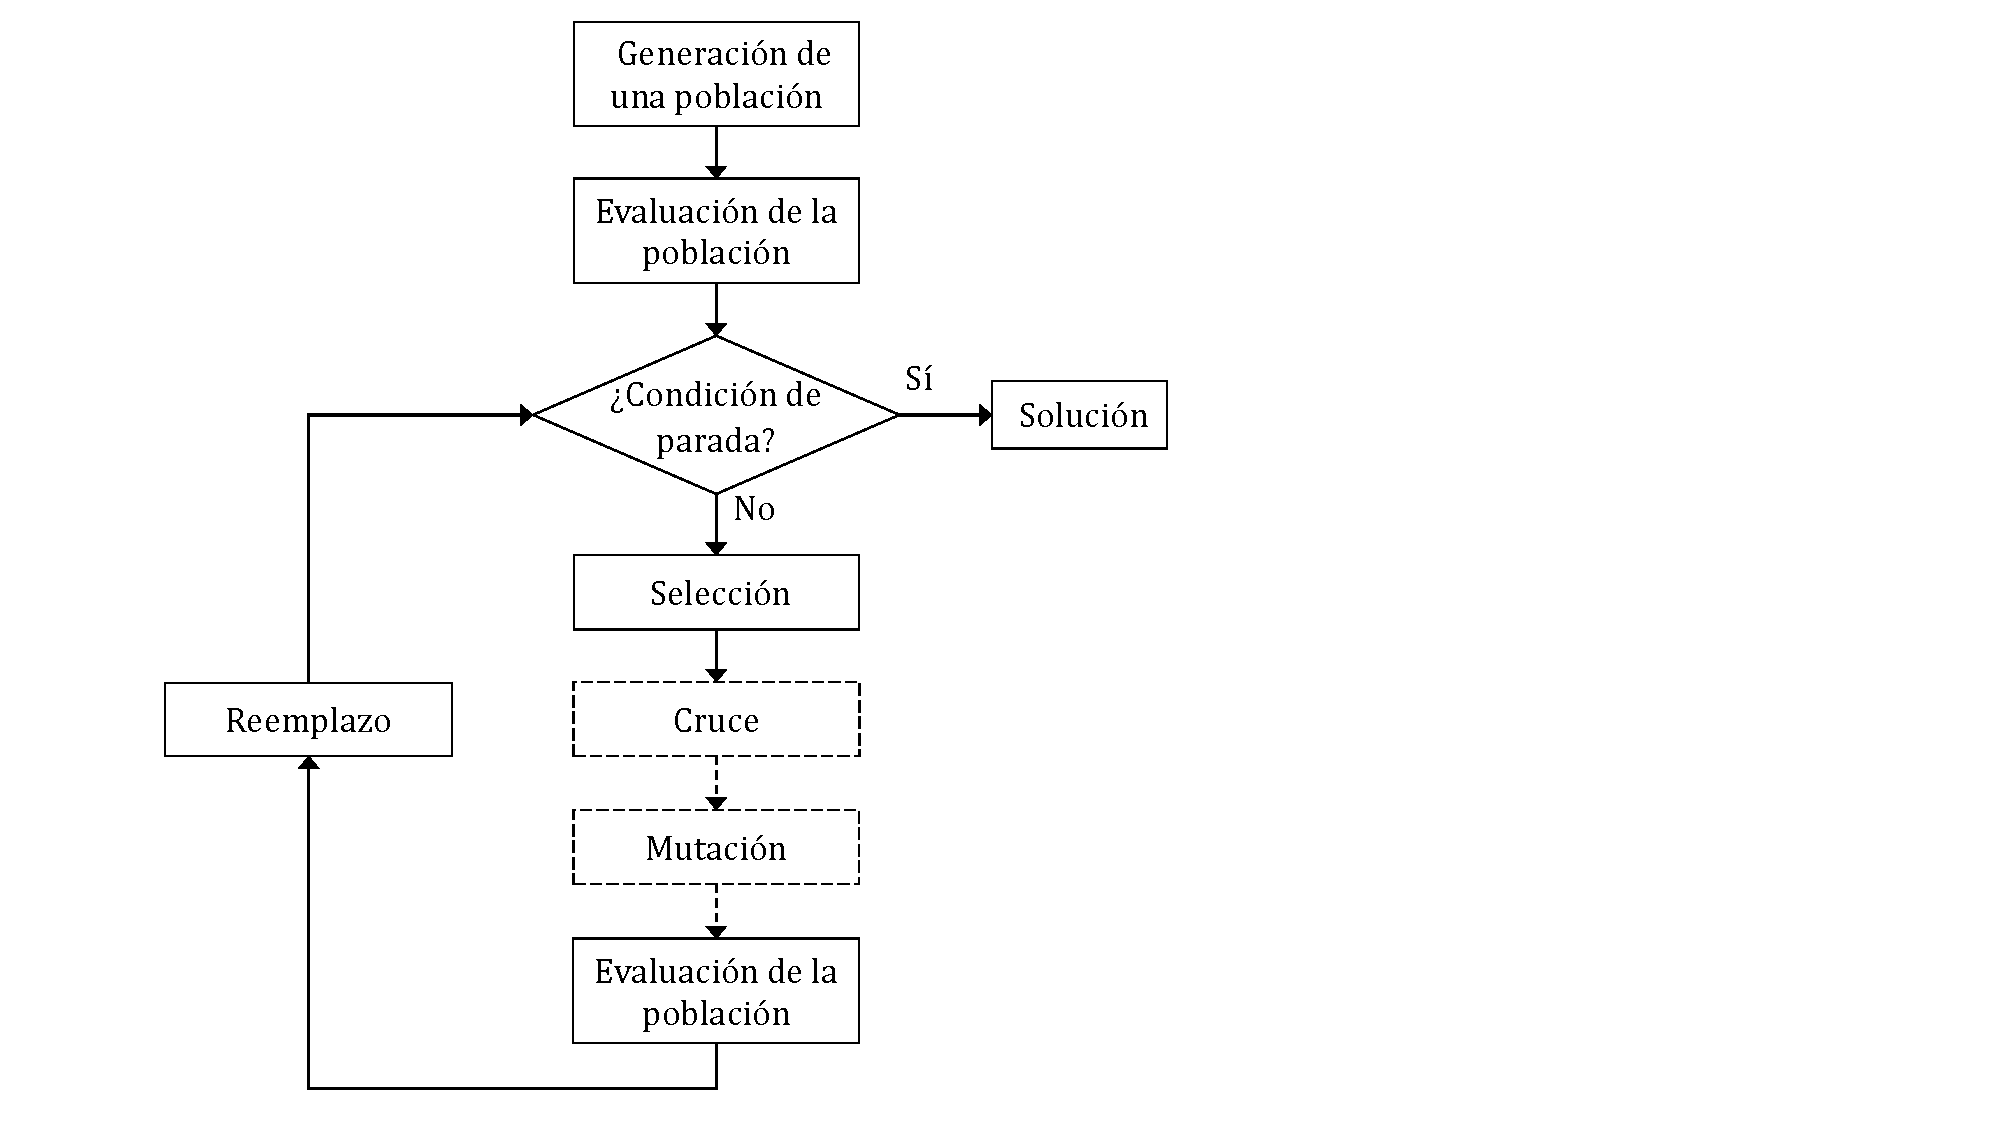
\includegraphics[width = 1.5\textwidth]{resources/Fig1.pdf}
    \caption{Ciclo Evolutivo que rige el desarrollo de los algoritmos en la Computación Evolutiva.}
    \label{fig:1}
  \end{figure}
  En la Fig. \ref{fig:1} se puede apreciar este Ciclo Evolutivo. Todo comienza con una población inicial, que se corresponde con un conjunto de individuos de tamaño $\alpha$ perteneciente a un espacio de búsqueda $E$, que codifica soluciones de un espacio $S$. Un individuo codifica una solución mediante un alfabeto $A$ y una función de codificación $\Omega$. La elección del alfabeto $A$ es fundamental, ya que de él depende que haya individuos del espacio $S$ que no tengan representación en el espacio $E$, y si es una solución potencialmente buena (incluyendo la óptima), entonces el proceso evolutivo nunca la encuentra. \par
  Tras la creación de la población inicial (a partir del espacio de búsqueda $E$), se evalúa, por medio de una función de evaluación (\emph{fitness function}), a sus individuos para determinar su grado de adaptación, es decir, la calidad de la solución que representa para el problema en cuestión. Para este proceso de evaluación, es necesario decodificar a los individuos, aplicando la función $\Omega$. \par
  Tras el proceso de generación de la población inicial y su evaluación, se determina si se cumple alguna condición de parada y en caso contrario, continúa. Algunas condiciones de parada pueden ser:
  \begin{enumerate}
    \item Algún individuo de la población representa la solución óptima al problema.
    \item La población ha convergido (a una solución óptima o no).
    \item Se ha alcanzado el número máximo de generaciones.
  \end{enumerate} \par
  En el primer caso, la ejecución finaliza devolviendo el individuo óptimo y, por tanto, encontrando la solución. Si la población converge sin haber encontrado antes un individuo óptimo, entonces finaliza devolviendo cualesquiera de los individuos de la misma. Si no se cumple ninguna de estas dos condiciones, entonces se comprueba si se han superado el número de generaciones máximas determinadas por el usuario. En caso afirmativo, finaliza devolviendo el mejor individuo de la población. En el caso de que no se cumpla ninguna condición de parada, el algoritmo continúa. \par
  Después se aplican los operadores genéticos de selección (\emph{selection}), cruce (\emph{crossover}) y mutación (\emph{mutation}) sobre los individuos. Tras aplicar estos tres operadores, se evalúan los nuevos individuos, se aplica el reemplazo y se comprueba si se cumple alguna condición de parada. El proceso se repite hasta que se cumpla alguna condición de parada. \par
  Los principales operadores genéticos son:
  \begin{itemize}
    \item Selección. Es el operador encargado de elegir a los individuos de la población que se van a cruzar para generar otros nuevos. El fundamento radica que en la naturaleza, aquellos individuos mejor adaptados tienen una probabilidad de reproducción mayor frente aquellos que no lo estén. Por tanto, una implementación tradicional consiste en seleccionar con mayor probabilidad a los mejor adaptados, pero hay otras elitistas que seleccionan solo a los $\pi$ mejor adaptados.
    \item Cruce. Los individuos seleccionados por el operador anterior acceden al \emph{mating pool}. Estos individuos reciben el nombre de progenitores (\emph{progenitors}), que se cruzan con cierta probabilidad para formar su descendencia (\emph{offspring}). Normalmente, los progenitores se cruzan por parejas, conformando 2 descendientes. Este operador se puede aplicar solo sobre los individuos seleccionados de la población y permite generar otros individuos nuevos. 
    \item Mutación. Con cierta probabilidad (normalmente muy baja), un individuo de la población experimenta cambios aleatorios en su genoma. Esto permite aumentar la diversidad de la población al generar otra posible solución potencial.
    \item Reemplazo. Este operador selecciona a los $\alpha$ individuos que formarán parte de la siguiente generación si no se cumple alguna condición de parada después de aplicar los operadores anteriores. Hay muchas políticas de reemplazo, pero el fin común es producir la mejora gradual de los individuos generación a generación y alcanzar la convergencia.
  \end{itemize} \par
  Se puede apreciar que los operadores genéticos resultan indispensables para el desarrollo y mejora de la población y su llegada hacia la solución óptima. En concreto, el cruce es el máximo responsable del proceso evolutivo, ya que es el encargado de generar nueva descendencia, tratando de seleccionar los mejores genes de cada progenitor. \par
  Según los operadores que se implementen, la técnica evolutiva tiende a explorar o explotar más el espacio de búsqueda. La exploración consiste en muestrear regiones desconocidas en el espacio de búsqueda donde pueden encontrarse las soluciones óptimas. La explotación trata de mejorar al individuo más destacado, acortando la búsqueda de la solución óptima en una búsqueda local. Por tanto, estos operadores (y en especial el operador de cruce) se deben comportar de forma explotativa en las primeras generaciones, ya que hay una gran diversidad y de otra forma se produce una convergencia muy lenta. Sin embargo, a medida que la población va convergiendo hacia una solución, es necesario que los operadores exploren, es decir, tengan la posibilidad de dirigirse hacia otras regiones de búsqueda para evitar la caida en óptimos no globales. \par
  
  \section*{\Large 2.3. Programación Genética}
  La Programación Genética (Cramer, 1985; Koza, 1988) es una heurística de la familia de la Computación Evolutiva que permite resolver problemas de búsqueda y optimización cuya solución es un programa informático. La Programación Genética es similar a los Algoritmos Genéticos (Holland, 1967), donde el espacio de soluciones está compuesto por programas informáticos.
    \subsection*{\large 2.3.1. Codificación y representación de los individuos}
    Los individuos en la Programación Genética se representan mediante árboles, formados por operadores o funciones y operandos. Los operadores son los nodos intermedios, mientras que los operandos son los nodos hoja. Esta representación permite la codificación de programas informáticos. En la Fig. \ref{fig:2} se ejemplifican dos individuos en forma de árbol y su codificación. \par
    La creación de los individuos debe cumplir dos propiedades. La primera de ellas se refiere a la propiedad del cierre (\emph{closure property}), que evita la creación de individuos sintácticamente no válidos, estableciendo que la salida de una función debe poder servir de entrada para otra. La segunda propiedad es la explosión de código (\emph{code bloat}) (Tackett, 1995), que recoge el crecimiento desmesurado del código sin mejora de la adaptación, y, por lo tanto, debe evitarse en la medida de lo posible. La explosión de código propicia el aparecimiento de intrones (\emph{introns}), que son fragmentos de código totalmente inútiles y que no favorecen la adaptación y que se traduce en una convergencia lenta y una demora en la evaluación de los individuos. El alfabeto $A$ y la función de codificación $\Omega$ debe buscar en la medida de lo posible la biyección entre el espacio de soluciones y el espacio de búsqueda y que sea completo, es decir, que se puedan codificar todas las soluciones. \par
    \begin{figure}[H]
      \centering
      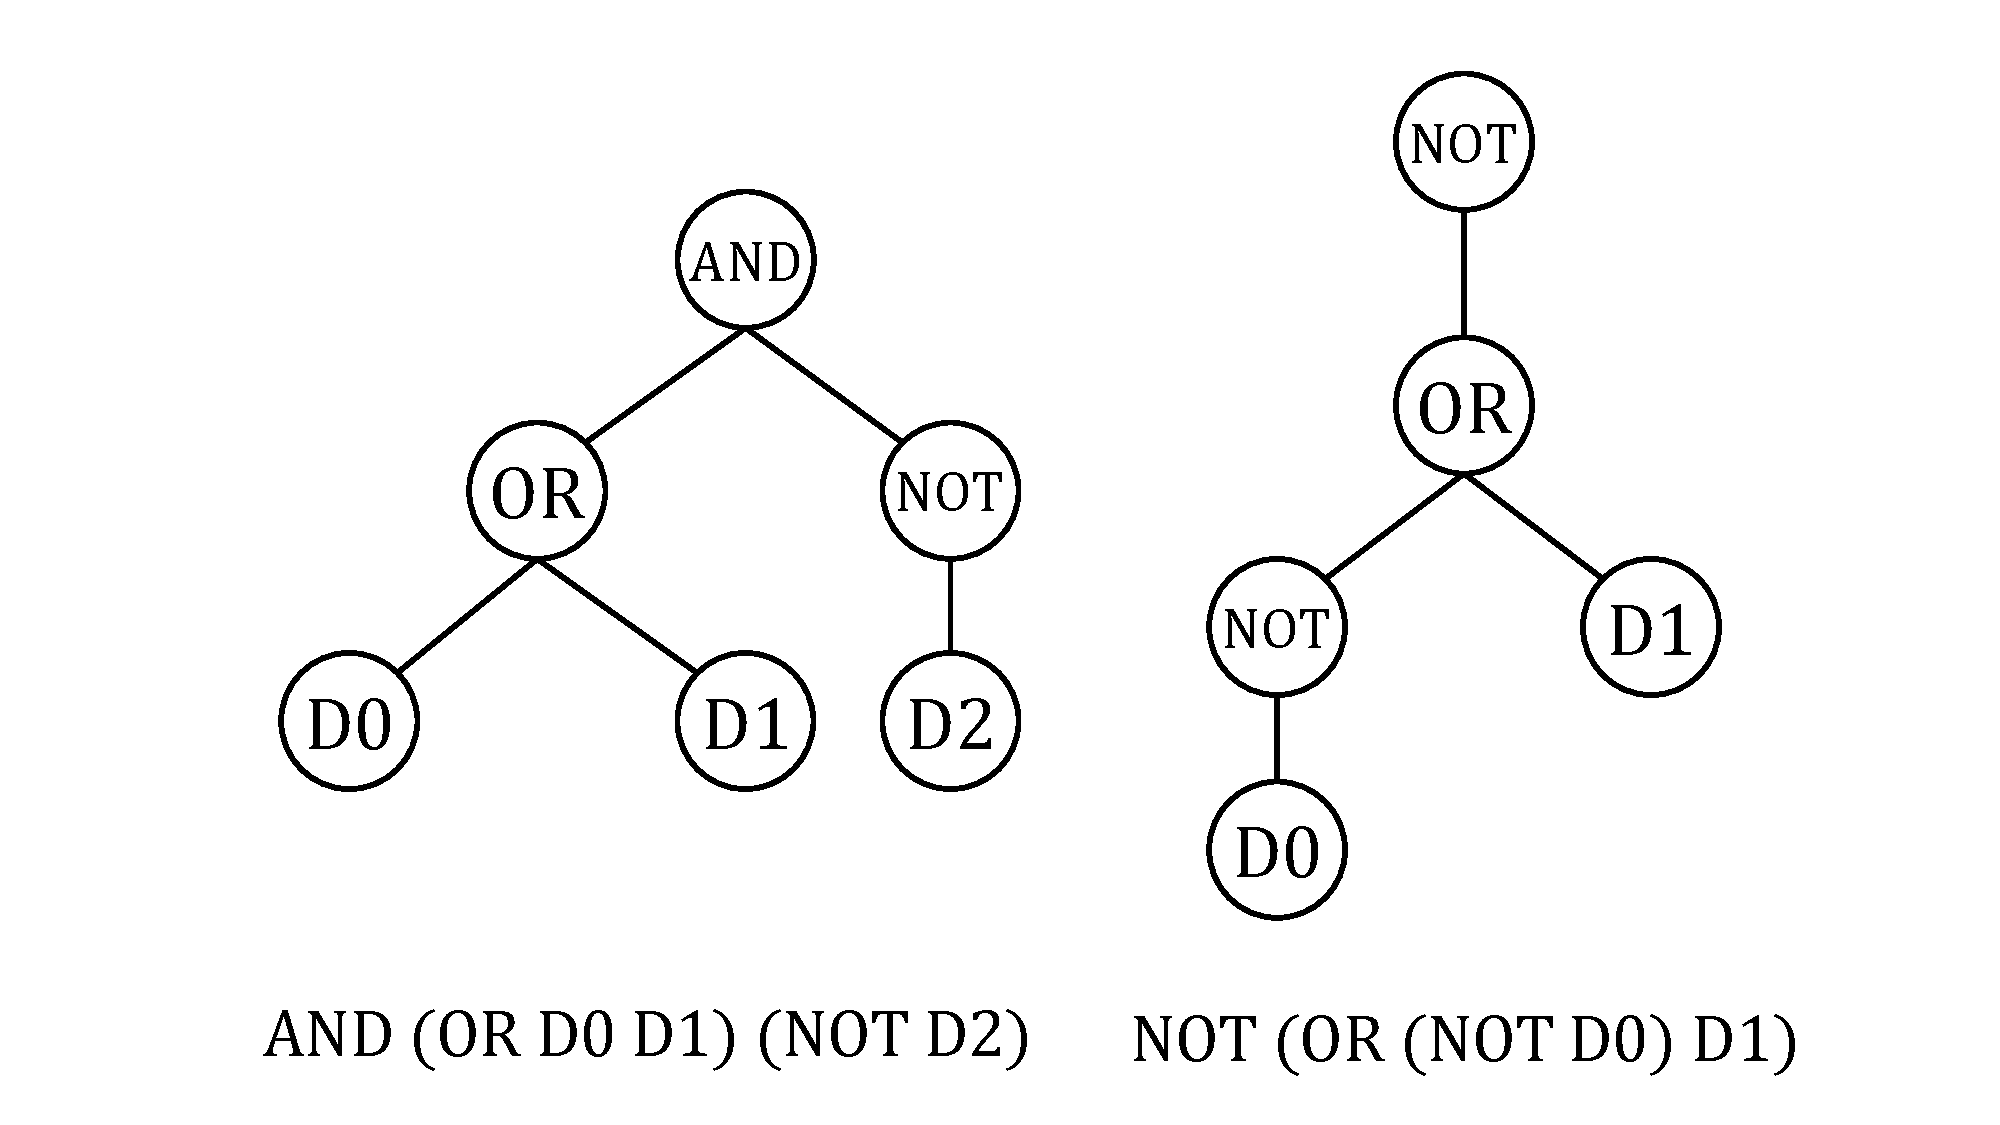
\includegraphics[width = 0.7\textwidth]{resources/Fig2.pdf}
      \caption{Individuos de un programa genético codificados en forma de árbol y su correspondiente decodificación.}
      \label{fig:2}
    \end{figure} \par
  
    \subsection*{\large 2.3.2. Generación de la población inicial}
    El programa genético debe partir de una población de individuos inicial, que es un subconjunto del espacio de búsqueda. La metodología de creación de individuos en Programación Genética suele ser aleatoria. \par
    Si se generan individuos de forma aleatoria, hay una gran probabilidad de que no se cumpla la propiedad del cierre y que haya explosión de código. Por tanto, es necesario un proceso de reparación de individuos. Normalmente, se basan en la sustitución de nodos mal colocados por otros correctos de forma aleatoria, como se muestra en la Fig. \ref{fig:5}. \par
    Este proceso de reparación muchas veces es más lento que la generación de un nuevo individuo, por lo que en la práctica los individuos inválidos se descartan y se sustituyen por otros, que si son nuevamente no válidos se descartan, repitiendo ese proceso hasta que se alcanza una población del tamaño deseado, con todos sus individuos siendo sintácticamente válidos.
    \begin{figure}[H]
      \centering
      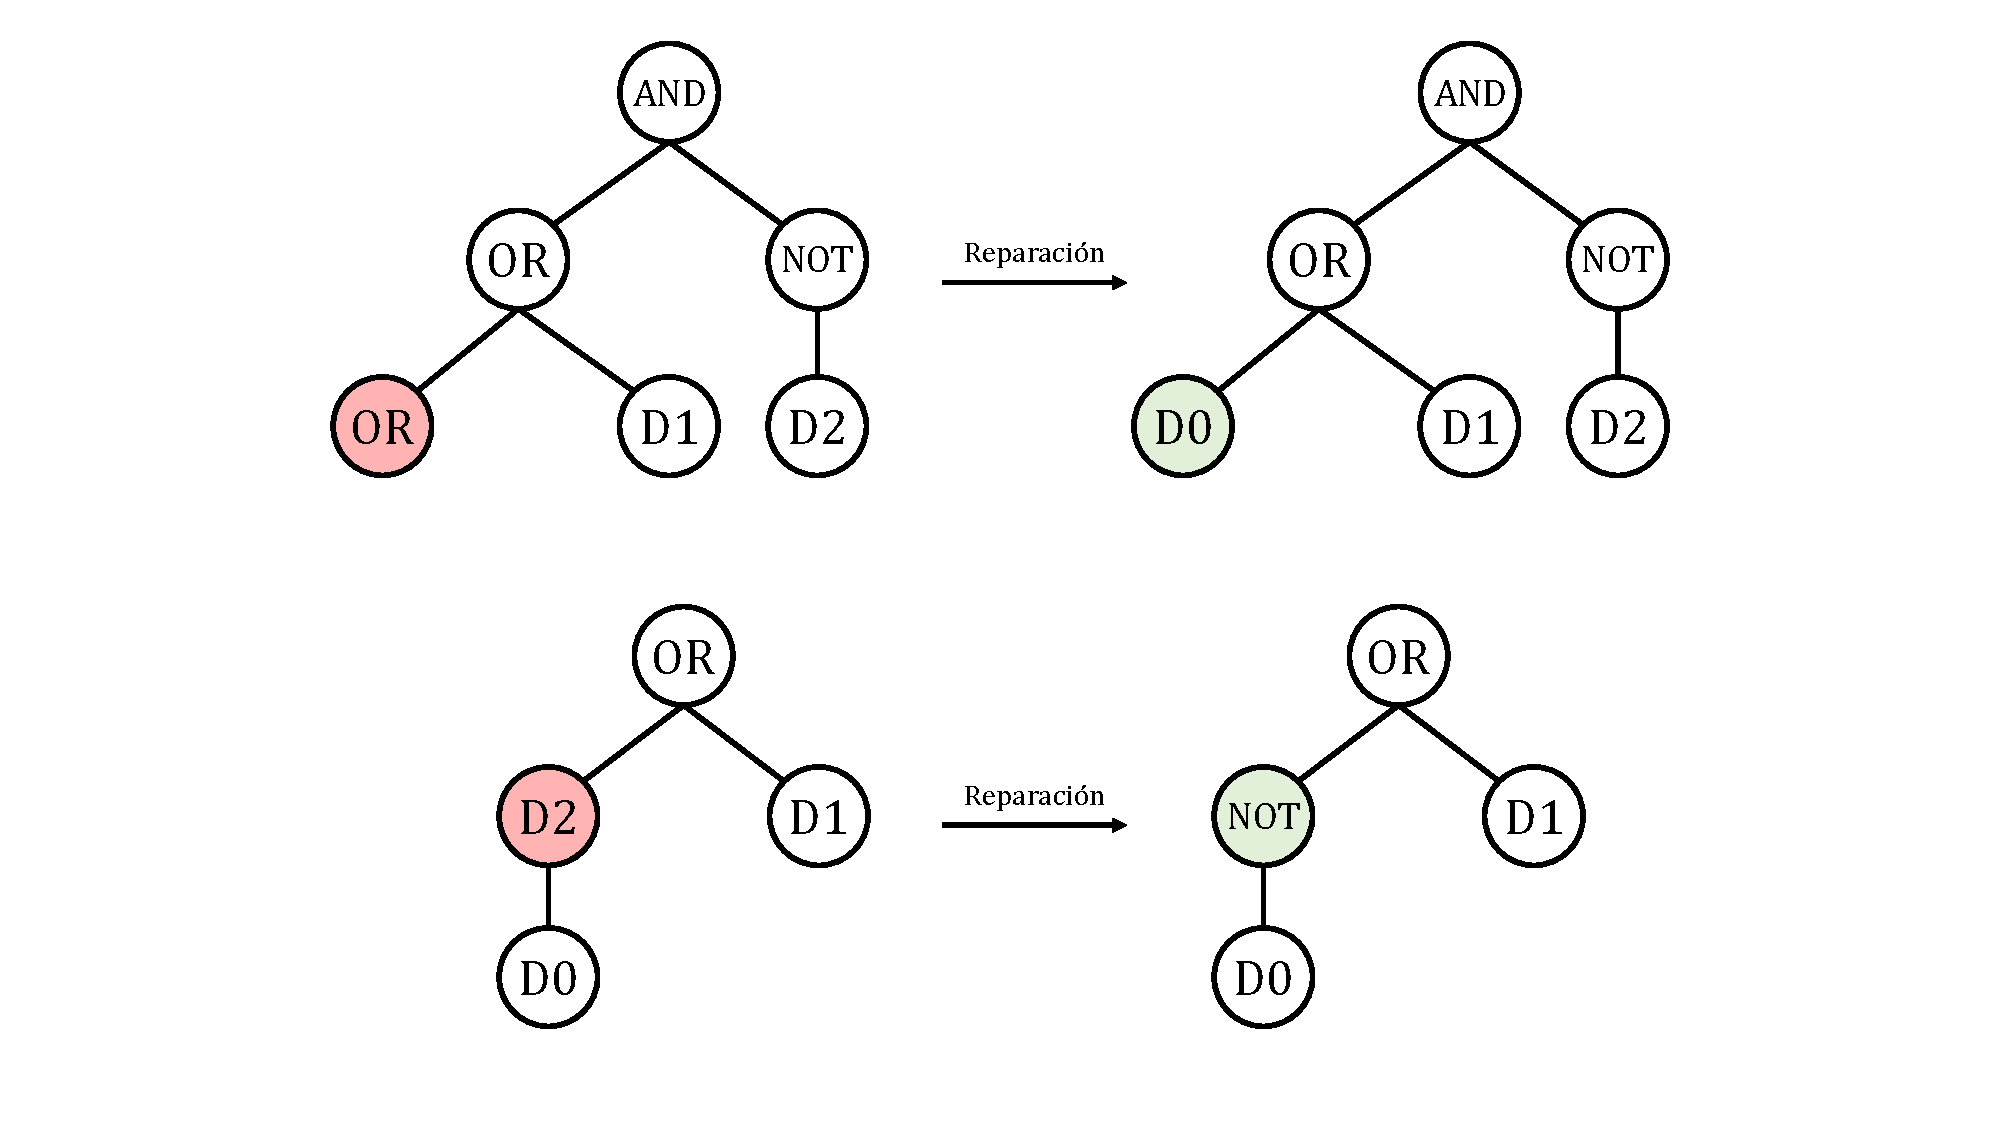
\includegraphics[width = 1\textwidth]{resources/Fig5.pdf}
      \caption{Ejemplo de aplicación de la función de reparación de individuos inválidos.}
      \label{fig:5}
    \end{figure} \par
  
    \subsection*{\large 2.3.3. Operadores}
    La Programación Genética cuenta con cuatro operadores: selección, cruce, mutación y reemplazo. Aquellos que no modifican a los individuos son el de selección y el de reemplazo, por lo que funcionan de forma análoga a como hacen en otras heurísticas como en los Algoritmos Genéticos o en la Evolución Gramatical, por lo que solo se explica el operador de cruce y el de mutación.
    
      \subsubsection*{\normalsize 2.3.2.1. Cruce}
      El operador de cruce se aplica con cierta probabilidad sobre los individuos que han sido seleccionados y que se encuentran en el mating pool, por tanto, no se aplica en todos los individuos. El cruce debe asegurar que se cumple la propiedad del cierre y que no haya explosión de código. \par
      
        \subsubsection*{\vspace{-0.5cm}{\normalsize Operador de Koza}}
        \vspace{-0.5cm}
        El operador de cruce de Koza (Koza, 1992) selecciona un nodo de cada padre de forma aleatoria y se intercambian los subárboles. Este operador no asegura que se cumpla la propiedad del cierre, además, como en el ejemplo mostrado en la Fig. \ref{fig:3}, se corre el riesgo de que se produzcan intrones como consecuencia de la explosión de código, ya que no cuenta con un mecanismo de control de profundidad. \vfill
        \begin{figure}[H]
          \centering
          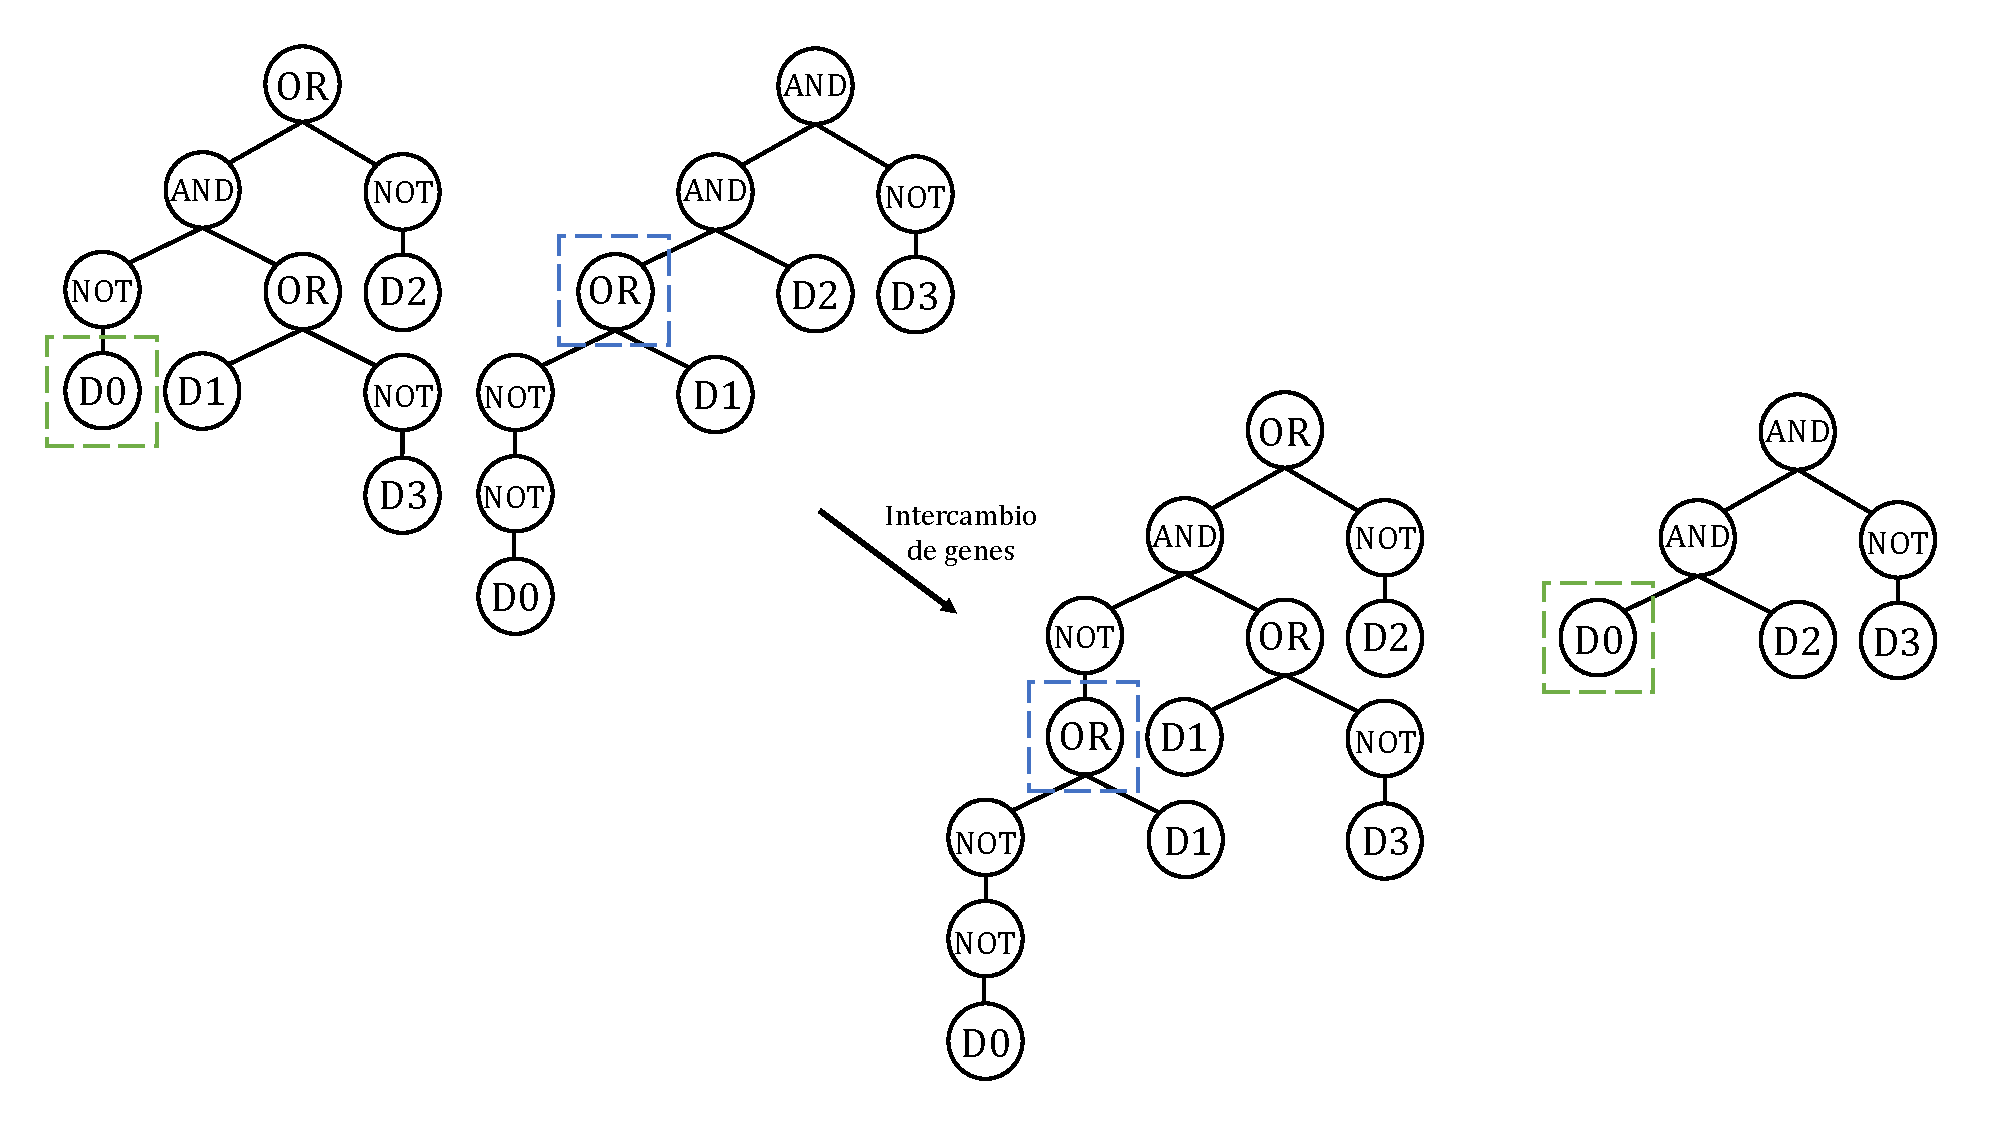
\includegraphics[width = 1\textwidth]{resources/Fig3.pdf}
          \caption{Ejemplo de aplicación del operador de cruce de Koza.}
          \label{fig:3}
        \end{figure} \par
        
        \subsubsection*{\vspace{-0.5cm}{\normalsize Operador basado en un punto}}
        \vspace{-0.5cm}
        El operador de cruce basado en un punto (Poli and Langdon, 1997a, 1997b, 1998) de la Programación Genética se inspira en el de los Algoritmos Genéticos (Goldberg, 1989). Este operador selecciona el nodo de cruce después de un proceso de alineamiento (\emph{alignment}) entre los padres, donde se seleccionan los nodos potenciales para realizar el intercambio.
        \begin{figure}[H]
          \centering
          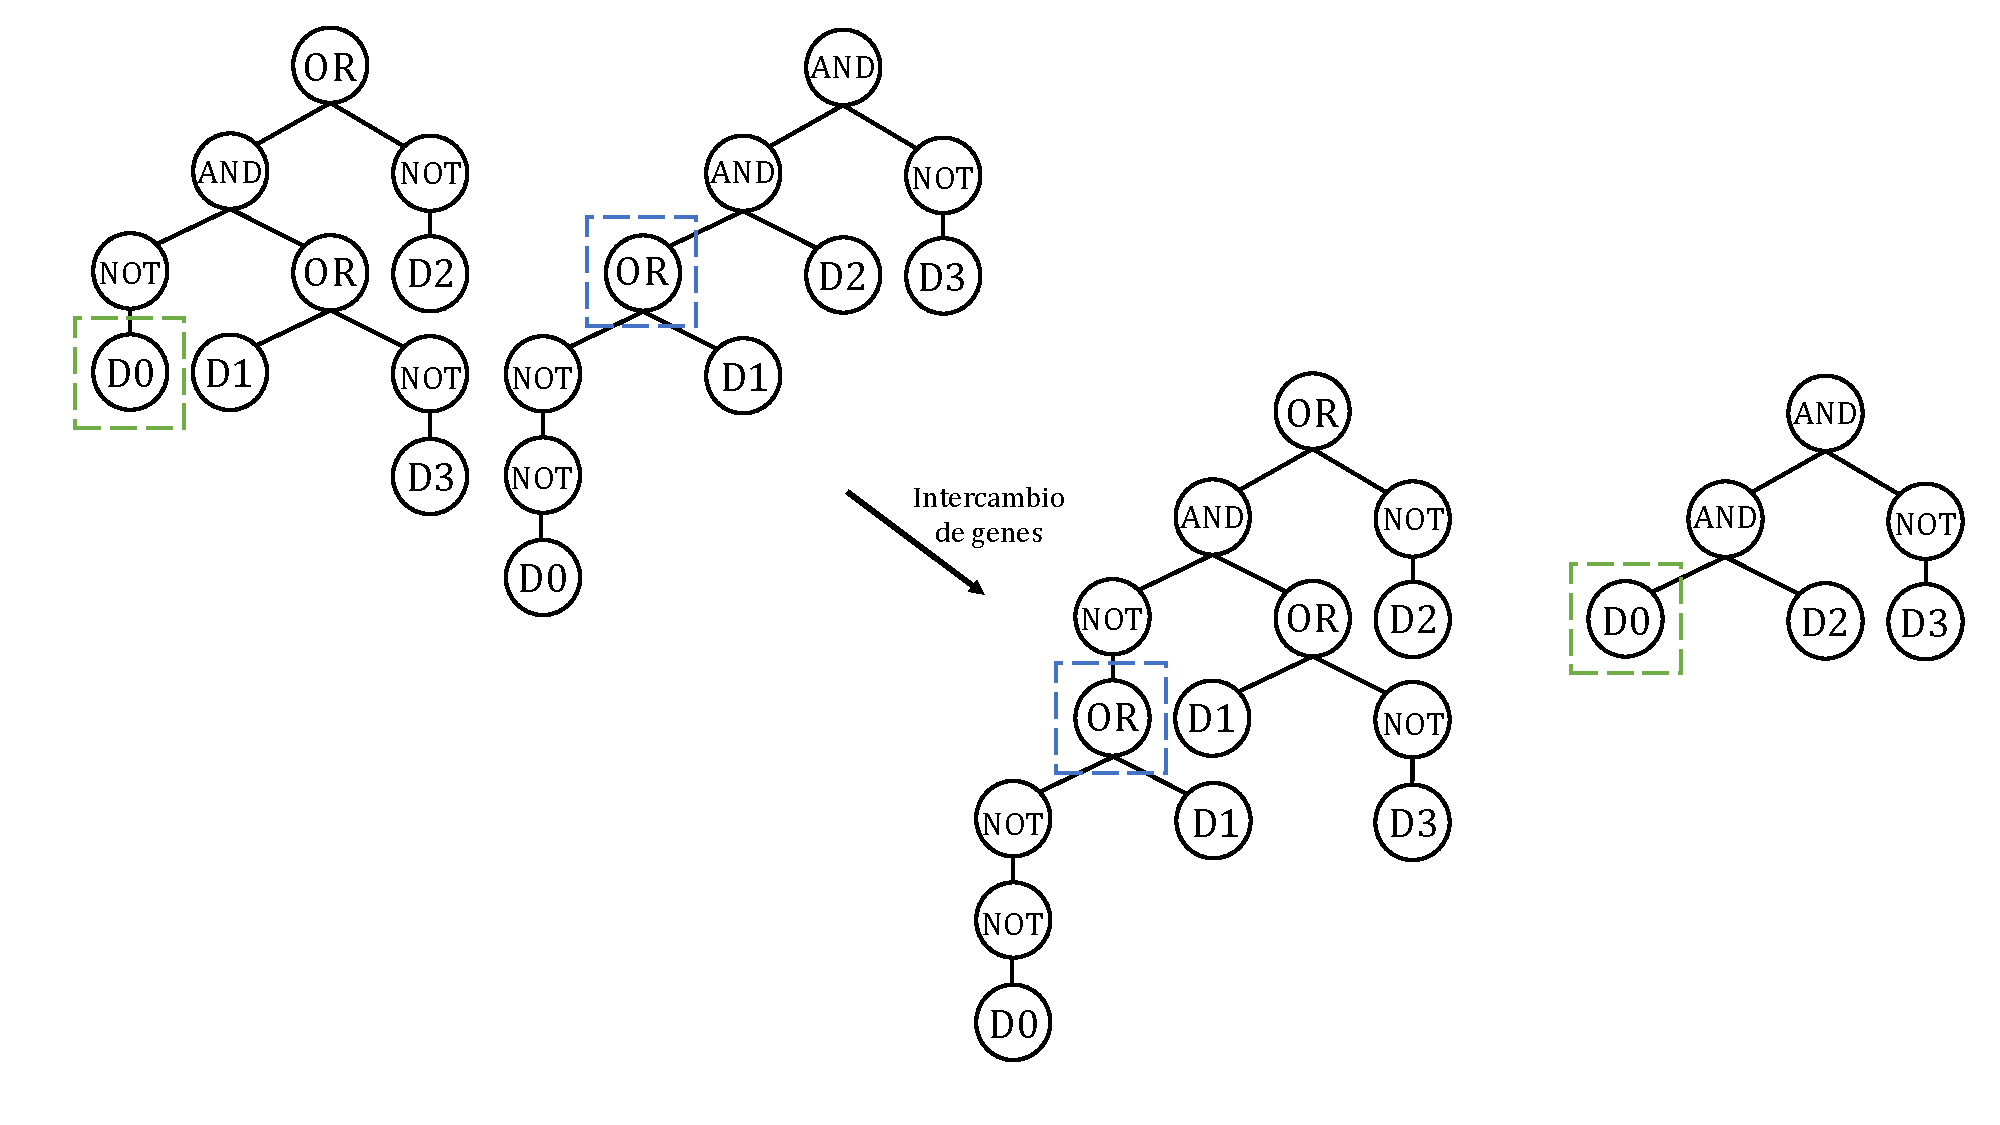
\includegraphics[width = 1\textwidth]{resources/Fig4.pdf}
          \caption{Ejemplo de aplicación del operador de cruce basado en un punto.}
          \label{fig:4}
        \end{figure} \par
        Este operador selecciona un nodo de forma aleatoria de entre los coincidentes entre los dos padres. El problema que tiene este operador es que si la estructura de los padres es totalmente distinta, entonces el único símbolo coincidente entre los padres será el símbolo raíz, produciendo entonces una descendencia idéntica a los progenitores, por lo que se puede dar una convergencia prematura a un óptimo local.
        
      \subsubsection*{\normalsize 2.3.2.2. Mutación}
      El operador de mutación se aplica con una muy baja probabilidad a los individuos seleccionados y a su descendencia. Debido a la baja probabilidad, puede que haya generaciones en las que no haya mutación. De hecho, hay programas genéticos que no utilizan este operador. Este operador selecciona un nodo de forma aleatoria en el individuo seleccionado, y a continuación, genera un subárbol a partir de ese nodo seleccionado de forma análoga a como se inicializan las poblaciones.

  \section*{\Large 2.4. Programación Genética Guiada por Gramáticas}
  La Programación Genética Guiada por Gramáticas (Whigham, 1995) surge por las dificultades encontradas en el desarrollo de los programas genéticos en relación con la propiedad del cierre. En concreto, la aleatoriedad en la creación de individuos resulta una dificultad cuando los problemas son grandes y la cantidad de símbolos es elevada, pues hay más probabilidades de generar un individuo no válido (Vanneschi et al., 2010). Además, la función de reparación o la sustitución de individuos no válidos por otros bien formados aumenta la complejidad computacional. \par
  La Programación Genética Guiada por Gramáticas evita los problemas de la creación de individuos no válidos gracias a la utilización de Gramáticas Libres de Contexto (\emph{context-free grammars}) (Chomsky, 1959), que permiten que las soluciones que codifican los individuos formen parte del espacio de soluciones aunque sean generados de forma aleatoria.
  
    \subsection*{\large 2.4.1. Gramáticas Libres de Contexto}
    Una Gramática Libre de Contexto $G$ está definida por una 4-tupla (Hopcroft and Ullman, 1979) de la forma: 
    \begin{align}
    G = (\Sigma_{N}, \Sigma_{T}, S, P), \label{eq:1}\tag{1}
    \end{align}
    donde $\Sigma_{N}$ se corresponde con el conjunto de símbolos no terminales (variables), $\Sigma_{T}$ con el conjunto de símbolos terminales (constantes), $S$ es el axioma o símbolo inicial, del que derivan las reglas que forman al individuo y $P$ es el conjunto de reglas de producción. \par
    Una regla de producción (\emph{production rule}) de $P$ tienen la forma $\alpha \rightarrow \beta$, donde $\alpha$ es un símbolo no terminal, $\alpha \in \Sigma_{N}$, y $\beta$ es una cadena de variables o terminales con $\beta \in (\Sigma_{N} \cup \Sigma_{T})^*$. \par
    Una derivación de la gramática $G$ es un conjunto de reglas de producción $\alpha \rightarrow^*s$, $s \in \Sigma_{T}^*$, donde $s$ es palabra, que se corresponde con la decodificación del individuo en el espacio de soluciones. \par
    La Programación Genética Guiada por Gramáticas asegura que los individuos generados son siempre válidos porque siguen la sintaxis definida en la gramática. Sin embargo, pueden existir reglas de producción recursivas, por lo que puede haber explosión de código. \par
    Otra característica de estas gramáticas es que puede haber ambigüedad, es decir, puede haber dos individuos distintos pero que deriven la misma palabra. Por ejemplo, la siguiente gramática es ambigua: \\
    \begin{align*}
    G &= (\Sigma_{N}, \Sigma_{T}, S, P) \label{eq:2}\tag{2} \\
    \Sigma_{N} &= \{S, E, F, N\} \\
    \Sigma_{T} &= \{0, 1, 2, 3, 4, 5, 6, 7, 8, 9, +, -, =\} \\
    P &= \{ \\
    &S ::= E = N \\
    &E ::= E + E | E - E | F + E | F - E | N \\
    &F ::= N \\
    &N ::= 0 | 1 | 2 | 3 | 4 | 5 | 6 | 7 | 8 | 9 \\
    \}
    \end{align*} \par
    \begin{figure}[H]
      \centering
      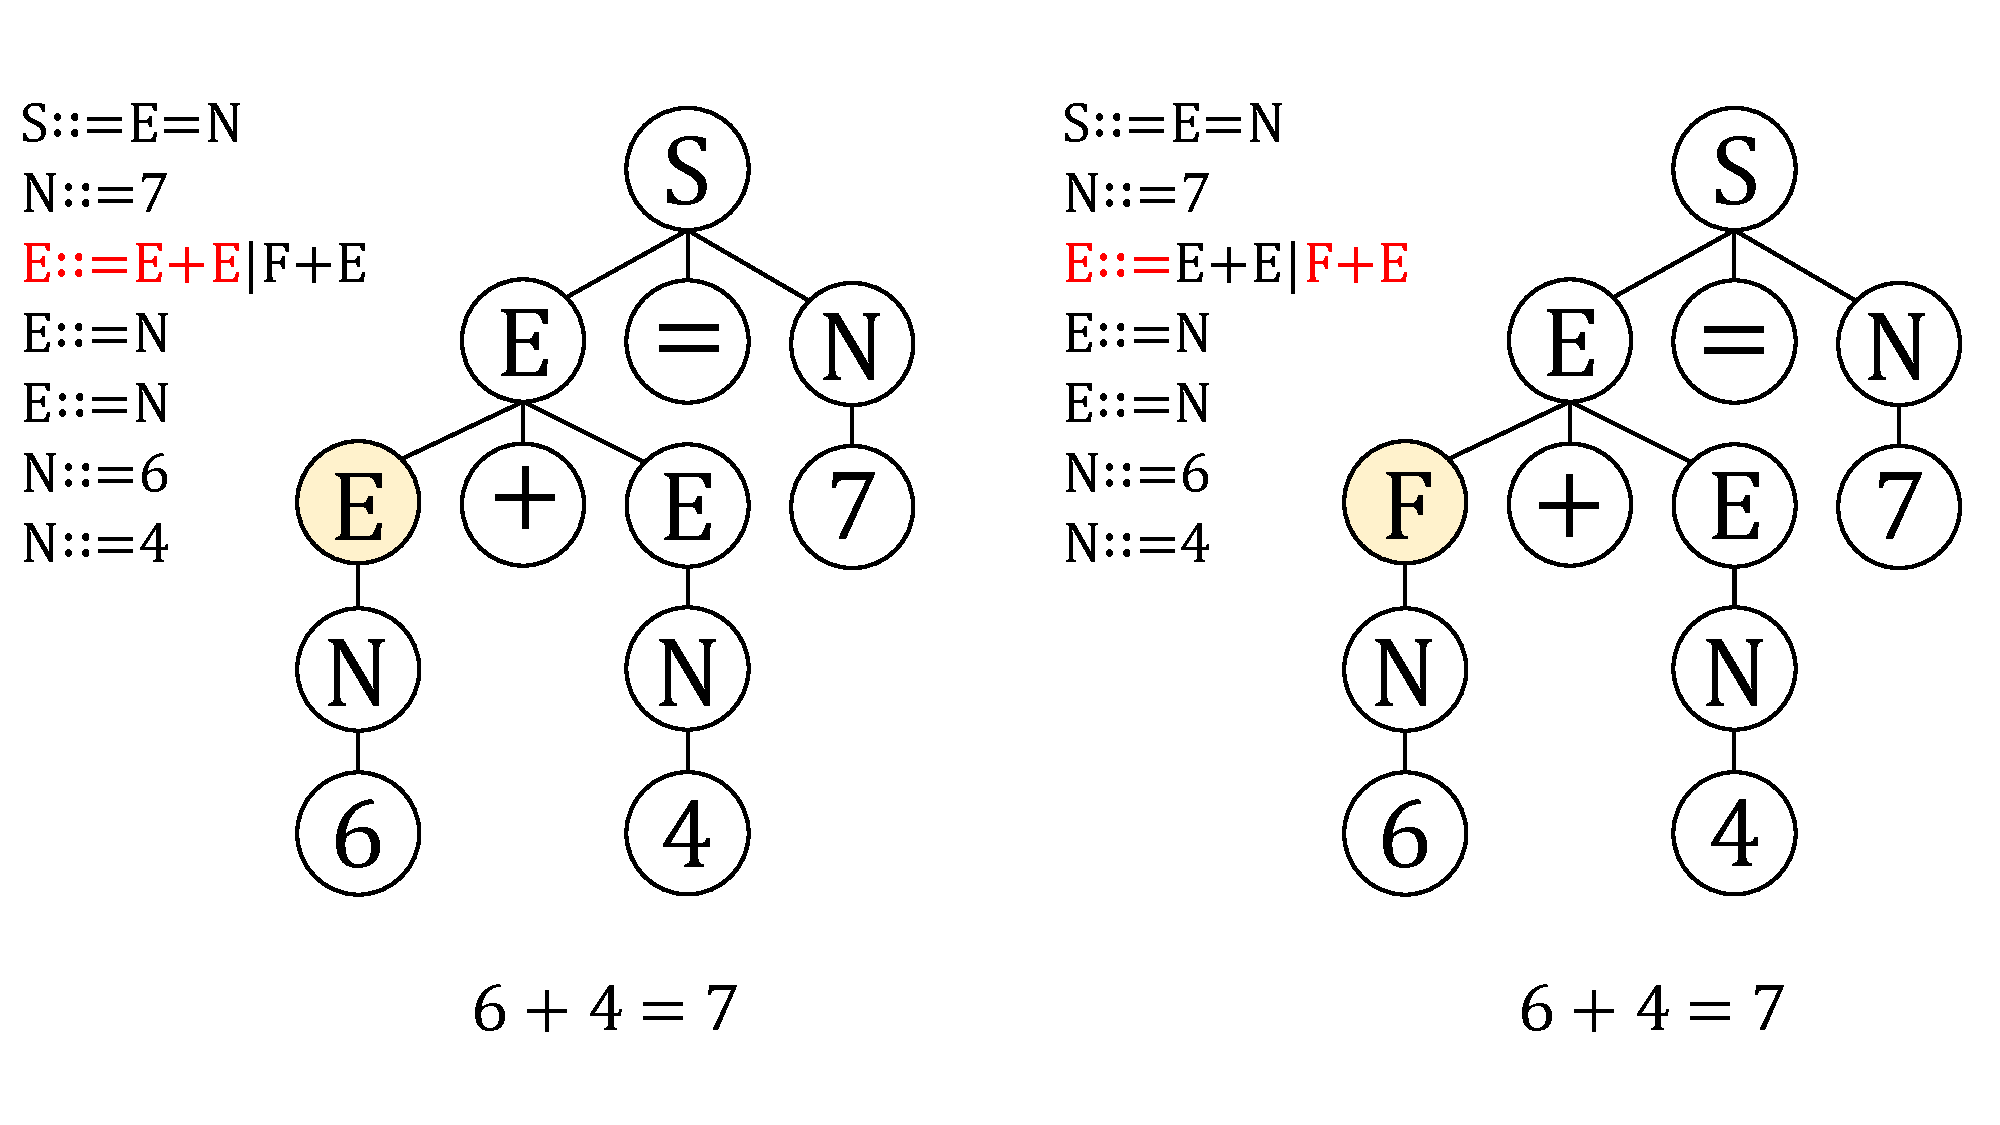
\includegraphics[width = 0.8\textwidth]{resources/Fig6.pdf}
      \caption{Individuos conformados por una gramática redundante.}
      \label{fig:6}
    \end{figure} \par
    La Fig. \ref{fig:6} muestra dos individuos diferentes que representan la misma palabra. Se puede comprobar que los símbolos no terminales $F$ y $E$ son equivalentes, ya que de ellos derivan reglas idénticas. \par
    
    \subsection*{\large 2.4.2. Codificación y representación de los individuos}
    Los individuos son árboles de derivación. Estos árboles son creados empleando una Gramática Libre de Contexto. La decodificación de estos individuos se obtiene leyendo los nodos terminales de izquierda a derecha, sin incluir los nodos interiores. \par
    Una gramática es recursiva cuando tiene producciones recursivas. Por ejemplo, la gramática mostrada en la Eq. \ref{eq:2} es recursiva, ya que tres de las cuatro producciones del nodo no terminal $E$ son recursivas. En tal caso, dependiendo del algoritmo de generación de individuos que se utilice, se pueden producir o no intrones. 
    
    \subsection*{\large 2.4.3. Generación de la población inicial}
    Para la creación de individuos para la población inicial, hay dos técnicas: una aleatoria y otra controlada. La primera de ellas, utiliza la Gramática Libre de Contexto y genera derivaciones de forma aleatoria, siguiendo las reglas de producción. A pesar de que genera individuos sintácticamente válidos y es simple de aplicar, es incapaz de controlar la profundidad, facilitando la aparición de la explosión de código. \par
    El segundo método es una variante del primero, ya que los individuos también se generan de forma aleatoria, pero controlando en todo momento la profundidad de la derivación, no permitiendo en ningún caso que se sobrepase la profundidad máxima. Para ello, el algoritmo conoce en todo momento la profundidad actual del individuo que está generando y busca reglas de producción que mantengan la profundidad del individuo dentro del límite de profundidad (García-Arnau et al., 2007).
    
    \subsection*{\large 2.4.4. Operadores}
    Los operadores de la Programación Genética de cruce y mutación son también útiles en la Programación Genética Guiada por Gramáticas, al igual que los operadores comunes de selección y de reemplazo. Con la adición de las gramáticas, existen varias implementaciones nuevas sobre el operador de cruce.
    
      \vspace{-0.5cm}
      \subsubsection*{\normalsize 2.4.3.1. Cruce}
      Si bien los operadores de cruce de la Programación Genética pueden utilizarse en la Programación Genética Guiada por Gramáticas, los individuos generados con ellos pueden ser no válidos y no cumplirán, por tanto, con la propiedad de cierre. El ejemplo más evidente se hace palpable con el operador de cruce de Koza (Koza, 1992), que genera puntos de cruce de forma aleatoria y que no tiene en cuenta las reglas de producción, tal y como se muestra en la Fig. \ref{fig:7} con la gramática mostrada en la Eq. \ref{eq:2}. \par
      \begin{figure}[H]
        \centering
        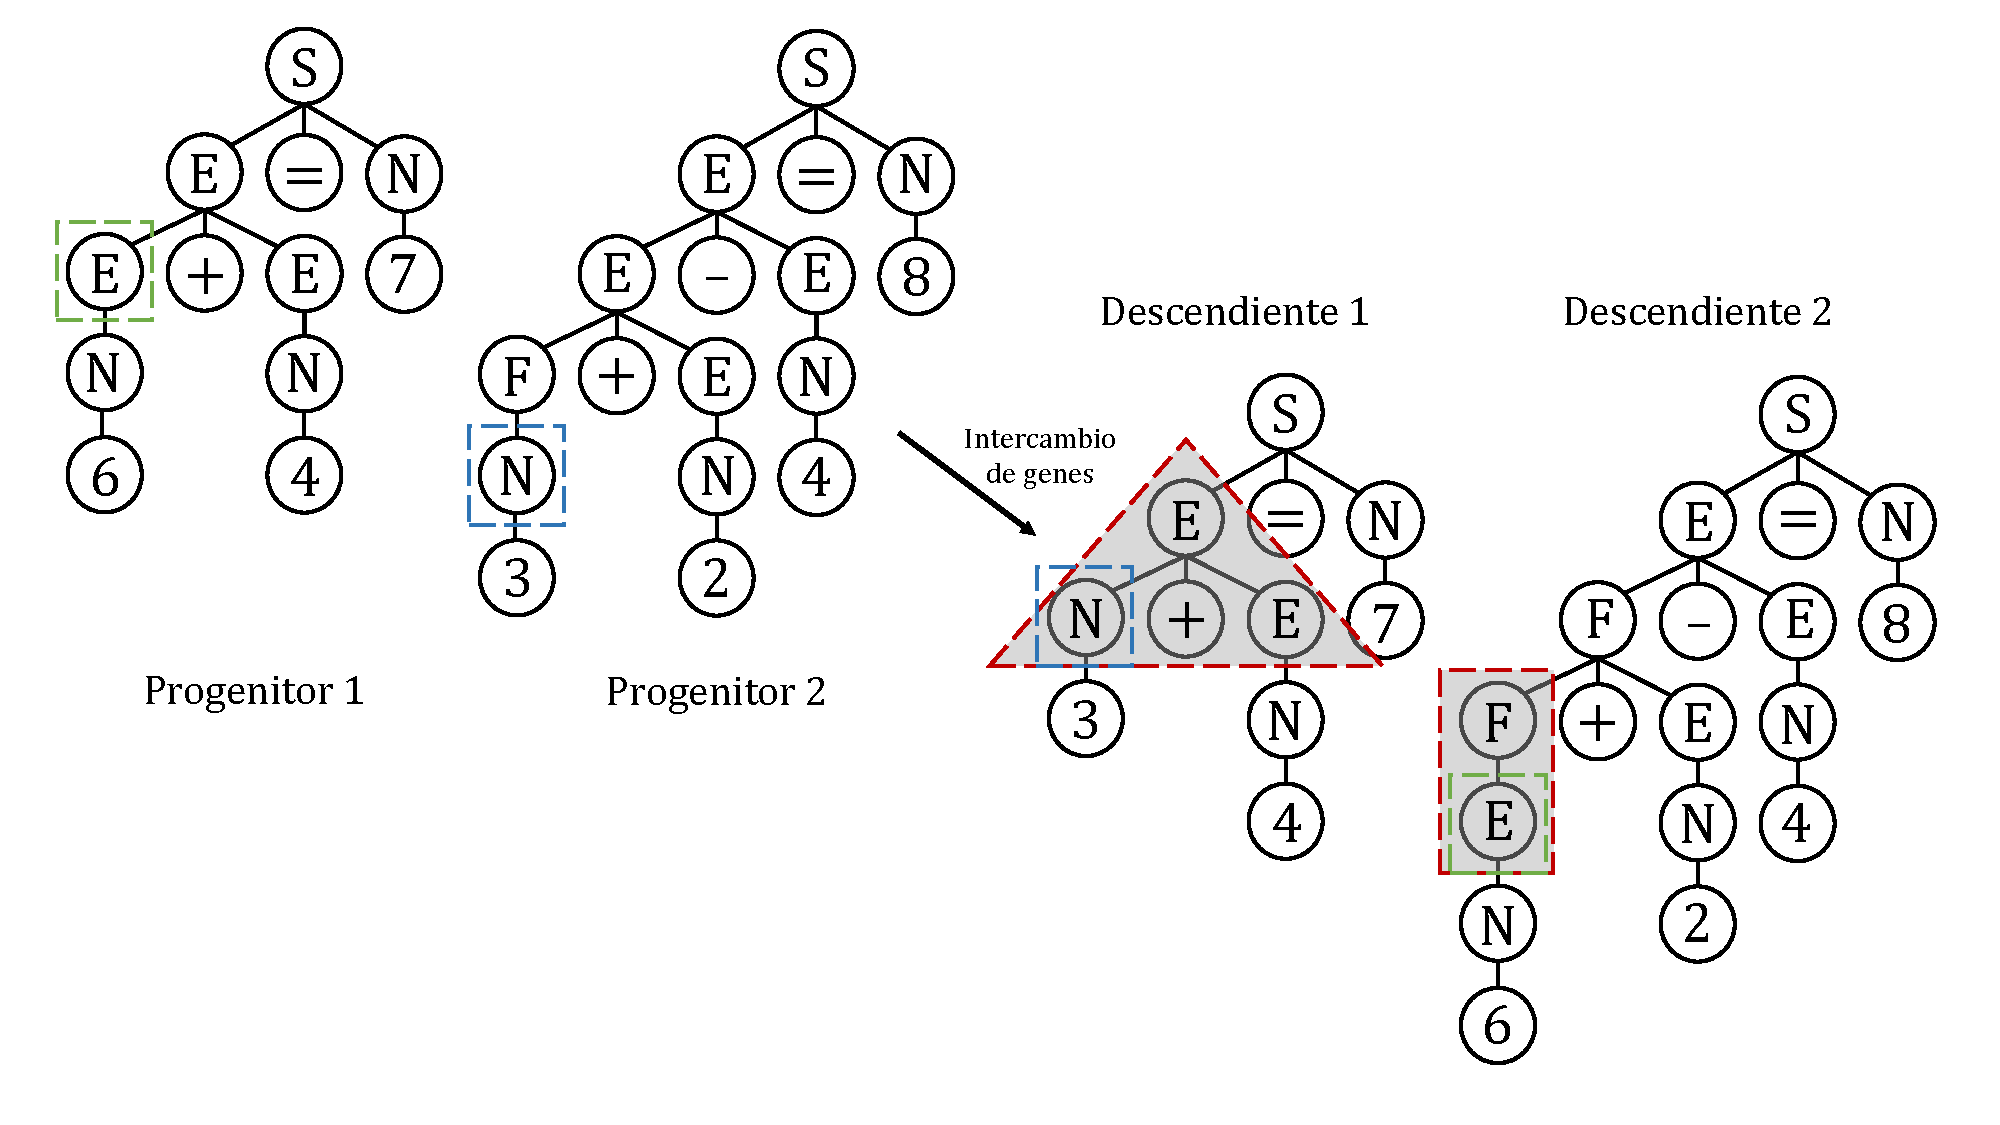
\includegraphics[width = 1\textwidth]{resources/Fig7.pdf}
        \caption{Errores (en rojo) producidos en el cruce de dos individuos generados con gramáticas al aplicar el operador de Koza.}
        \label{fig:7}
      \end{figure} 
        \begin{figure}[H]
          \centering
          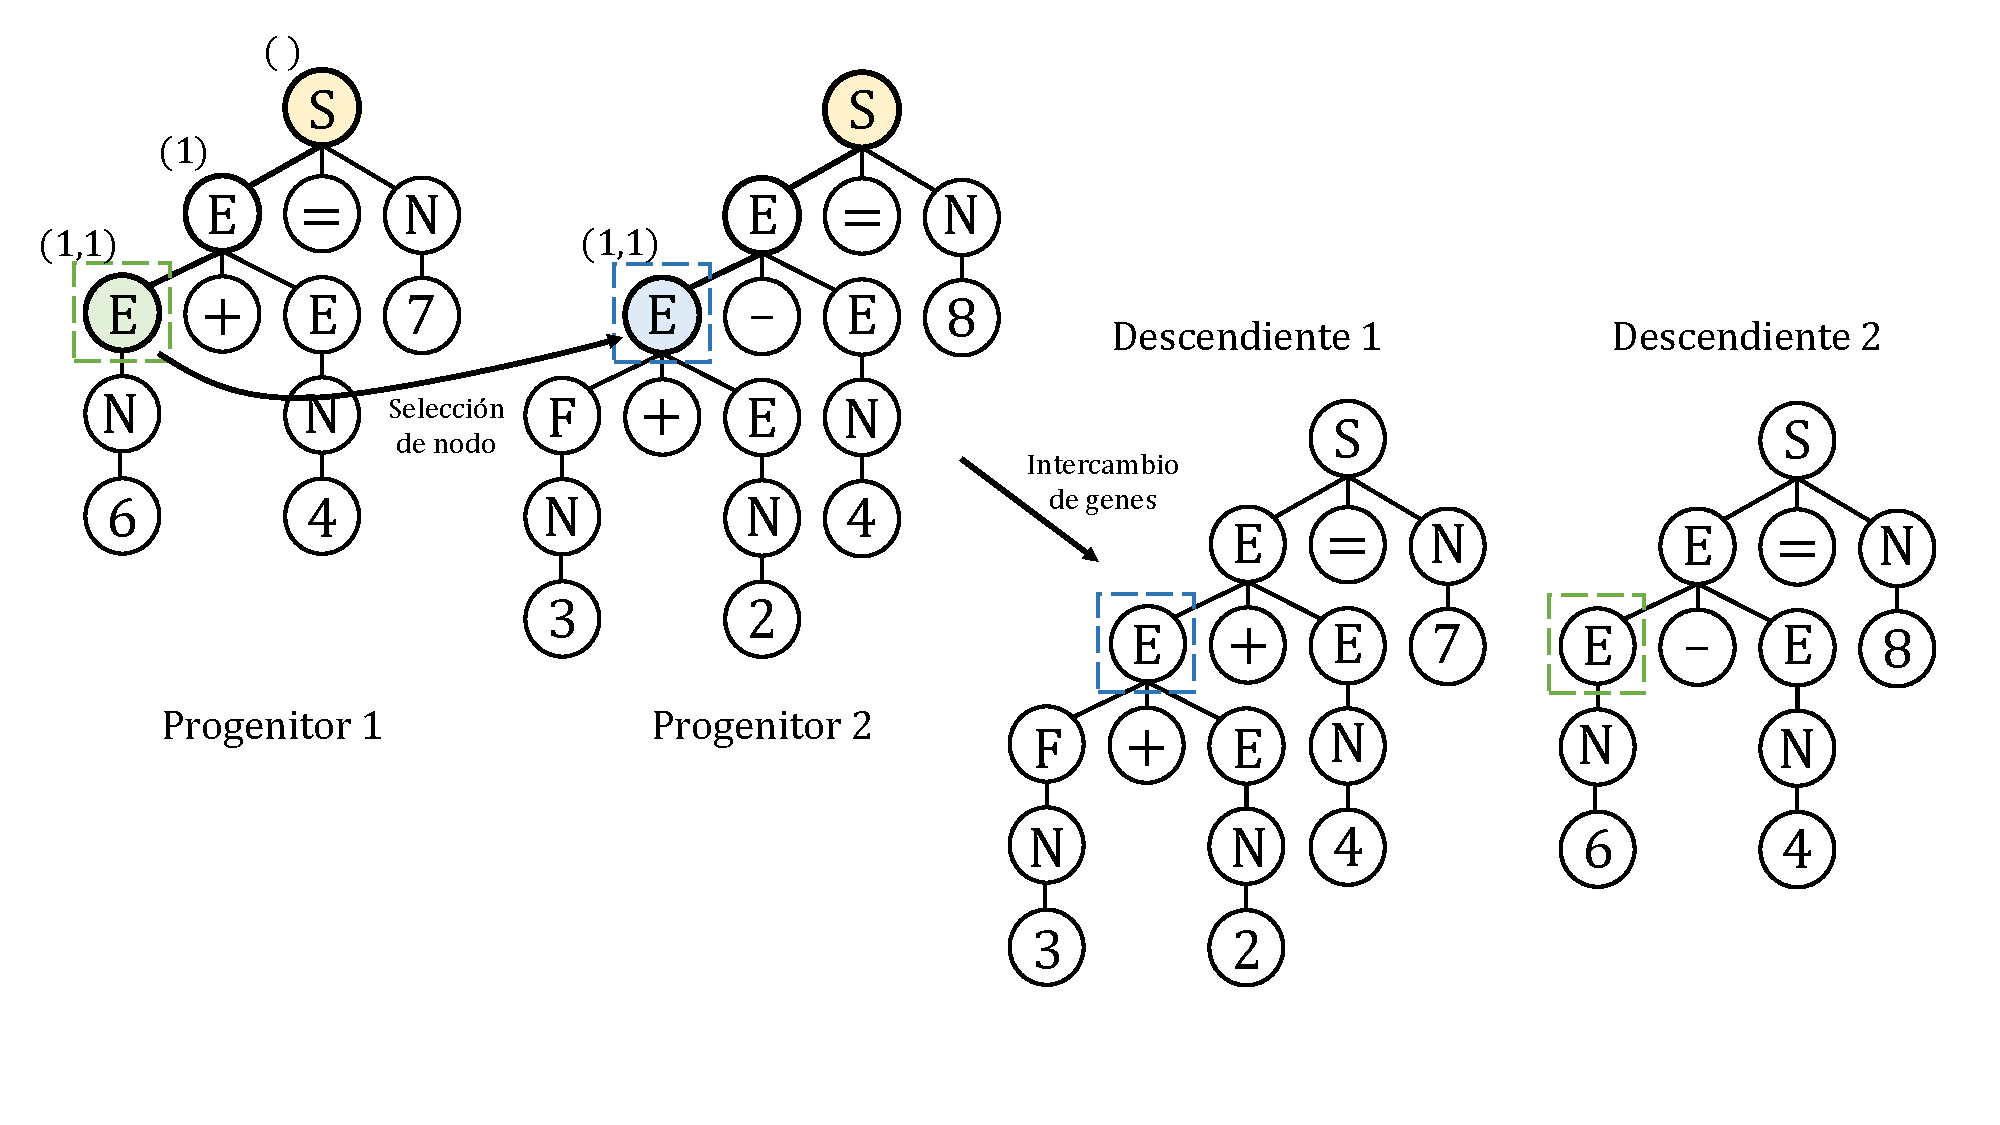
\includegraphics[width = 1\textwidth]{resources/Fig8.pdf}
          \caption{Ejemplo de aplicación del operador de cruce preservador del contexto.}
          \label{fig:8}
        \end{figure} \par \vfill
      
        \subsubsection*{\vspace{-0.5cm}{\normalsize Operador de cruce preservador del contexto}}
        \vspace{-0.5cm}
        El operador de cruce preservador del contexto (\emph{context preserving crossover}) (D'haeseleer, 1994) restringe el cruce sólo entre subárboles que tienen localizaciones similares. Estas localizaciones vienen dadas por las coordenadas, reduciendo el exceso de exploración del operador de Koza. Estas coordenadas se definen como el camino entre la raíz y el nodo elegido. Este cruce sólo selecciona un nodo aleatorio: el del primer progenitor. A continuación, extrae las coordenadas de ese nodo aleatorio y las busca en el segundo progenitor. Si esas coordenadas existen en el segundo progenitor, entonces cruza los árboles. En caso contrario, selecciona otro nodo aleatorio del primer padre, realizando ese proceso repetidamente hasta que se puede efectuar el cruce. En la Fig. \ref{fig:8} se puede observar el funcionamiento de este cruce. \par
        El problema que tiene es que es útil para individuos que son estructuralmente similares, es decir, que hay individuos que no se pueden cruzar, por lo que presenta serios problemas de exploración. Además, tiene amplia capacidad de explotación, por lo que, si bien es útil en fases tempranas del programa genético, puede producir una convergencia prematura y caídas en óptimos locales. Tampoco limita la profundidad de los árboles, por lo que propicia la aparición de intrones.
        
        \subsubsection*{\vspace{-0.5cm}{\normalsize Operador de Whigham}}
        \vspace{-0.5cm}
        El operador de Whigham (Whigham, 1995) busca establecer un equilibrio entre exploración y explotación. No utiliza las coordenadas, sino que selecciona un símbolo no terminal (exceptuando el axioma) del primer progenitor, y, a continuación, de los símbolos no terminales del segundo progenitor, selecciona uno aleatorio de entre aquellos que son iguales al nodo del primer progenitor. En la Fig. \ref{fig:9} se puede apreciar cómo funciona este operador. La única desventaja es que no controla la profundidad de los descendientes. \par
        \begin{figure}[H]
          \centering
          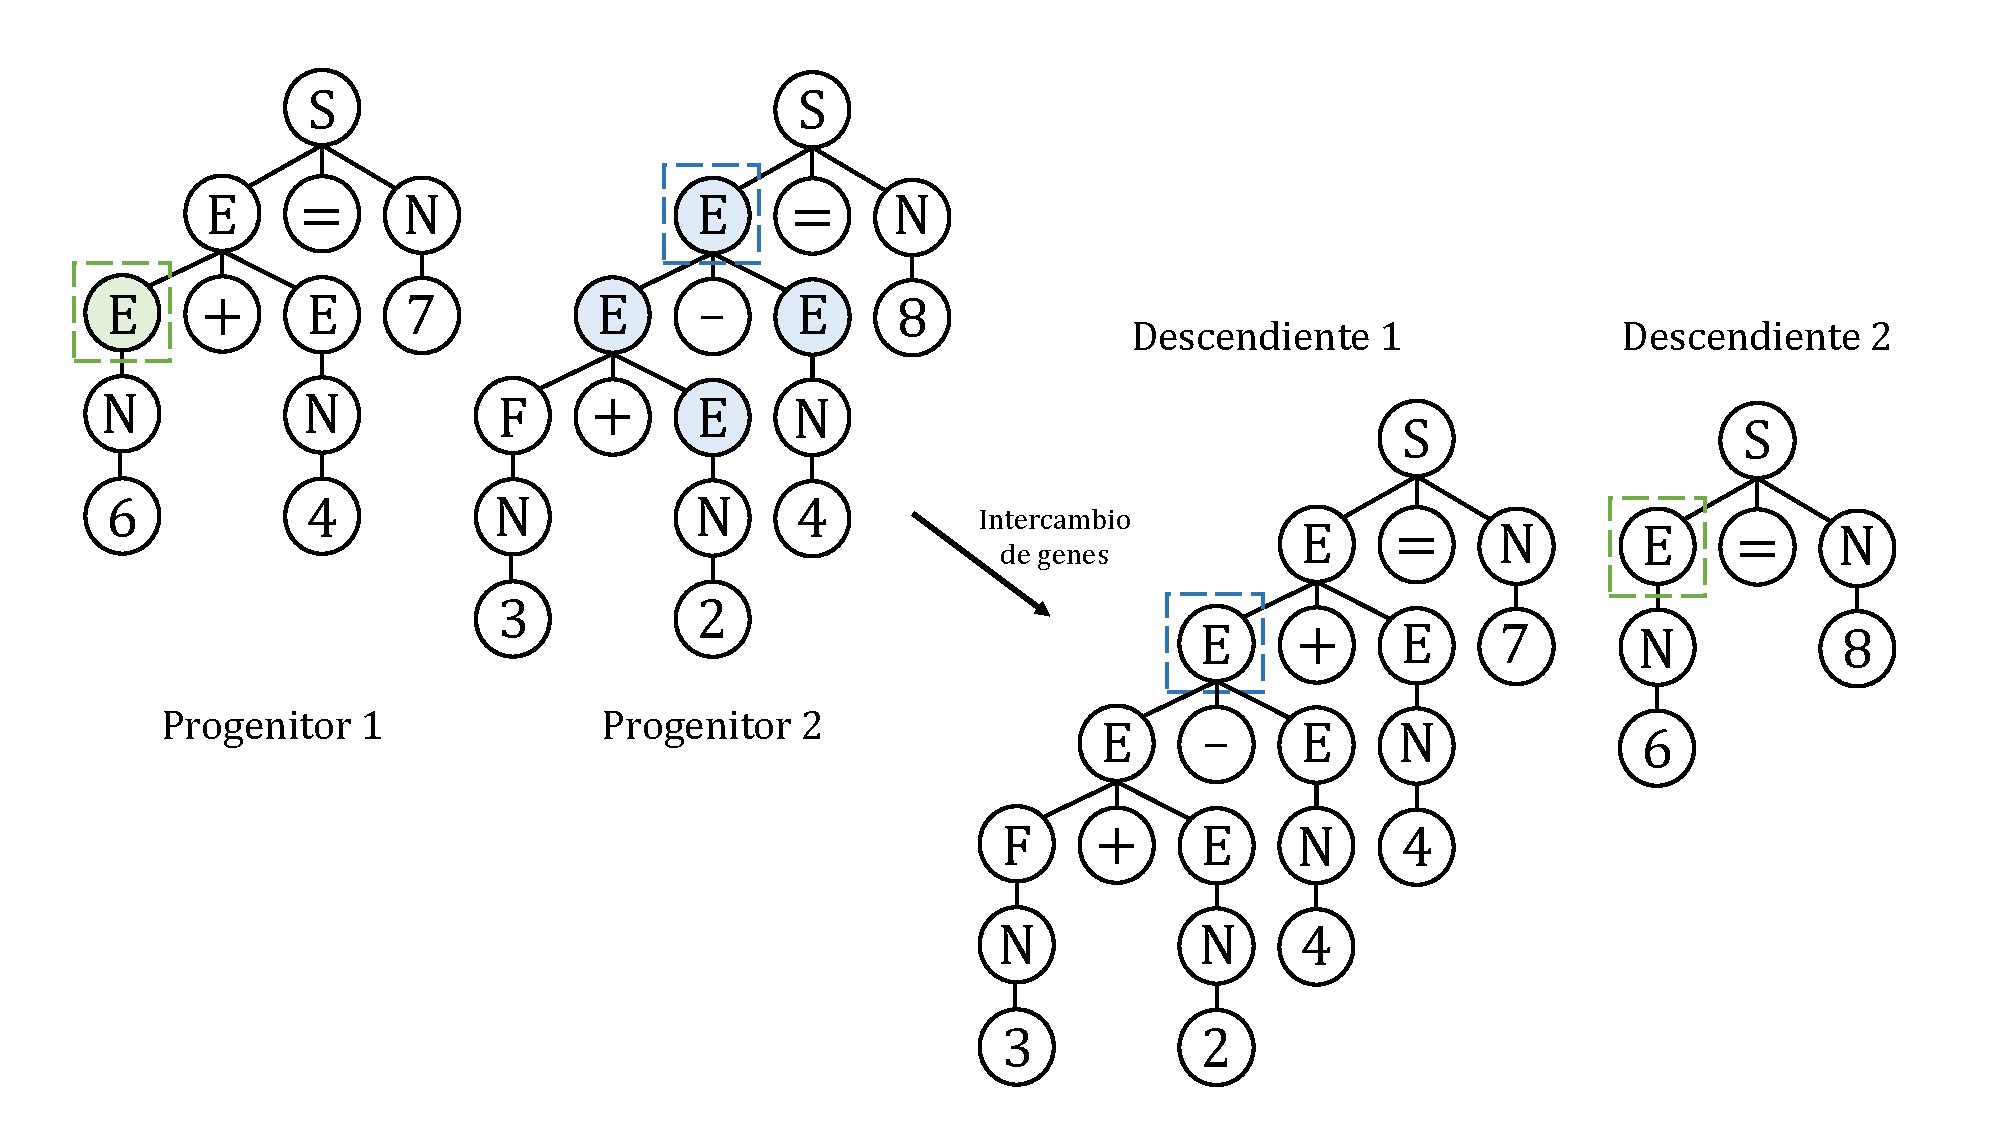
\includegraphics[width = 1\textwidth]{resources/Fig9.pdf}
          \caption{Ejemplo de aplicación del operador de cruce de Whigham.}
          \label{fig:9}
        \end{figure} \par
 
  \newpage\cleardoublepage
    
  \chapter{\vspace{-3cm}{\LARGE 3. Redes de Neuronas Artificiales}}
  \setcounter{figure}{9}
  \vspace{-1cm}
  Las Redes de Neuronas Artificiales son un modelo matemático inspirado en cómo el sistema nervioso procesa la información. El sistema nervioso está compuesto por un gran número de unidades de procesamiento de información denominadas neuronas (\emph{neurons}). En este capítulo se ofrece, en primer lugar, un resumen de la \emph{historia} de las Redes de Neuronas Artificiales. Seguidamente, un apartado de \emph{funcionamiento general} sobre esta rama de estudio y finalmente se describe la \emph{construcción de redes de neuronas} mediante la Programación Genética Guiada por Gramáticas. \par
  
    \section*{\Large 3.1. Historia}
    Los primeros trabajos sobre Redes de Neuronas Artificiales fueron las células de McCulloch y Pitts (McCulloch and Pitts, 1943) que no constituían redes ni tenían capacidad de aprendizaje. Pronto se verían reforzadas con las aportaciones de Hebb (Hebb, 1949) y Joseph Erlanger (1944). Sus descubrimientos sobre el aprendizaje humano y las fibras de conexión entre neuronas, respectivamente, fueron clave en los siguientes años de desarrollo de las Redes de Neuronas Artificiales. Pocos años después aparece el primer desarrollo metodológico basado en Redes de Neuronas Artificiales: el Perceptrón (\emph{perceptron}) (Rosenblatt, 1958, 1962), que incorpora un algoritmo de aprendizaje. \par
    Los años 60 destacó el trabajo de Widrow y Hoff (Widrow and Hoff, 1960): un sistema con un método de aprendizaje alternativo al Perceptrón llamado ADALINE (ADAptive LInear Element). Dos años después, estos científicos desarrollan una mejora adaptativa sobre su sistema (Widrow and Hoff, 1962). Esta década finaliza con la publicación del artículo \emph{Perceptrons} por Minsky y Papert (Minsky and Papert, 1969), en el que muestran las limitaciones de los perceptrones como el no poder resolver problemas no lineales como el problema del XOR. \par
    A raíz de esta última publicación, el interés sobre el estudio de estos modelos de aprendizaje se perdió, hasta tal punto que pasarían más de 10 años hasta la aparición de nuevos trabajos. Este silencio sería roto por Klopf (Klopf, 1972), quien formuló un mecanismo de aprendizaje adaptativo. También, apareció la primera publicación sobre una red multicapa para interpretar caracteres manuscritos: las Redes de Neuronas Artificiales Convolucionales (Fukushima, 1975). Este trabajo consigue despertar el interés de algunos investigadores, pero sin mucho éxito. \par
    Los años 80 y 90 fueron proganizados, en primer lugar, por la publicación del mapa (o red) de Kohonen (\emph{Kohonen map}) (Kohonen, 1982). En segundo lugar, se publicó un trabajo sobre de Redes de Neuronas Artificiales Recurrentes (Hopfield, 1982), que consiguió recobrar cierto interés en la investigación en este ámbito. La aparición, algunos años más tarde, del famoso método de aprendizaje de retropropagación del grediente (\emph{back-propagation learning method}) (Rumelhart et al., 1986) supone un hito en las redes neuronales que consigue el relanzamiento de esta disciplina.

% DEEP LEARNING
    
    \section*{\Large 3.2. Funcionamiento general}
    Las Redes de Neuronas Artificiales son un modelo de procesamiento inspirado en cómo los sistemas nerviosos en la biología procesan información. En términos simples, una Red de Neuronas Artificiales es un modelo matemático simplificado del cerebro que es utilizado para procesar relaciones no lineales entre las entradas y las salidas en paralelo tal y como hace el cerebro humano. \par
    En Fig. \ref{fig:10} se puede apreciar la arquitectura de un Perceptrón con una neurona artificial en la salida. Esta neurona recibe un conjunto determinado de entradas (en este caso, $n$), con sus respectivos pesos sinápticos $w_{i\thinspace j}$. A continuación, calcula el potencial sináptico como la suma de los productos entre las entradas por sus respectivos pesos. A este potencial se le aplica una función de activación, relativa a cada neurona, que permite devolver una salida $y$, en función del estado de activación. \par
    \begin{figure}[H]
      \centering
      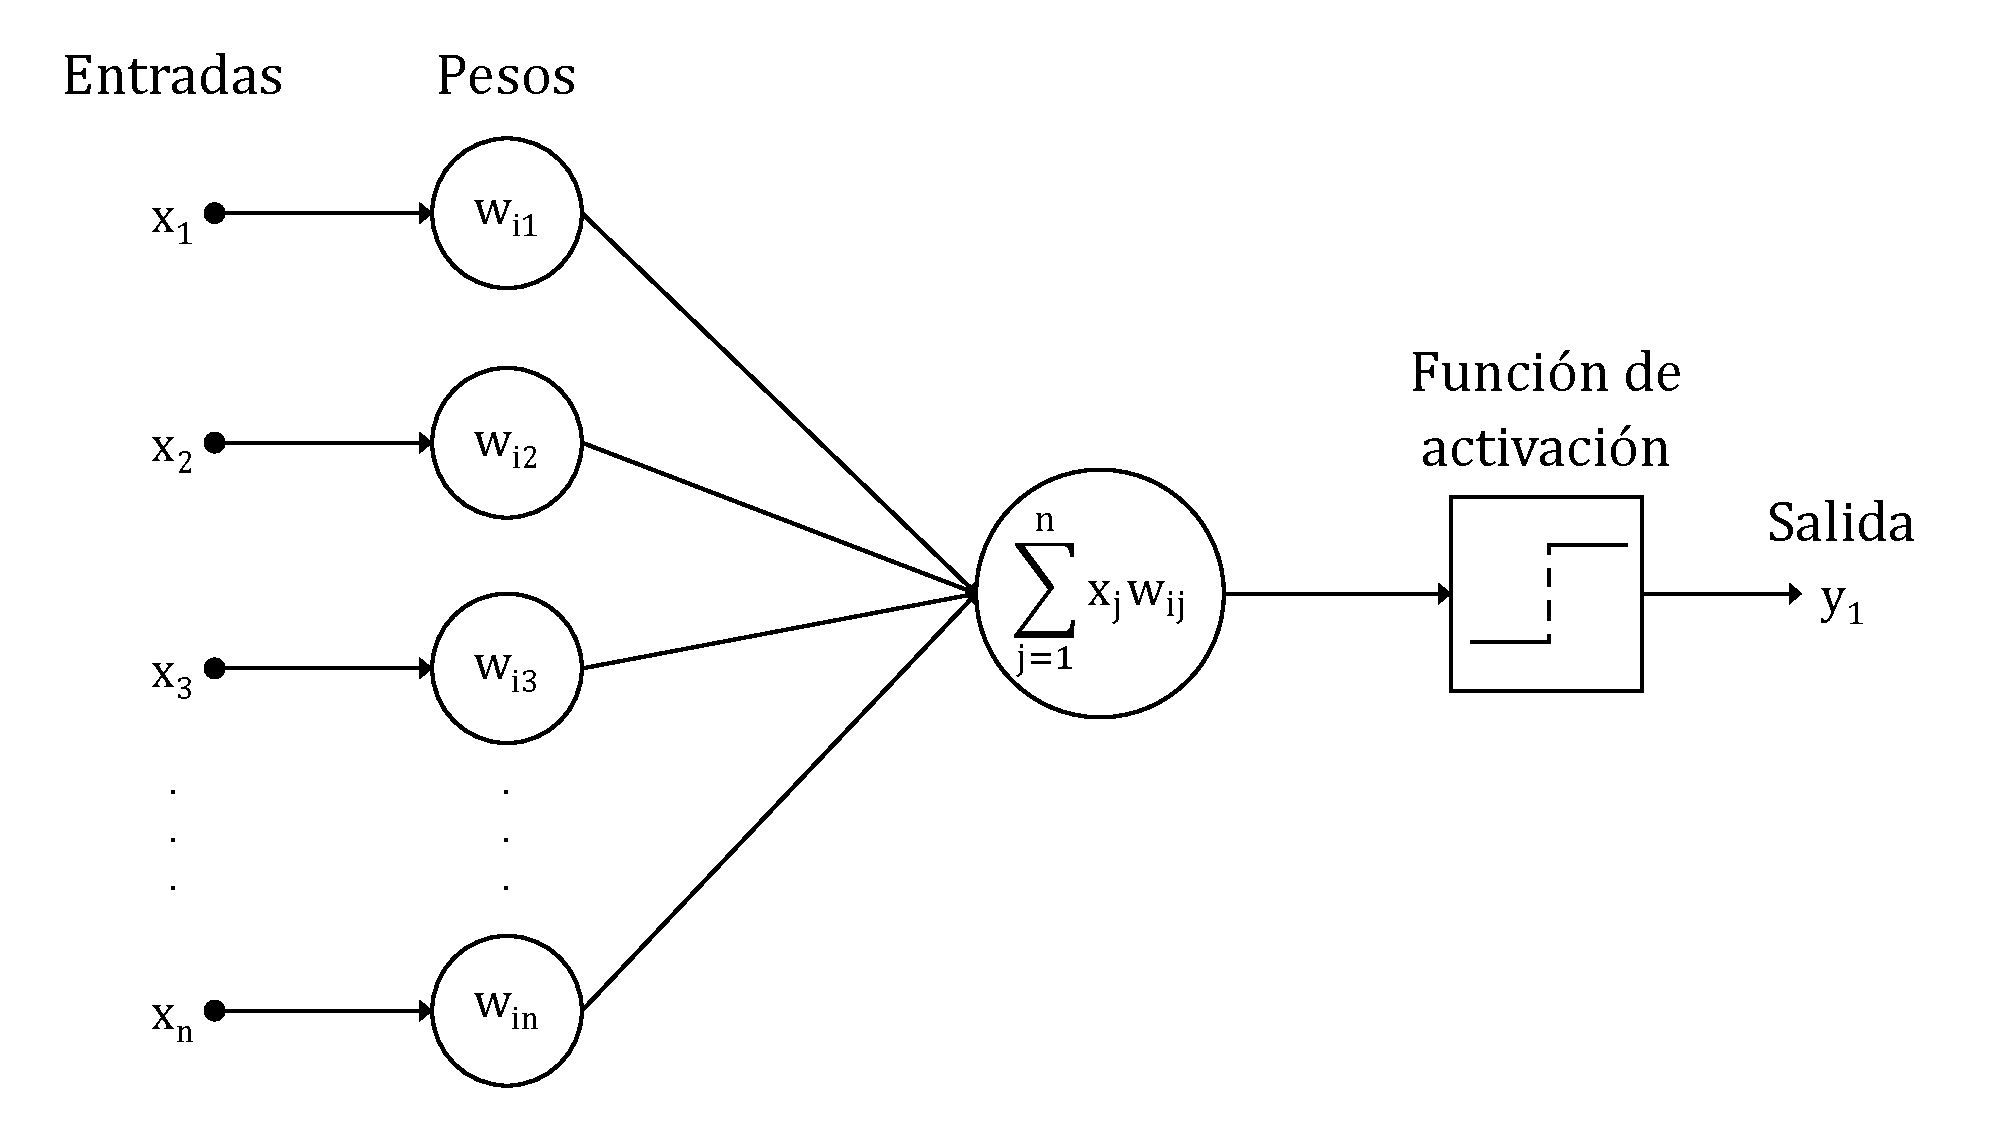
\includegraphics[width = 0.8\textwidth]{resources/Fig10.pdf}
      \caption{Arquitectura básica de un Perceptrón.}
      \label{fig:10}
    \end{figure} \par
    Actualmente, la arquitectura de una red general no es tan simple como la mostrada en la Fig. \ref{fig:10}. Una Red de Neuronas Artificiales suele componerse por, al menos, una capa oculta. Se establece, como regla general, que cuando una red tiene más de tres capas ocultas, se denomina Red de Neuronas Artificiales Profunda (Aizenberg et al., 2000). En Fig. 11 se muestra una arquitectura neuronal 2 capas ocultas. Además, esta red es alimentada hacia delante; modelo utilizado en este trabajo. \par
    \begin{figure}[H]
      \centering
      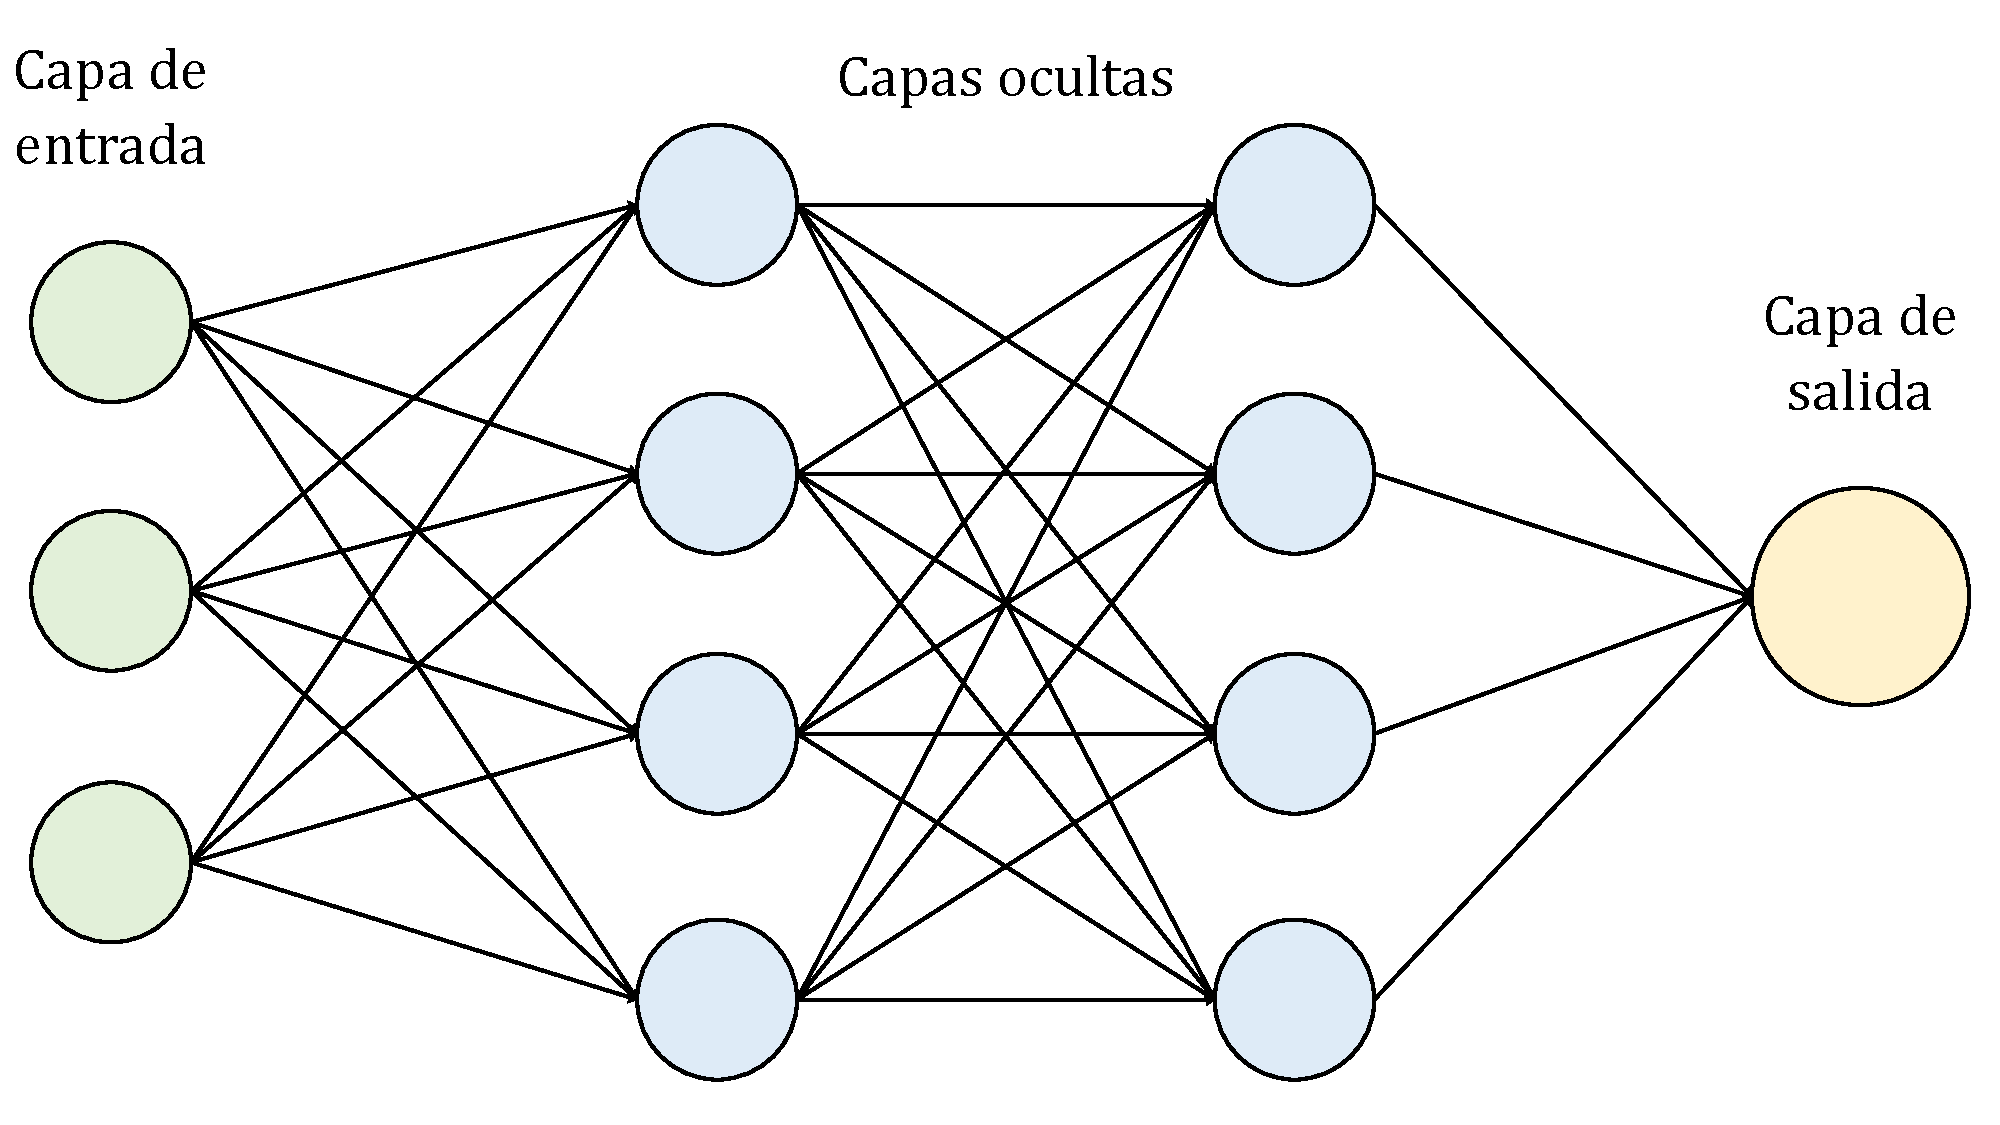
\includegraphics[width = 0.8\textwidth]{resources/Fig11.pdf}
      \caption{Distintas capas de una Red de Neuronas Artificiales.}
      \label{fig:11}
    \end{figure} \par
    En la capa de entrada, las neuronas reciben datos o señales procedentes del entorno. Las neuronas de la capa de salida proporcionan la respuesta del modelo a los estímulos de la entrada, aplicando una transformación que se lleva a cabo en la red. Entre la capa de entrada y la de salida están las capas ocultas (\emph{hidden layers}), que no reciben ni suministran informacion al entorno, sino que la modifican ya que llevan a cabo el procesamiento interno de la red. \par
    El proceso que sigue una Red de Neuronas Artificiales al actualizar los pesos se denomina aprendizaje. En el aprendizaje supervisado, modelo utilizado en este trabajo, la red conoce la salida correcta ante cada entrada, por lo que el objetivo es minimizar el error entre el valor que predice la red y su valor deseado. En cambio, en el aprendizaje no supervisado, la red recibe un conjunto de patrones de los que no conoce la respuesta deseada. En este caso, extrae patrones y relaciones entre los datos. \par
    Cada neurona oculta o de salida tiene asociada una función de activación. En la Fig. \ref{fig:12} se muestran las funciones de activación más destacadas.
    \begin{figure}[H]
      \begin{minipage}{0.49\textwidth}
        \centering
        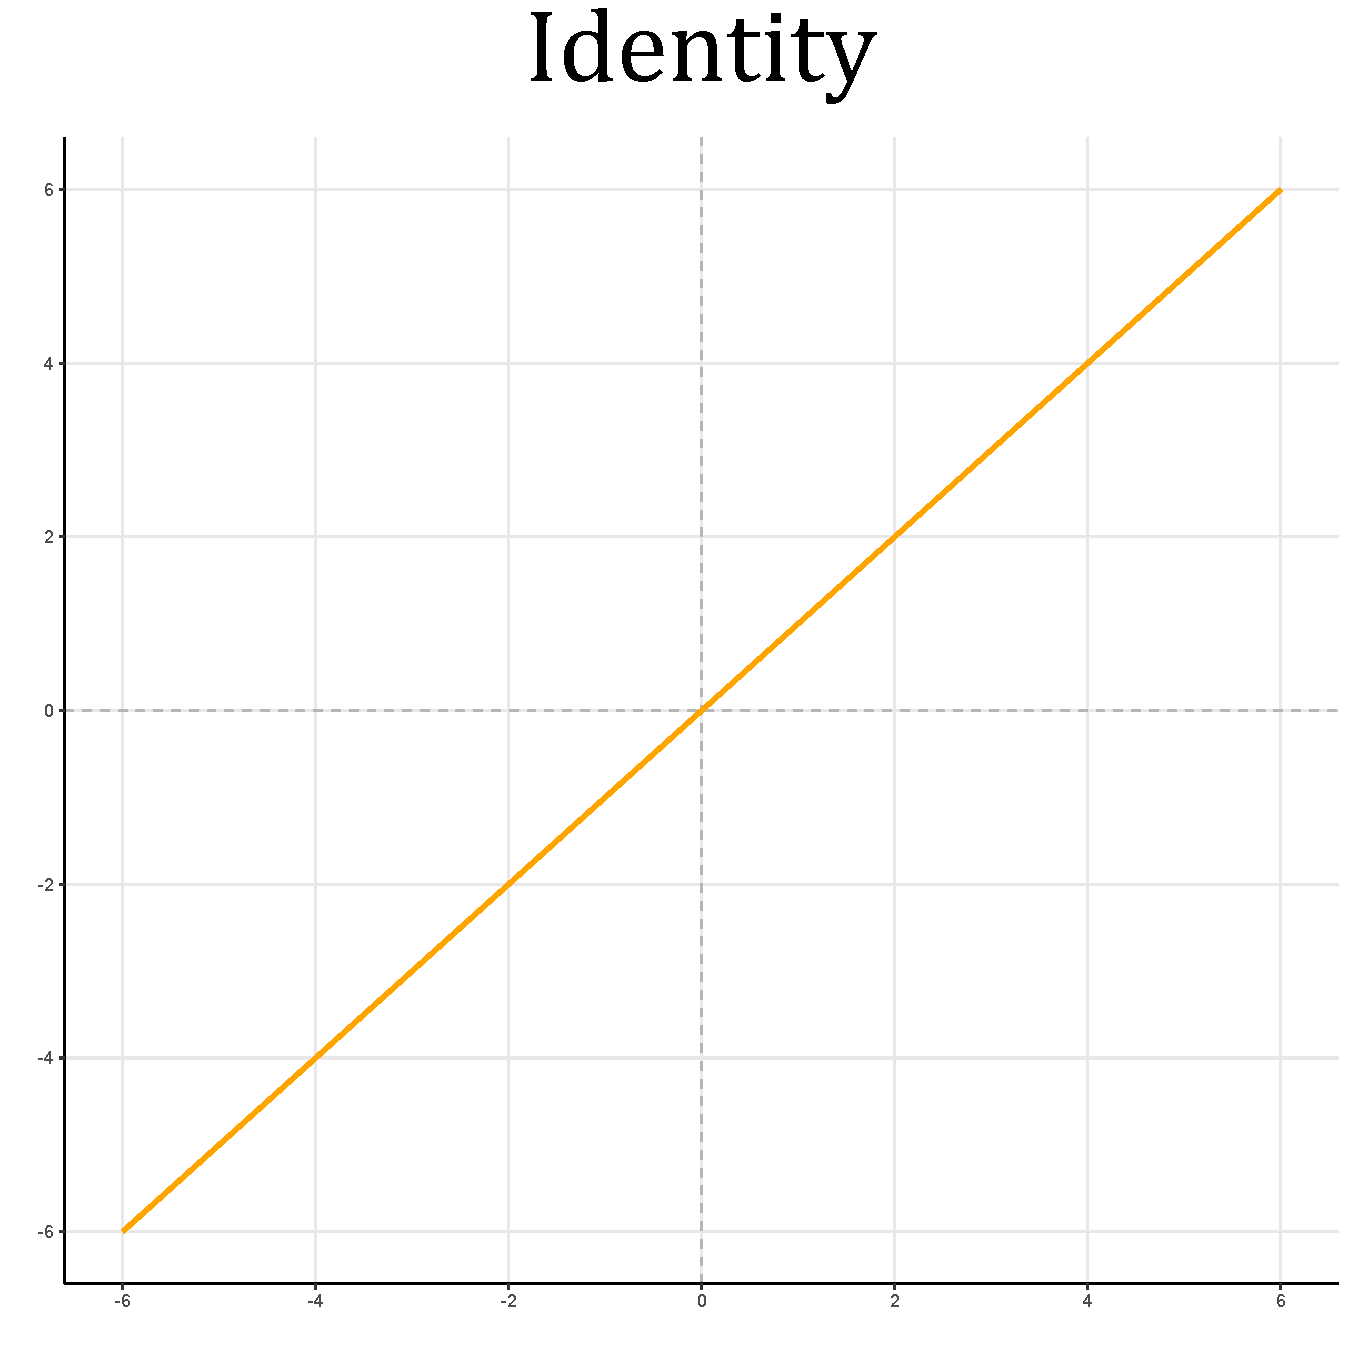
\includegraphics[width = 1\linewidth]{resources/Fig12_1.pdf}
      \end{minipage}
      \begin{minipage}{0.49\textwidth}
        \centering
        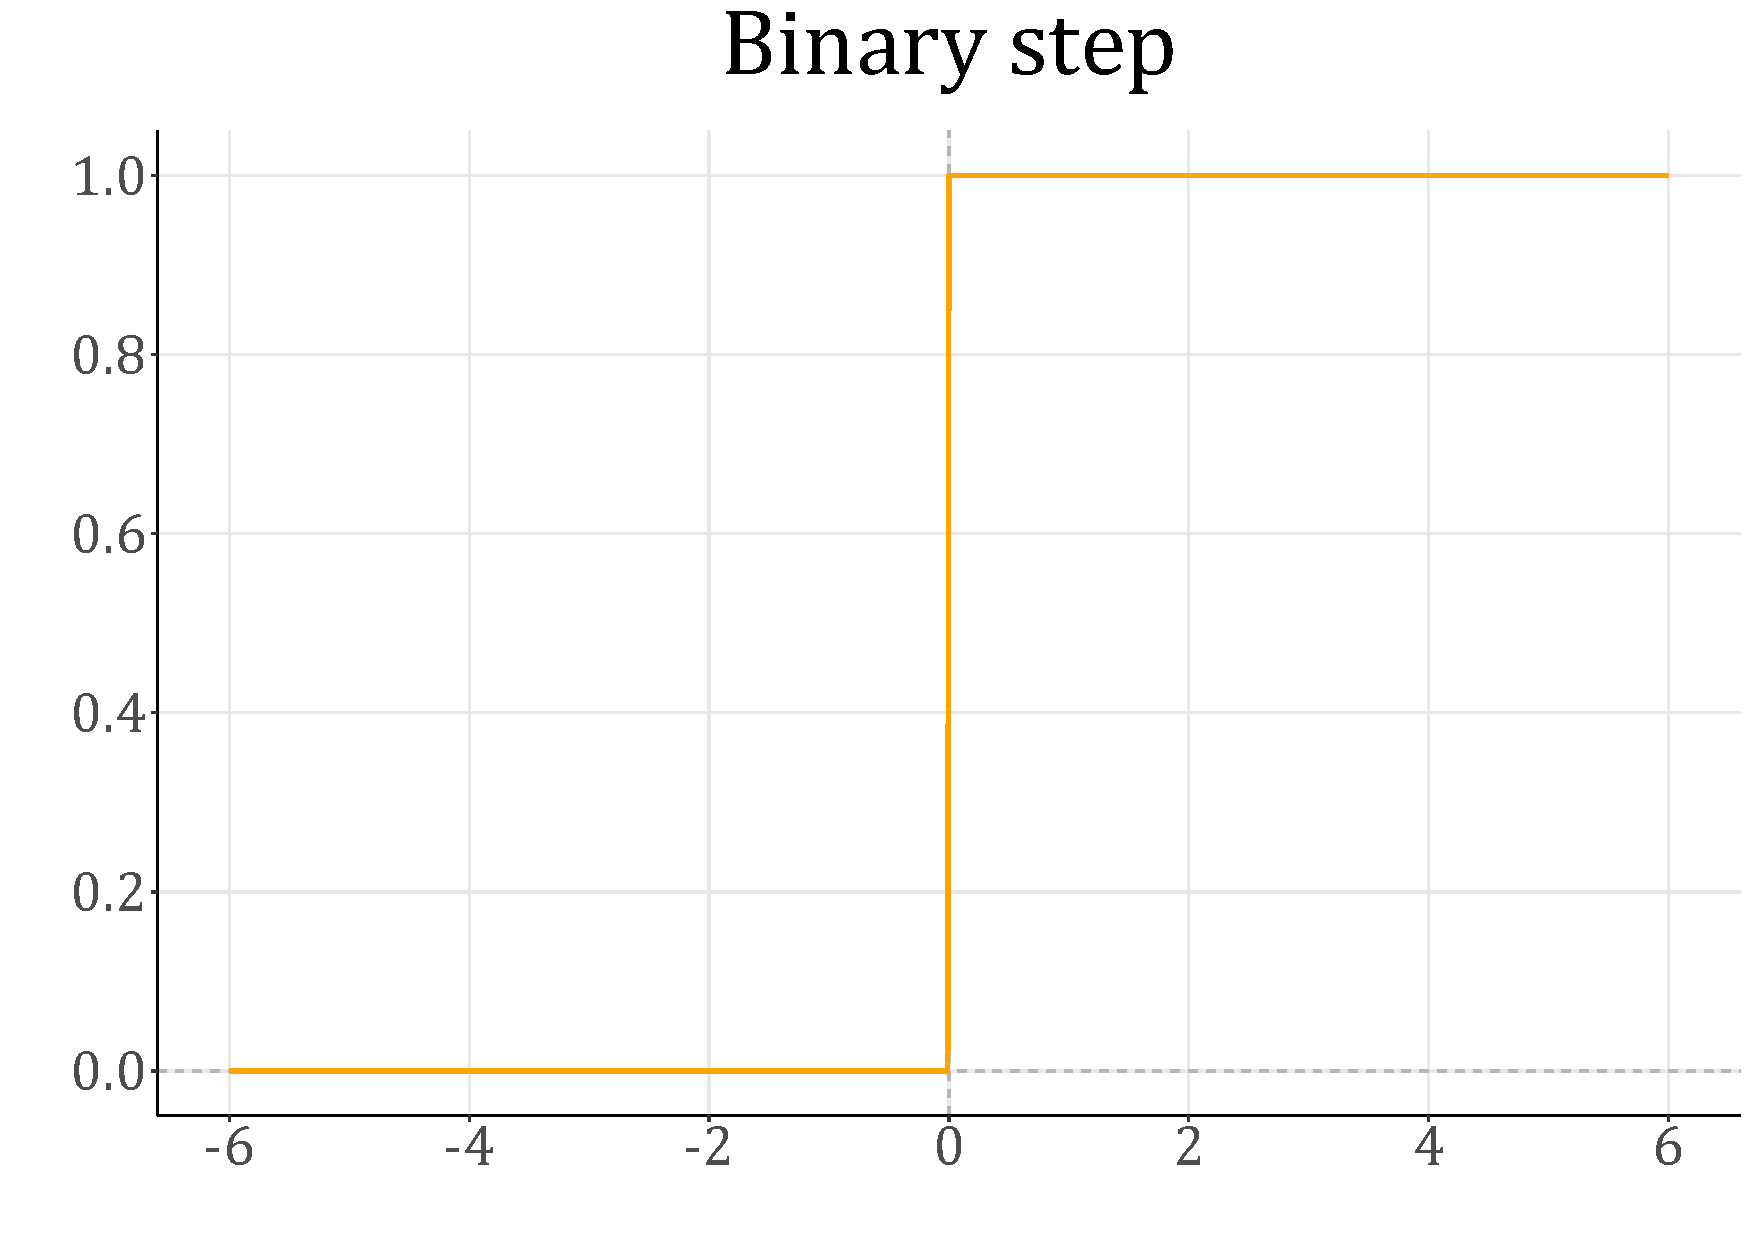
\includegraphics[width = 1\linewidth]{resources/Fig12_2.pdf}
      \end{minipage}
    \end{figure} \vfill
    \begin{figure}[H]
      \begin{minipage}{0.49\textwidth}
        \centering
        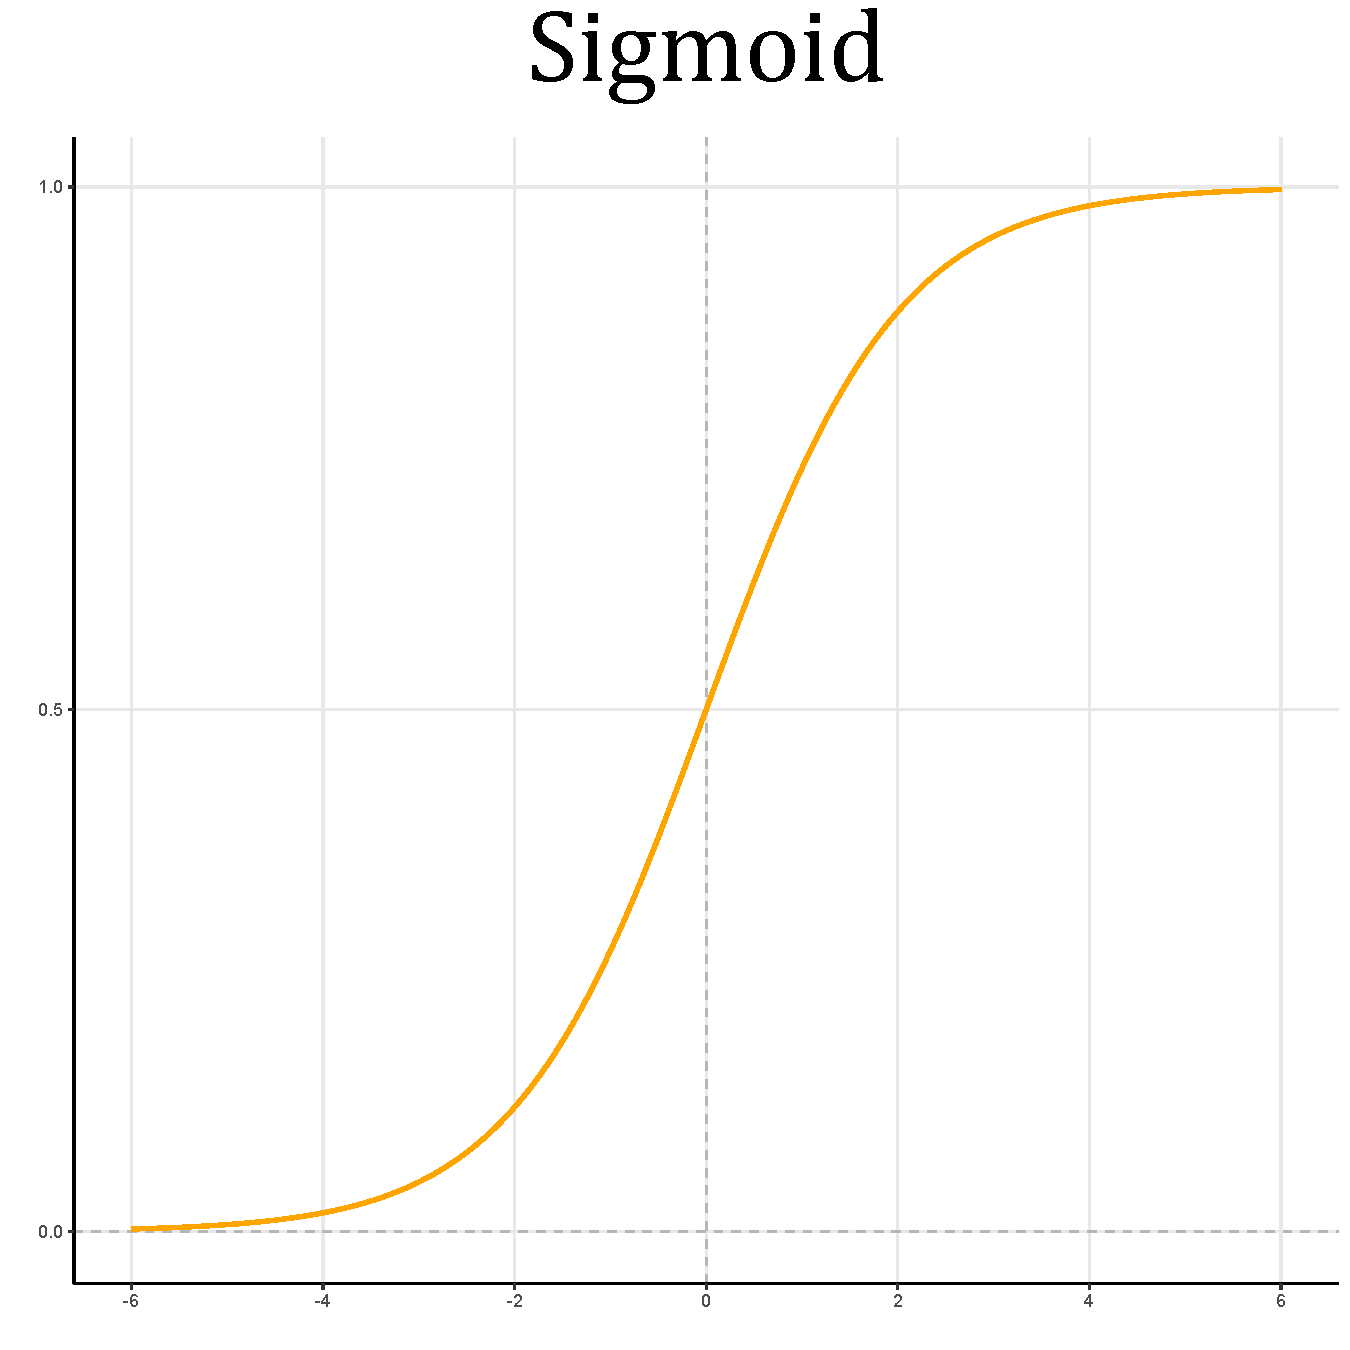
\includegraphics[width = 1\linewidth]{resources/Fig12_3.pdf}
      \end{minipage}
      \begin{minipage}{0.49\textwidth}
        \centering
        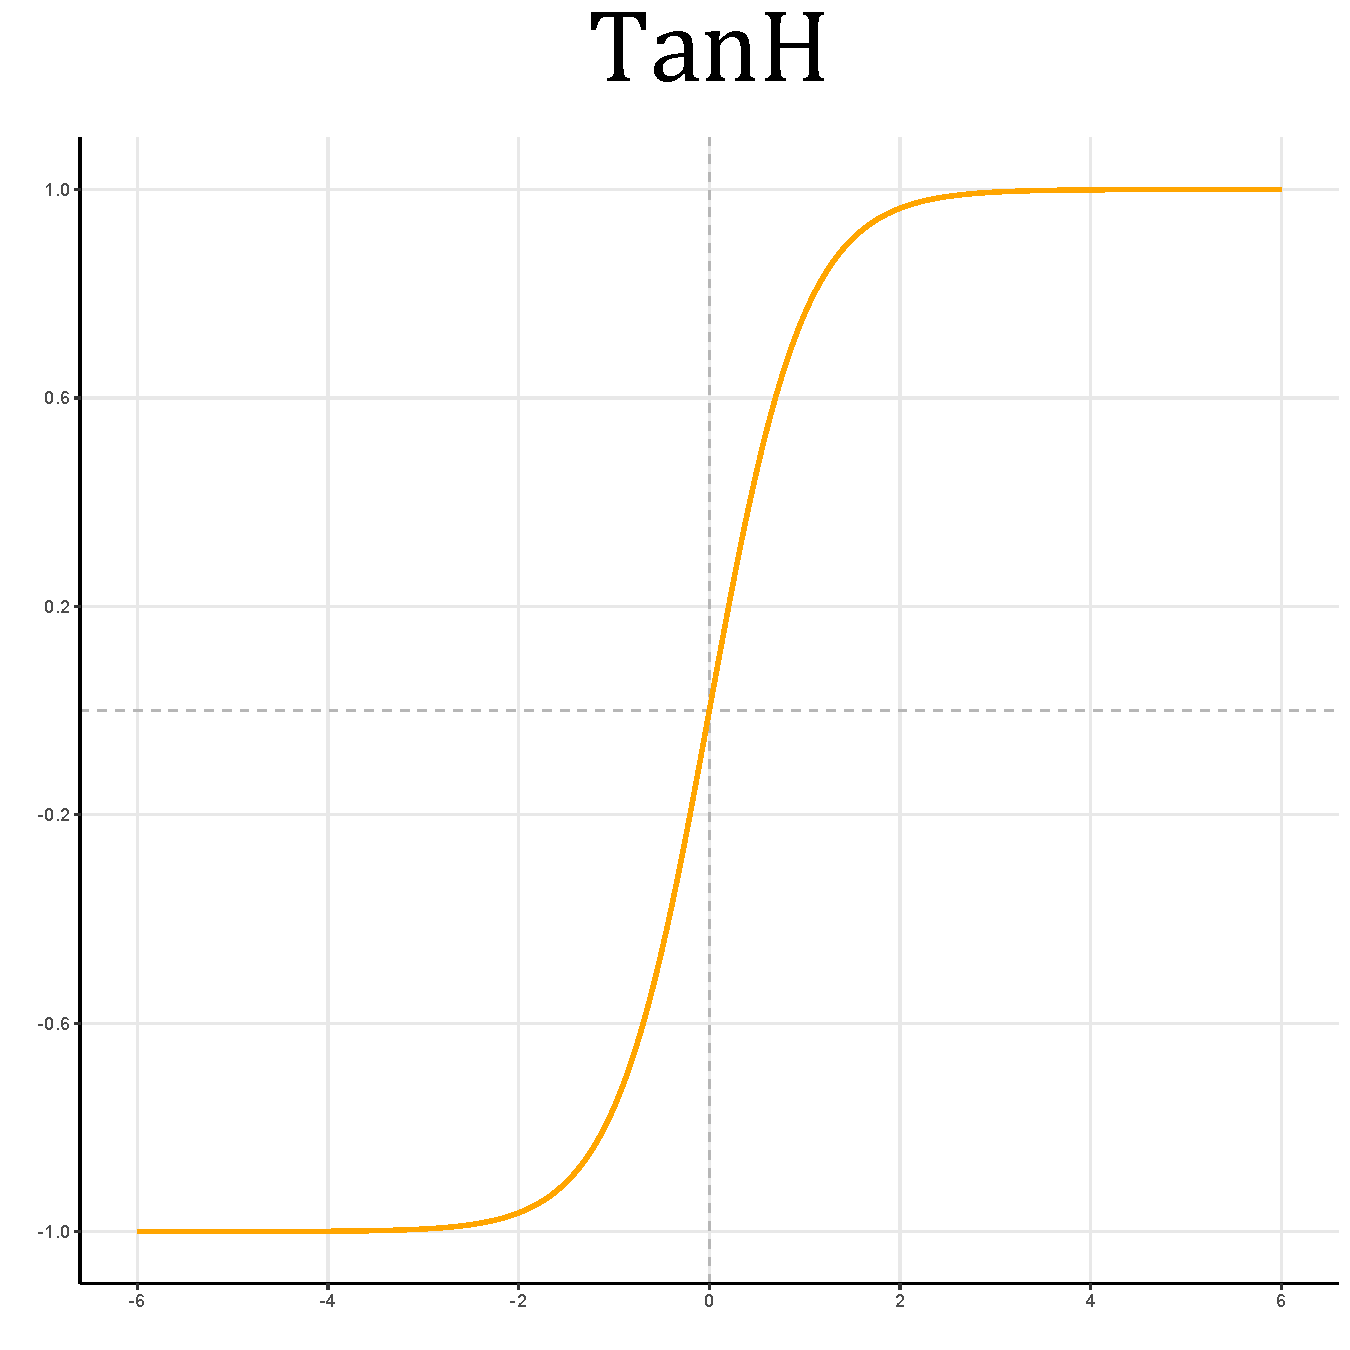
\includegraphics[width = 1\linewidth]{resources/Fig12_4.pdf}
      \end{minipage}
    \end{figure}
    \begin{figure}[H]
      \begin{minipage}{0.49\textwidth}
        \centering
        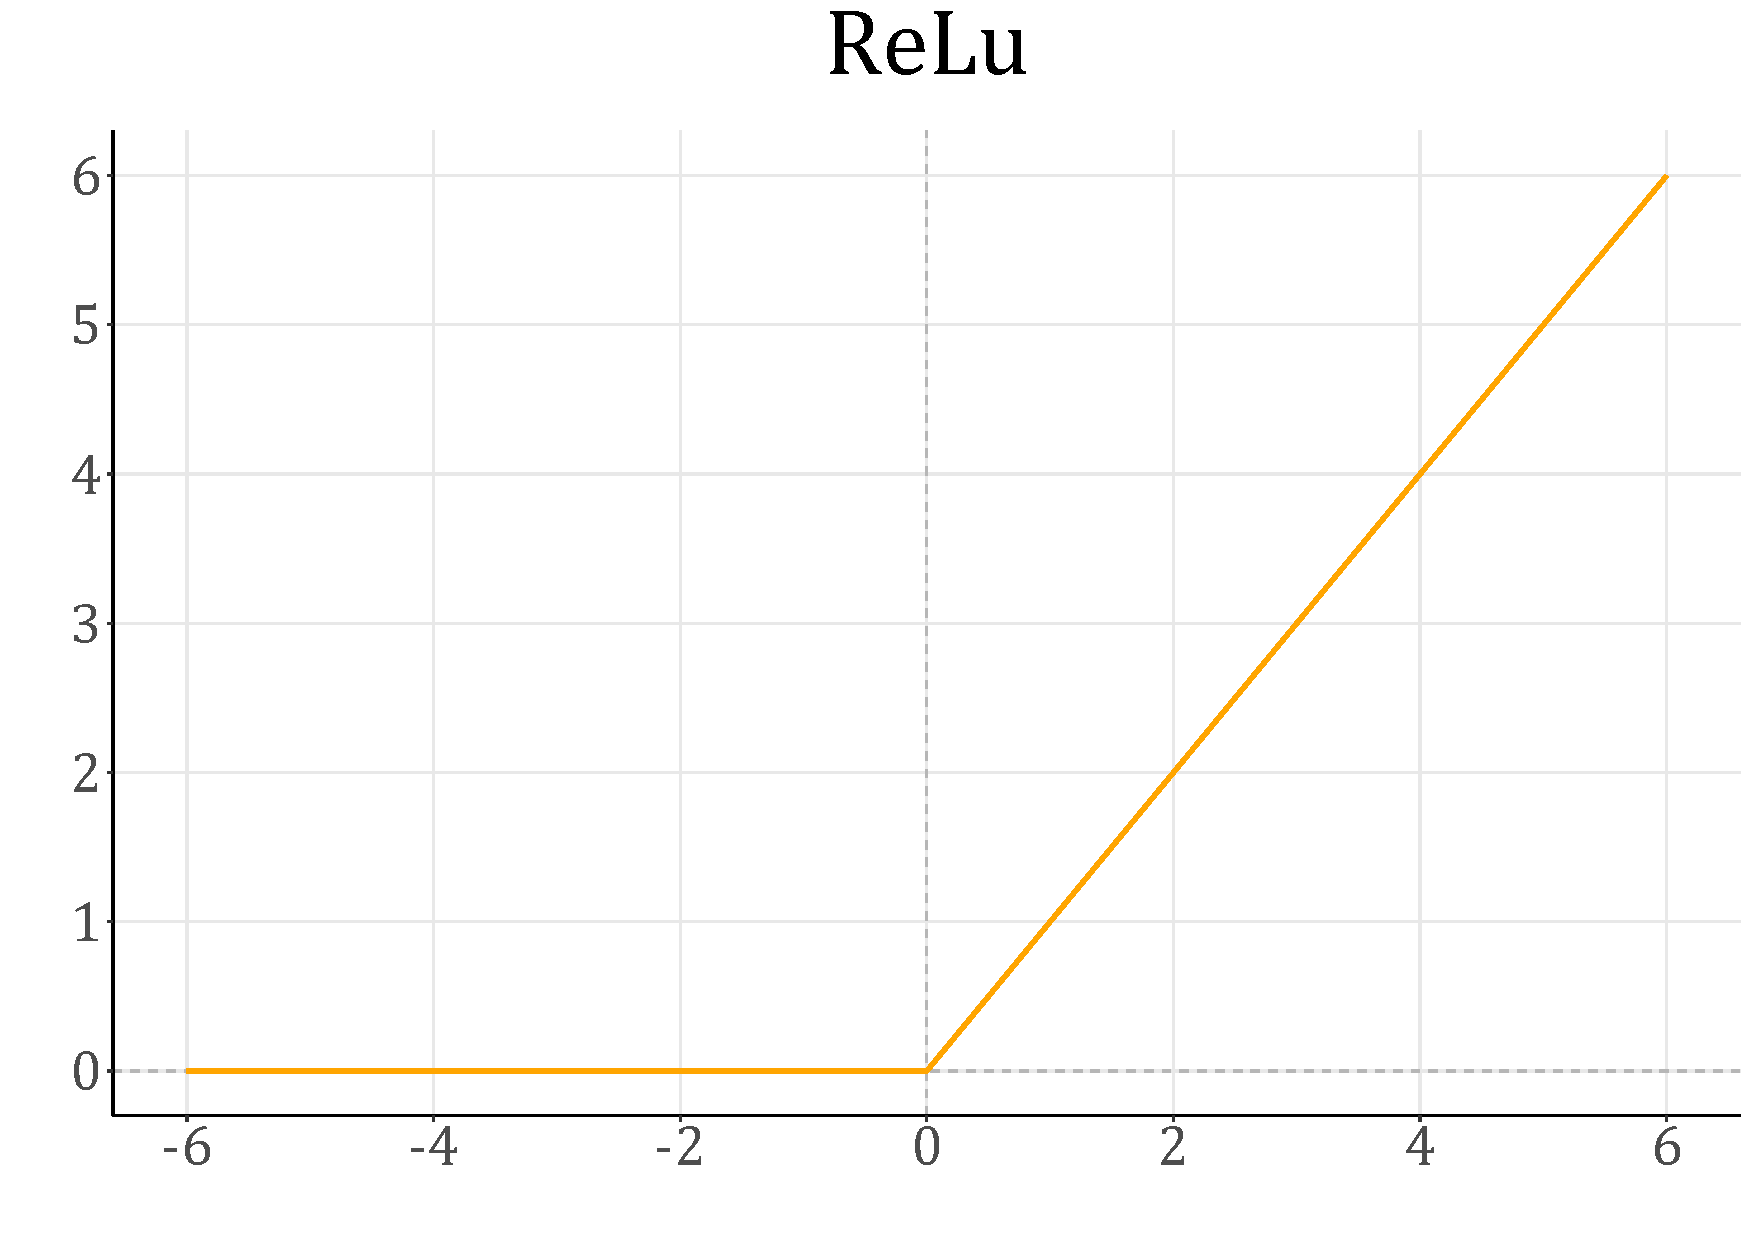
\includegraphics[width = 1\linewidth]{resources/Fig12_5.pdf}
      \end{minipage}
      \begin{minipage}{0.49\textwidth}
        \centering
        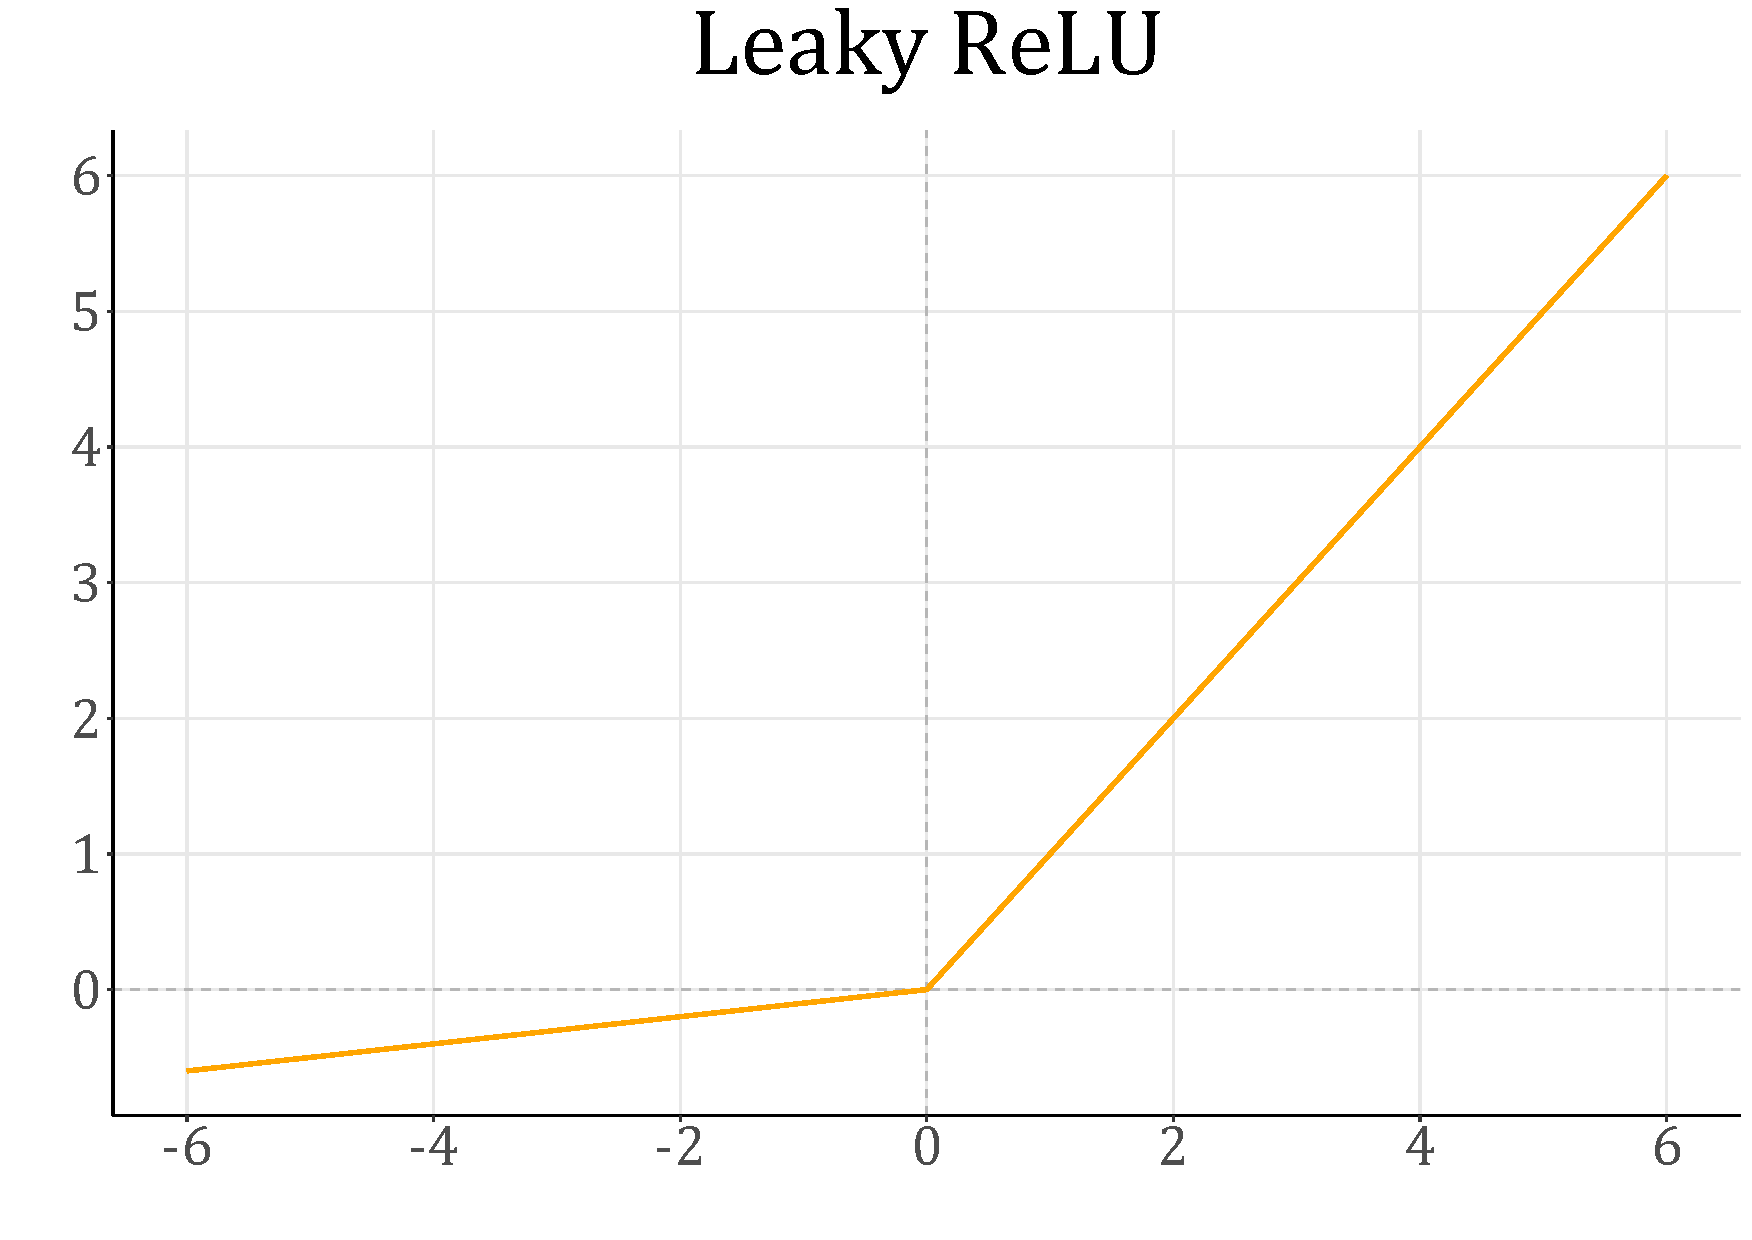
\includegraphics[width = 1\linewidth]{resources/Fig12_6.pdf}
      \end{minipage}
    \end{figure}
    \begin{figure}[H]
      \begin{minipage}{0.49\textwidth}
        \centering
        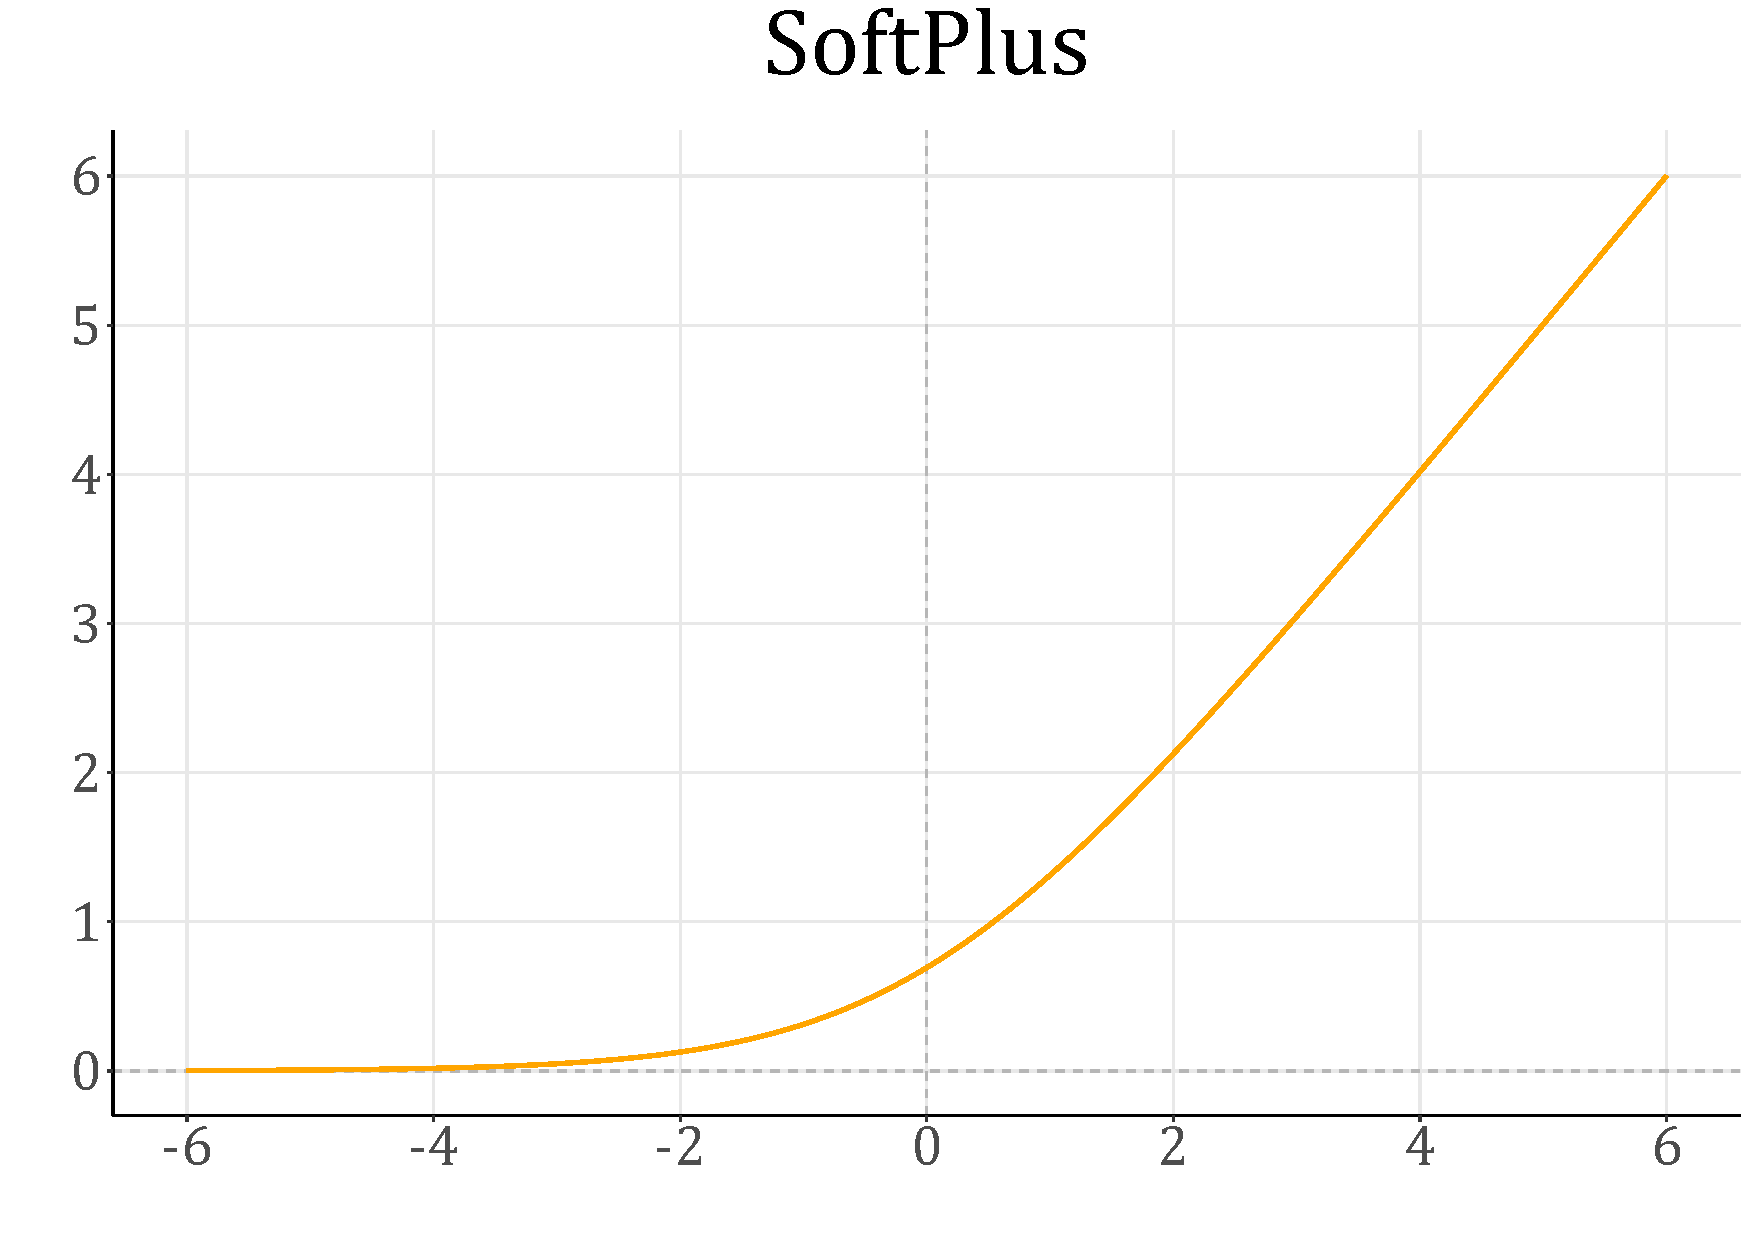
\includegraphics[width = 1\linewidth]{resources/Fig12_7.pdf}
      \end{minipage}
      \begin{minipage}{0.49\textwidth}
        \centering
        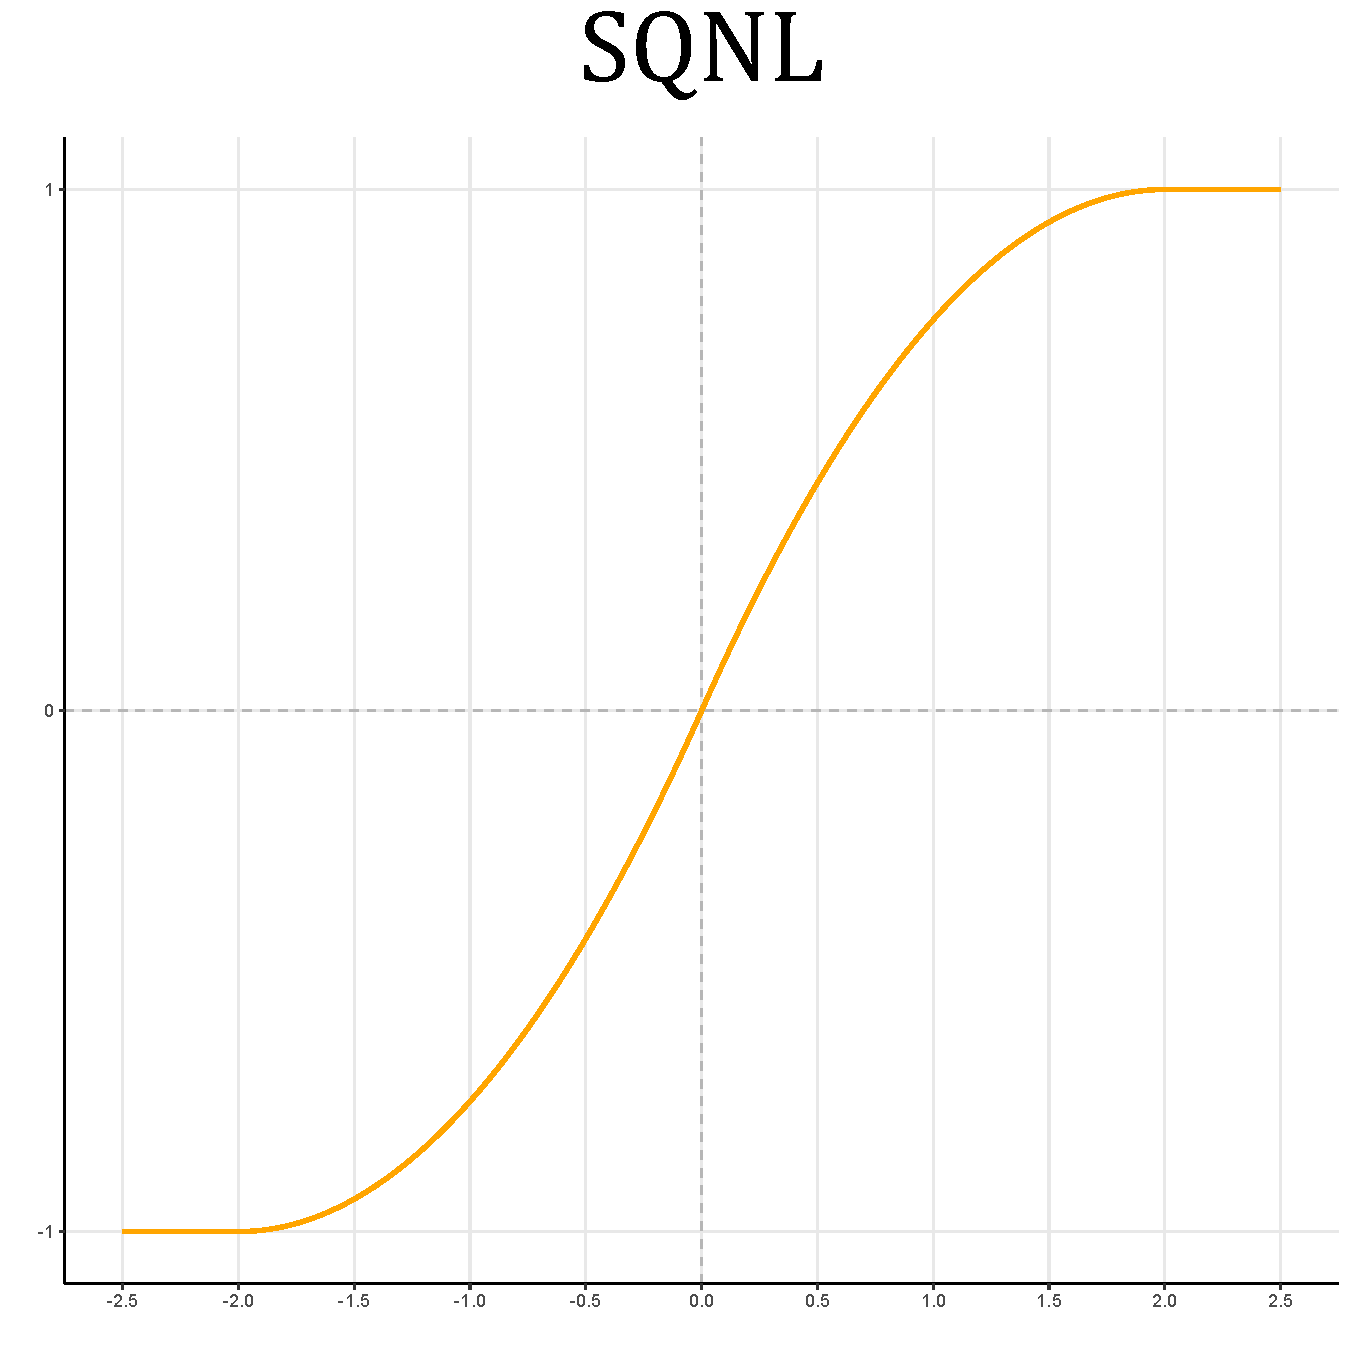
\includegraphics[width = 1\linewidth]{resources/Fig12_8.pdf}
      \end{minipage}
      \caption{Gráficas de las funciones de activación más utilizadas.}
      \label{fig:12}
    \end{figure} \par
    El proceso de entrenamiento supervisado de una red comienza tras asignar unos valores iniciales a los pesos de la red de forma aleatoria. Tras asignar estos pesos iniciales, procesa las entradas y compara las salidas predichas con las esperadas. Si hay errores en la predicción, entonces los gredientes del error se propagan hacia atrás en la red, provocando la actualización de los pesos de sus conexiones, a fin de minimizar el error entre el valor de la salida predicha por la red y el valor de la salida esperado. \par
    La red utiliza el conjunto de entrenamiento durante todo el proceso, que tiene una duración limitada, medida en épocas (\emph{epochs}), que es el número de veces que la red utiliza los datos provistos para entrenar y ajustar los pesos de sus conexiones.
    
    \section*{\Large 3.3. Deep Learning}
    El Aprendizaje Profundo (\emph{deep learning}) es un subcampo del Aprendizaje Automático y basado en Redes de Neuronas Artificiales. Se considera que una red es profunda si tiene más de tres capas ocultas. \par
    Una de las aplicaciones más destacadas del Deep Learning es lo relativo a clasificación de imágenes con Redes de Neuronas Convolucionales (Fukushima, 1975). La diferencia más notable entre este tipo de aprendizaje y el Aprendizaje Automático reside en que en el segundo tipo es necesario un proceso de extracción manual de las características relevantes de las imágenes, a partir de las cuales se entrena un modelo que aprende de ellas. En el Deep Learning, las características las aprende el modelo, provisto de datos (imágenes) sin procesar. \par
    \begin{figure}[H]
      \centering
      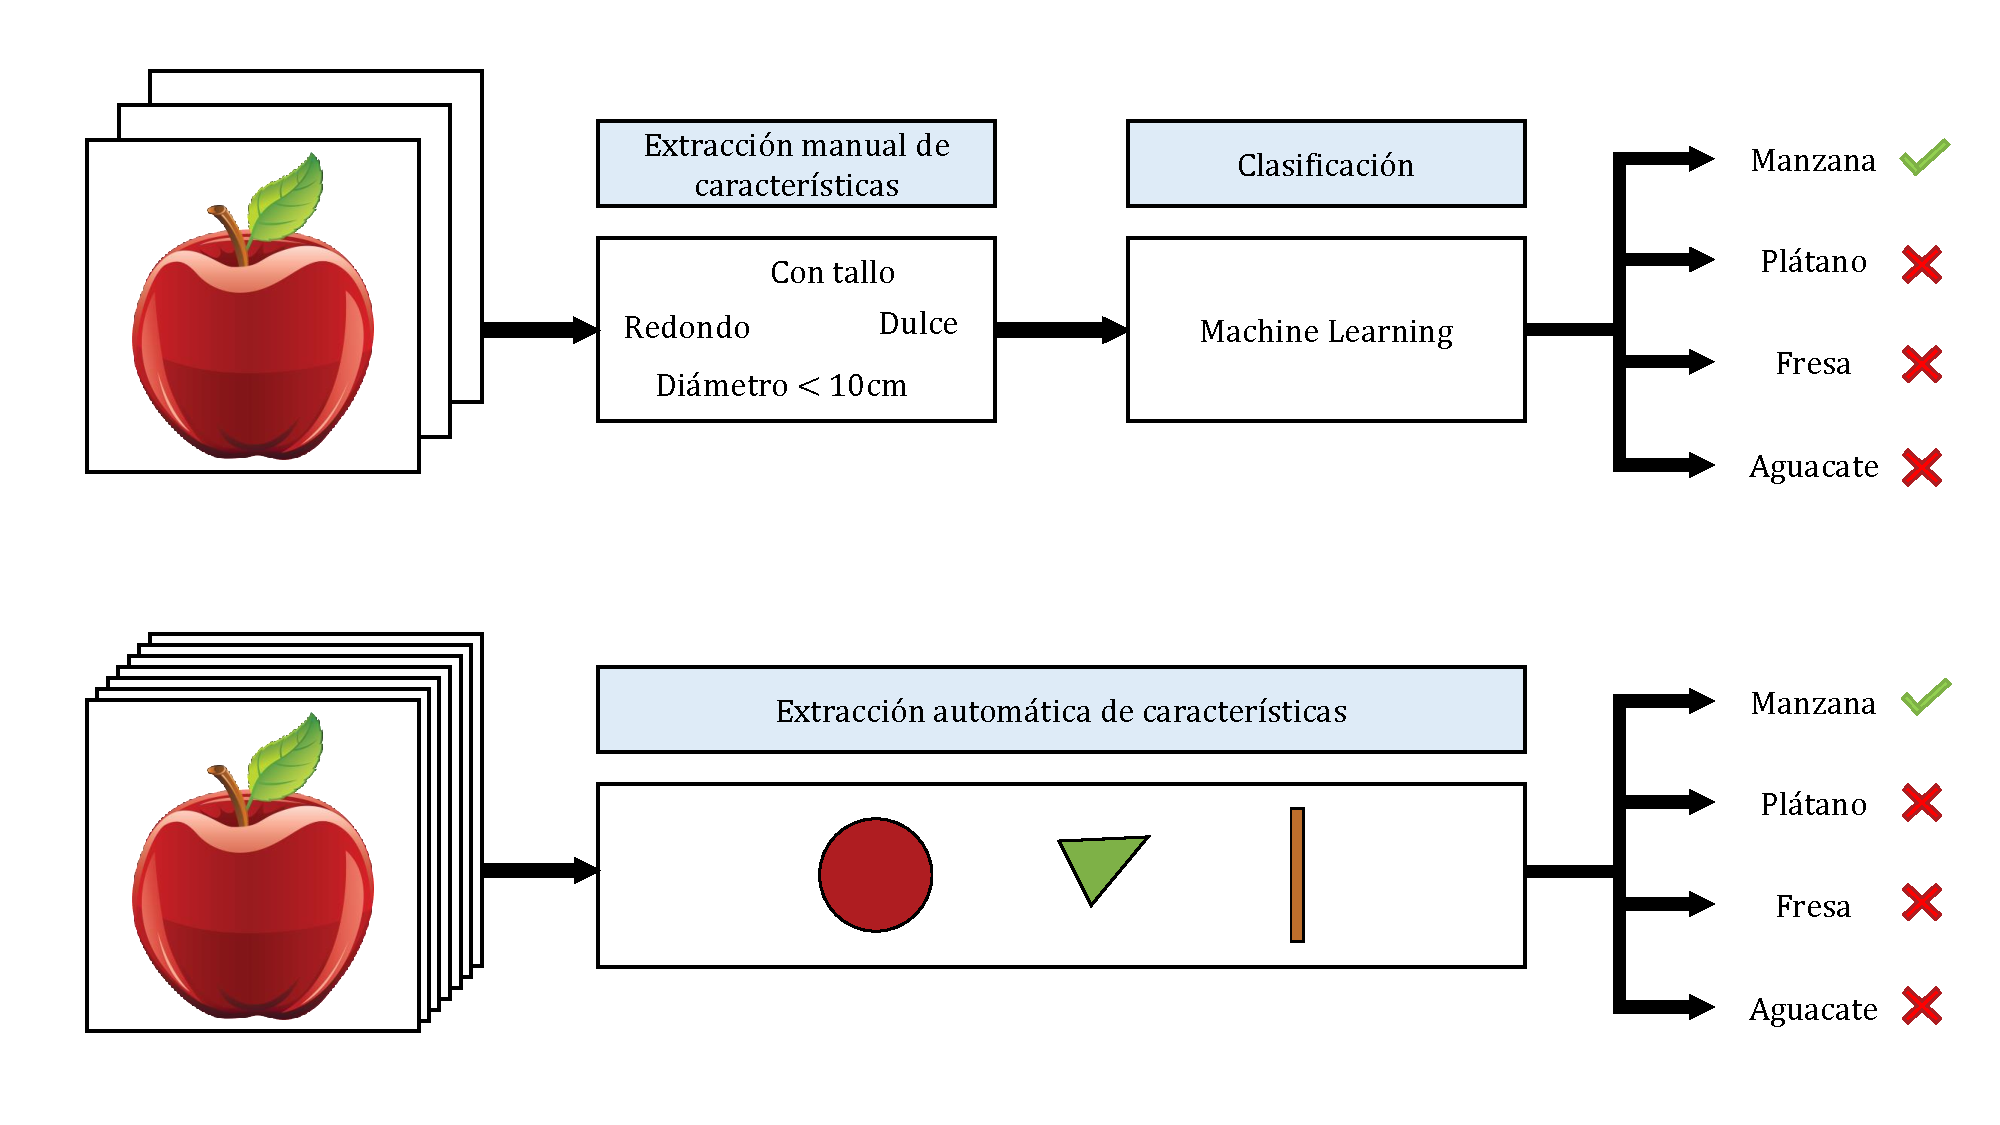
\includegraphics[width = 1\textwidth]{resources/Fig13.pdf}
      \caption{Ejemplo de Red de Neuronas Artificiales Profunda.}
      \label{fig:13}
    \end{figure}
    En la Fig. \ref{fig:13}, se muestra una comparativa entre el Aprendizaje Automático y el Deep Learning. En ambos se utilizan Redes de Neuronas Artificiales. En el diagrama superior, se detalla el funcionamiento del Aprendizaje Automático, en el que se utiliza poca cantidad de datos, de los que se extraen características manualmente. Estas características son utilizadas para realizar predecciones. En el diagrama inferior, se detalla el funcionamiento del Deep Learning, en el que, en contraposición del Aprendizaje Automático, se utiliza una gran cantidad de información. La extracción de características de los datos se realiza de forma automática, las cuales posibilitan las predicciones.
    
    \section*{\Large 3.4. Construccion de Redes de Neuronas}
    Para la construcción de Redes de Neuronas Artificiales se ha utilizado de forma satisfactoria la Programación Genética Guiada por Gramáticas (Manrique et al., 2018). \par
    En este paradigma se propone una gramática para generar arquitecturas neuronales que son sintácticamente válidas. Por tanto, los individuos no son redes como tal, sino árboles de derivación de una Gramática Libre de Contexto que codifica una red neuronal. La gramática en cuestión se muestra en la Eq. \ref{eq:3}. Recibe únicamente dos parámetros: las neuronas de entrada ($I$) y las neuronas de salida ($O$). \par
    \begin{align*}
      G_{I\thinspace O} &= (S, \Sigma_{N}, \Sigma_{T}, P_{I\thinspace O}) \label{eq:3}\tag{3} \\
      \Sigma_{N} &= \{S, A, H, Z, N\} \\
      \Sigma_{T} &= \{n, /\} \\
      P_{I\thinspace O} &= \{ \\
      &S ::= AH/Z \\
      &A ::= n^I \\
      &H ::= HH | /N \\
      &Z ::= n^O \\
      &N ::= nN | n \\
      \}
    \end{align*} \par
      La gramática mostrada codifica todas las arquitecturas válidas, es ambigua y semánticamente redundante y comienza generando redes pequeñas. Es ambigua porque distintas derivaciones pueden codificar la misma arquitectura neuronal, lo que, bajo determinadas condiciones, permite encontrar más rápidamente la solución adecuada. \par
      Esta gramática produce redes totalmente conectadas hacia delante, es decir, que cada neurona de una capa anterior está conectada a todas las neuronas de la capa siguiente. Además, la gramática beneficia a las arquitecturas de red pequeñas, produciendo con menor probabilidad arquitecturas más grandes. \par
      En la gramática, hay dos símbolos terminales: $n$, que se refiere a una neurona, y $/$, que denota el separador entre capas. Hay un total de cinco símbolos no terminales, de los cuales $S$ es el axioma de la gramática. $A$ simboliza la capa de entrada, formada por $I$ neuronas. $H$ crea recursivamente capas ocultas o inicia la creación de neuronas en la capa oculta. Un individuo al menos tiene una capa oculta. $Z$ simboliza la capa de salida, formada por $O$ neuronas. $N$ crea recursivamente cualquier número de neuronas en una capa.
      \begin{figure}[H]
        \centering
        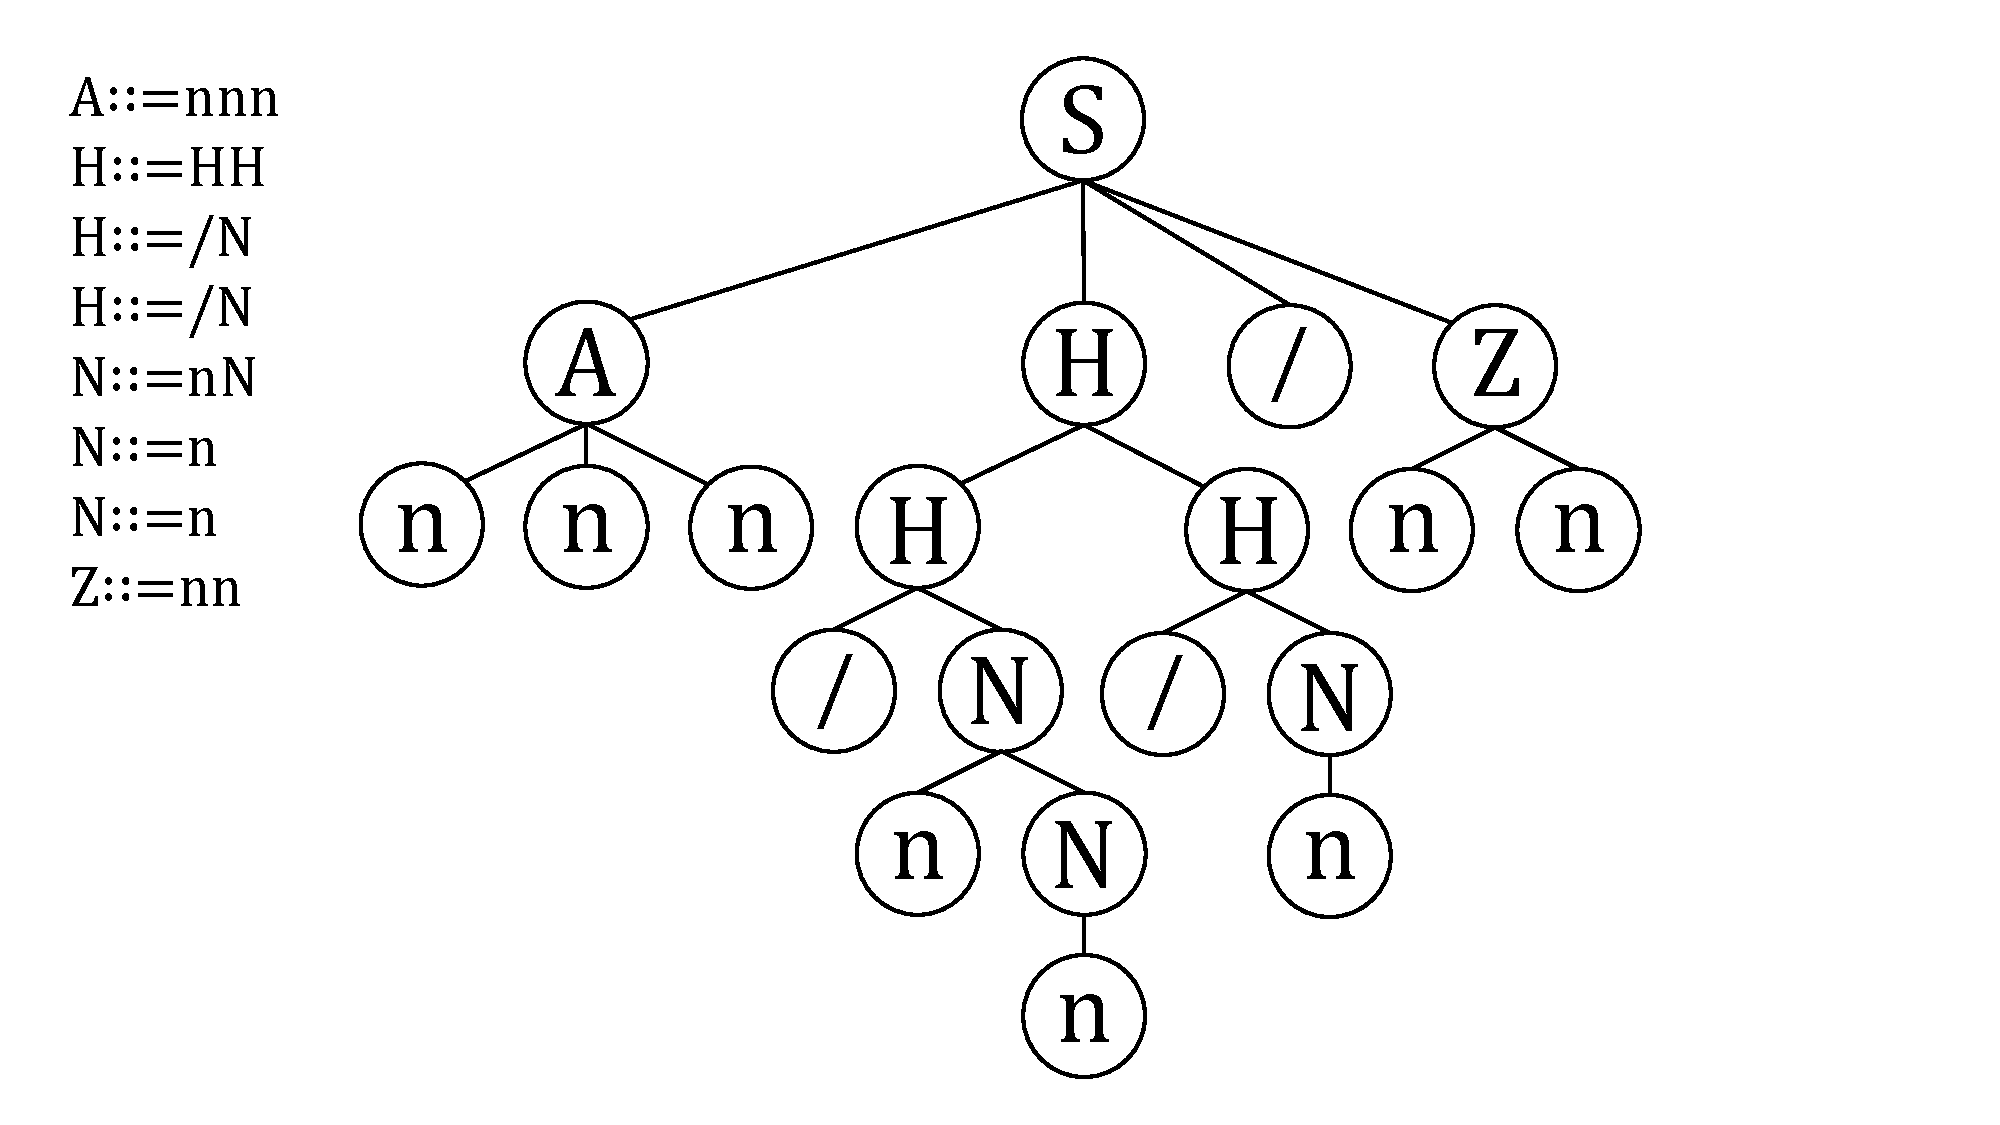
\includegraphics[width = 0.8\textwidth]{resources/Fig14_1.pdf}
      \end{figure} \par
      \vspace{-1cm}
      \begin{figure}[H]
        \centering
        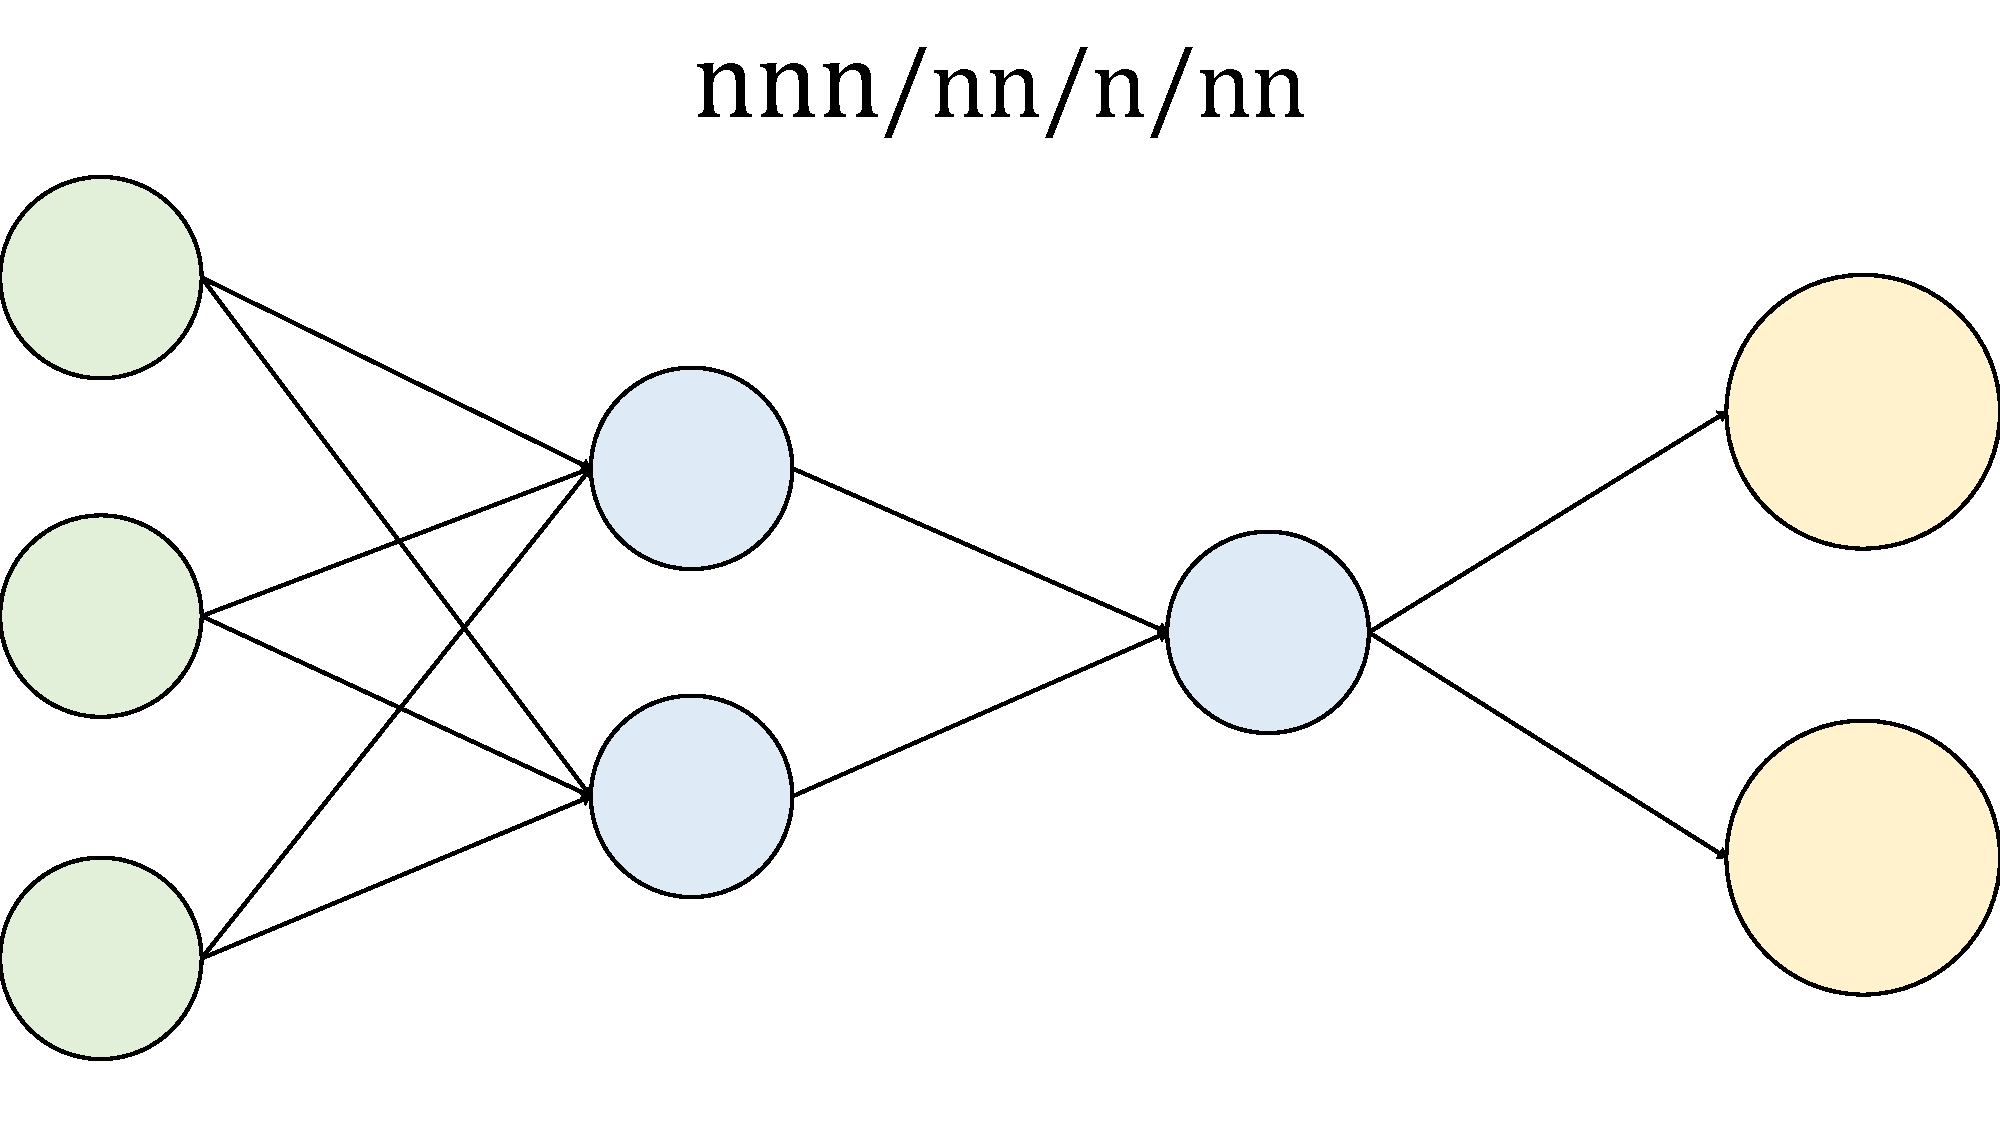
\includegraphics[width = 0.55\textwidth]{resources/Fig14_2.pdf}
        \caption{Individuo de ejemplo generado por la Eq. \ref{eq:3} y su decodificación en la arquitectura neuronal correspondiente.}
        \label{fig:14}
      \end{figure} \par
      En la Fig. \ref{fig:14} se muestra un individuo que se ha generado con la gramática de la Eq. \ref{eq:3} y sus reglas de producción en orden de aplicación, donde la cantidad de neuronas de entradas es $I = 3$ y la cantidad de neuronas de salida es $O = 2$. También se muestra la palabra que codifica el árbol y su decodificación como arquitectura neuronal. \par
      Esta gramática permite, por tanto, la construcción de arquitecturas de redes neuronales con varias capas ocultas. Como estas redes están totalmente conectadas, crea palabras fáciles de interpretar y de decodificar, sin preocuparse sobre las conexiones entre las capas y entre las neuronas. Sin embargo, la gramática no permite la creación de estructuras neuronales parcialmente conectadas. \par
      La gramática base mostrada en la Eq. \ref{eq:3} no permite añadir funciones de activación a cada capa, aunque puede ser fácilmente modificada para incluirlas, sustituyendo el separador de capa $/$ por un símbolo no terminal que deriva en una función de activación $f_i$. Esta modificación se puede ver en la gramática de la Eq. \ref{eq:4}. \par
    \begin{align*}
      G_{I\thinspace O\thinspace \mathbb{F}} &= (S, \Sigma_{N}, \Sigma_{T}, P_{I\thinspace O\thinspace \mathbb{F}}) \label{eq:4}\tag{4} \\
      \Sigma_{N} &= \{S, A, H, Z, N, F\} \\
      \Sigma_{T} &= \{n, f_1, f_2, ..., f_{\Phi}\} \\
      P_{I\thinspace O\thinspace \mathbb{F}} &= \{ \\
      &S ::= AHFZ \\
      &A ::= n^I \\
      &H ::= HH | FN \\
      &Z ::= n^O \\
      &N ::= nN | n \\
      &F ::= f_1 | f_2 | ... | f_{\Phi} \\
      \}
      \end{align*}
  
  \newpage\cleardoublepage
  
  \chapter{\vspace{-3cm}{\LARGE 5. Planteamiento del problema}}
  \setcounter{figure}{14}
  \vspace{-1cm}
  La Programación Genética permite la resolución de problemas de búsqueda y de optimización donde las soluciones son programas informáticos. Por tanto, cada uno de los individuos que codifica una solución al problema representa un programa informático. La ampliación de esta técnica con Gramáticas Libres de Contexto permite asegurar la generación de individuos sintácticamente válido, ahorrando tiempo y esfuerzo en reparar aquellos individuos no válidos que se dan sin la inclusión de estas gramáticas. \par
  La existencia de una gramática que permite generar Redes de Neuronas Artificiales establece una alternativa al problema de encontrar la mejor arquitectura que se adapte a un problema determinado. Anteriormente, este problema se abordaba con el conocimiento experto y la prueba y error. \par
  En el proceso evolutivo, cada individuo representa una red de neuronas, por lo que tiene que ser entrenado para la obtención de su grado de adaptación. Este proceso de entrenamiento se utiliza para cada nuevo individuo de la población. \par
  \begin{figure}[H]
    \centering
    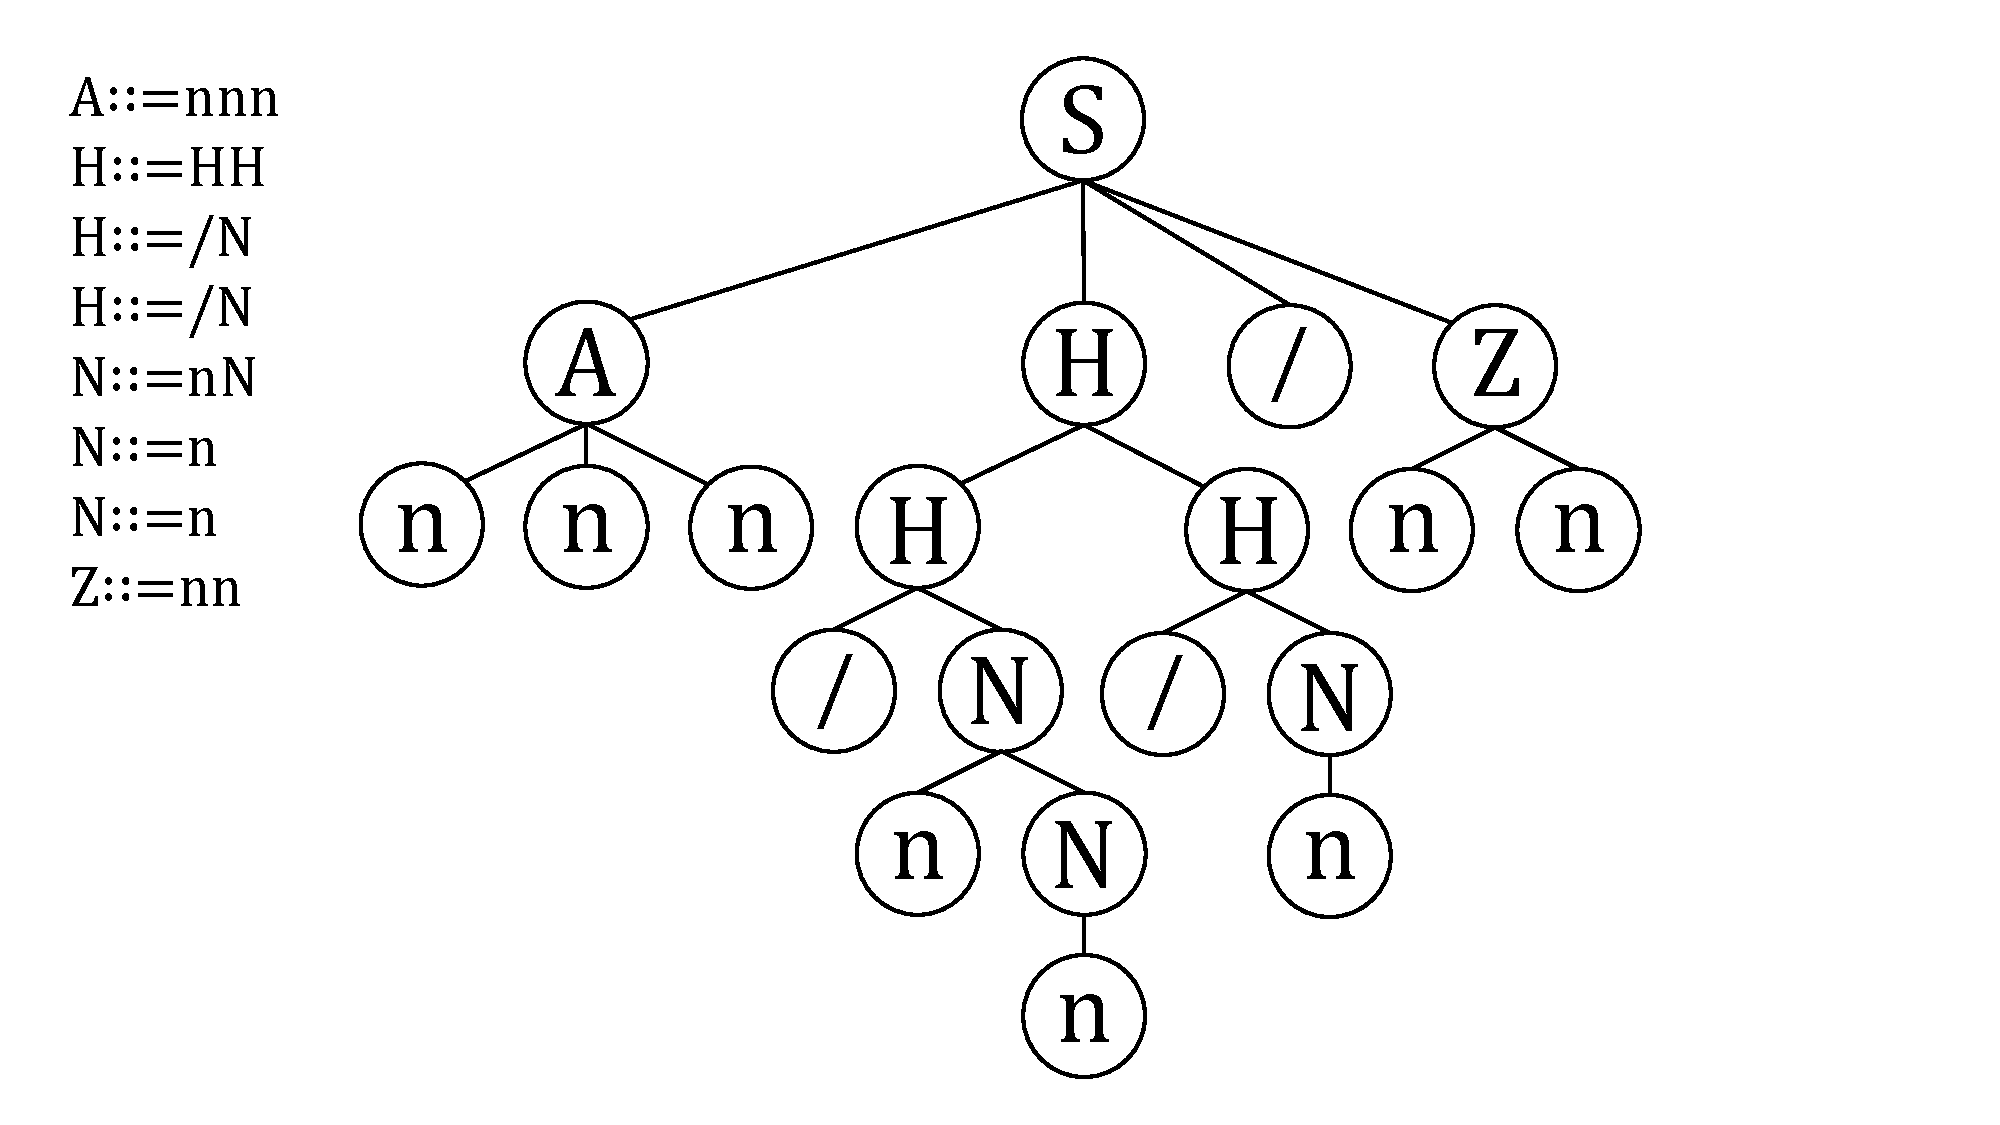
\includegraphics[width = 1\textwidth]{resources/Fig15.pdf}
    \caption{Proceso evolutivo aplicado al ámbito de creación de Redes de Neuronas Artificiales.}
    \label{fig:15}
  \end{figure} \par
  Este proceso evolutivo de construcción de redes neuronales se observa en la Fig. \ref{fig:15}. Comienza a partir de un conjunto de datos, para poder generar la gramática en base al número de entradas y de salidas. Se utiliza esta gramática para generar la población inicial, que se evalúa en primera instancia y se comprueba si la población generada cumple alguna condición de parada. Si es así, finaliza. En caso negativo, itera aplicando los operadores genéticos. \par
  Para problemas pequeños, el entrenamiento de estas redes requiere de poco tiempo. A medida que los datos y la arquitectura neuronal adquieren mayor dimensión, la demora en el entrenamiento comienza a ser significativa. Este aspecto hace que esta metodología pierda eficiencia cuando realmente es más necesaria; en el ámbito del Deep Learning, donde hay una gran cantidad de información y las arquitecturas neuronales deben ser profundas para ajustarse a los datos adecuadamente. \par
  Se propone en este Trabajo de Fin de Máster la reducción de la complejidad temporal mediante la parada prematura del entrenamiento de los individuos a la hora de calcular su grado de adaptación. Hay varios elementos que son clave en el entrenamiento de las Redes de Neuronas Artificiales: \par
  \begin{itemize}
    \item Tamaño del lote (\emph{batch size}). El entrenamiento por lotes (o mini-lotes) es muy común en las redes de neuronas. Un lote es un subconjunto de los datos de entrenamiento.
    \item Época (\emph{epoch}). Es la presentación de todos los lotes de entrenamiento a la red para el ajuste de sus pesos.
    \item Iteración de entrenamiento. Proceso mediante el cual se presenta a la red neuronal un lote y se ajustan sus pesos. El número total de iteraciones que habrá en una época se corresponde con la cantidad de lotes.
  \end{itemize} \par
  La parada prematura del entrenamiento se establece como una reducción en el número de épocas de entrenamiento de cada individuo. Se quiere mostrar si los resultados obtenidos en términos de la precisión de las redes de neuronas solución de un programa genético con un entrenamiento parcial de los individuos codificados como Redes de Neuronas Artificiales son comparables a un programa genético con un entrenamiento total, lo que supondría un ahorro de tiempo y esfuerzo computacional elevado. \par
  Ambos procesos se realizan de forma síncrona: mientras se entrena la red de neuronas codificada por un nuevo individuo de la población para calcular su grado de adaptación, el sistema evolutivo queda suspendido a la espera de que finalice el proceso de entrenamiento, ya sea de forma total o parcial.
    
  \chapter{\vspace{-3cm}{\LARGE 6. Solución propuesta}}
  \setcounter{figure}{16}
  \vspace{-1cm}
  La solución propuesta para este trabajo consiste en: \par
  \begin{itemize}
    \item Implementación de un Programa Genético Guiado por Gramáticas que construya Redes de Neuronas Artificiales y donde el grado de adaptación de los individuos que representan redes neuronales se calcule en base a su error en el proceso de entrenamiento.
    \item Búsqueda de conjuntos de datos, en concreto 3, que tengan tamaños incrementales, a fin de probar el mecanismo evolutivo con la mayor variedad posible.
    \item Realizar dos ejecuciones para cada conjunto de datos; una primera ejecución realizando el entrenamiento completo de los individuos y una segunda, con una parada prematura del entrenamiento.
  \end{itemize} \par
  Para realizar el trabajo, se ha desarrollado el código fuente de una librería utilizando el lenguaje de programación \emph{R}. Se ha decidido implementar esta librería por el hecho de que no había ningún otro paquete en este lenguaje que permitiese ejecutar programas genéticos con gramáticas definidas por un usuario. \par
  \section*{\Large 6.1. Generación de individuos y operadores genéticos}
  La implementación de esta librería consiste en el desarrollo de todos los operadores genéticos que constituyen el ciclo evolutivo, además del resto de elementos que intervienen en él.  \par
  El algoritmo para la creación de los individuos que se evolucionan a lo largo del programa que se ha seleccionado es el aleatorio, es decir, que siguiendo la gramática mostrada en la Eq. \ref{eq:3}, los individuos se generan a partir de reglas de producción aleatorias y sin una profundidad máxima determinada.\par
  El operador de selección elegido es por torneo, que escoge al azar tantos individuos de la población como el tamaño deseado, en este caso sin reemplazamiento, y se selecciona al mejor grupo de entre los elegidos. Este operador permite que haya un equilibrio entre exploración y explotación. Su funcionamiento puede verse en el algoritmo 1. \par\par
  El operador de cruce que se ha elegido es el de Whigham. En él, se selecciona un símbolo aleatorio del conjunto de símbolos no terminales del primer progenitor, y, a continuación, de los símbolos no terminales del segundo progenitor se selecciona uno aleatorio de entre aquellos idénticos al elegido. Esta decisión es adecuada ya que establece un equilibrio entre exploración y explotación. \par
  La implementación se aproxima en el algoritmo 2. \par
  \begin{algorithm}[H]
    \caption{Algoritmo del operador de selección por torneo}\label{selop}
    \begin{algorithmic}[1]
      \Function{selection}{$p, n$} \Comment{\textit{p} = Población, \textit{n} = Tamaño}
        \State $matting\_pool \gets \thinspace $[ ]
        \State $i \gets \thinspace $0
        \While{$i < \textnormal{round}(n/2)$}
          \State $seleccionados \gets \thinspace $sample(p, n)
          \State $p \gets \thinspace $remove(seleccionados, p)
          \State order(\textit{seleccionados})
          \State $mejores \gets \thinspace $head(\textit{seleccionados}, round(\textit{n}/2))
          \State append(\textit{matting\_pool}, \textit{mejores})
          \State $i \gets \thinspace $\textit{i} + 1
        \EndWhile
        \State \Return \textit{matting\_pool}
      \EndFunction
    \end{algorithmic}
  \end{algorithm} 
  \begin{algorithm}[H]
    \caption{Algoritmo del operador de cruce de Whigham}\label{cruzop}
    \begin{algorithmic}[1]
      \Function{crossover}{$f$} \Comment{\textit{f} = Progenitores}
        \State $no\_terminales1 \gets \thinspace $extraer(\textit{f[0]}) \Comment{Extraer símbolos no terminales}
        \State $no\_terminales2 \gets \thinspace $extraer(\textit{f[1]})
        \State $simbolo1 \gets \thinspace $sample(\textit{no\_terminales1}, 1)
        \State $simbolo2 \gets \thinspace $sample.choice([\textit{n} for \textit{n} in \textit{no\_terminales2} if \textit{n} == \textit{simbolo1}])
        \State $d \gets \thinspace $[] \Comment{Descendientes}
        \State $d[0] \gets \thinspace $replace(\textit{f[1]}, \textit{f[0]}, \textit{simbolo1}, \textit{simbolo2})
        \State $d[1] \gets \thinspace $replace(\textit{f[0]}, \textit{f[1]}, \textit{simbolo2}, \textit{simbolo1})
        \State \Return \textit{d}
      \EndFunction
    \end{algorithmic}
  \end{algorithm}
  La mutación se lleva a cabo de forma aleatoria tal y como se generan los individuos. Cuando un individuo se ve afectado por una mutación, se escoge un nodo no terminal de forma aleatoria y se sustituye por una derivación. Como la gramática utilizada favorece a las arquitecturas pequeñas al disminuir la probabilidad de recursión a medida que se llevan a cabo otras, este algoritmo es adecuado. \par
  \begin{algorithm}[H]
    \caption{Algoritmo del operador de reemplazo por reducción elitista}\label{reemop}
    \begin{algorithmic}[1]
      \Function{replacement}{$p, d$} \Comment{\textit{p} = Población, \textit{d} = Descendientes}
        \State $tamano \gets \thinspace $length(\textit{p})
        \State $total \gets \thinspace $merge(\textit{p}, \textit{d})
        \State $total\_ordenado \gets \thinspace $order(\textit{total})
        \State $p \gets \thinspace $head(\thinspace{total\_ordenado}, \textit{tamano})
      \EndFunction
    \end{algorithmic}
  \end{algorithm}
  Finalmente, el operador de reemplazo que se ha escogido es por reducción elitista. En él, tras seleccionar a los individuos de la población que pasarán a formar parte del \emph{matting pool} y cruzarlos para conformar su descendencia, los progenitores, el resto de individuos y los descendientes, se juntan y posteriormente se seleccionan a los $\lambda$ mejores. \par
  \begin{figure}[H]
    \centering
    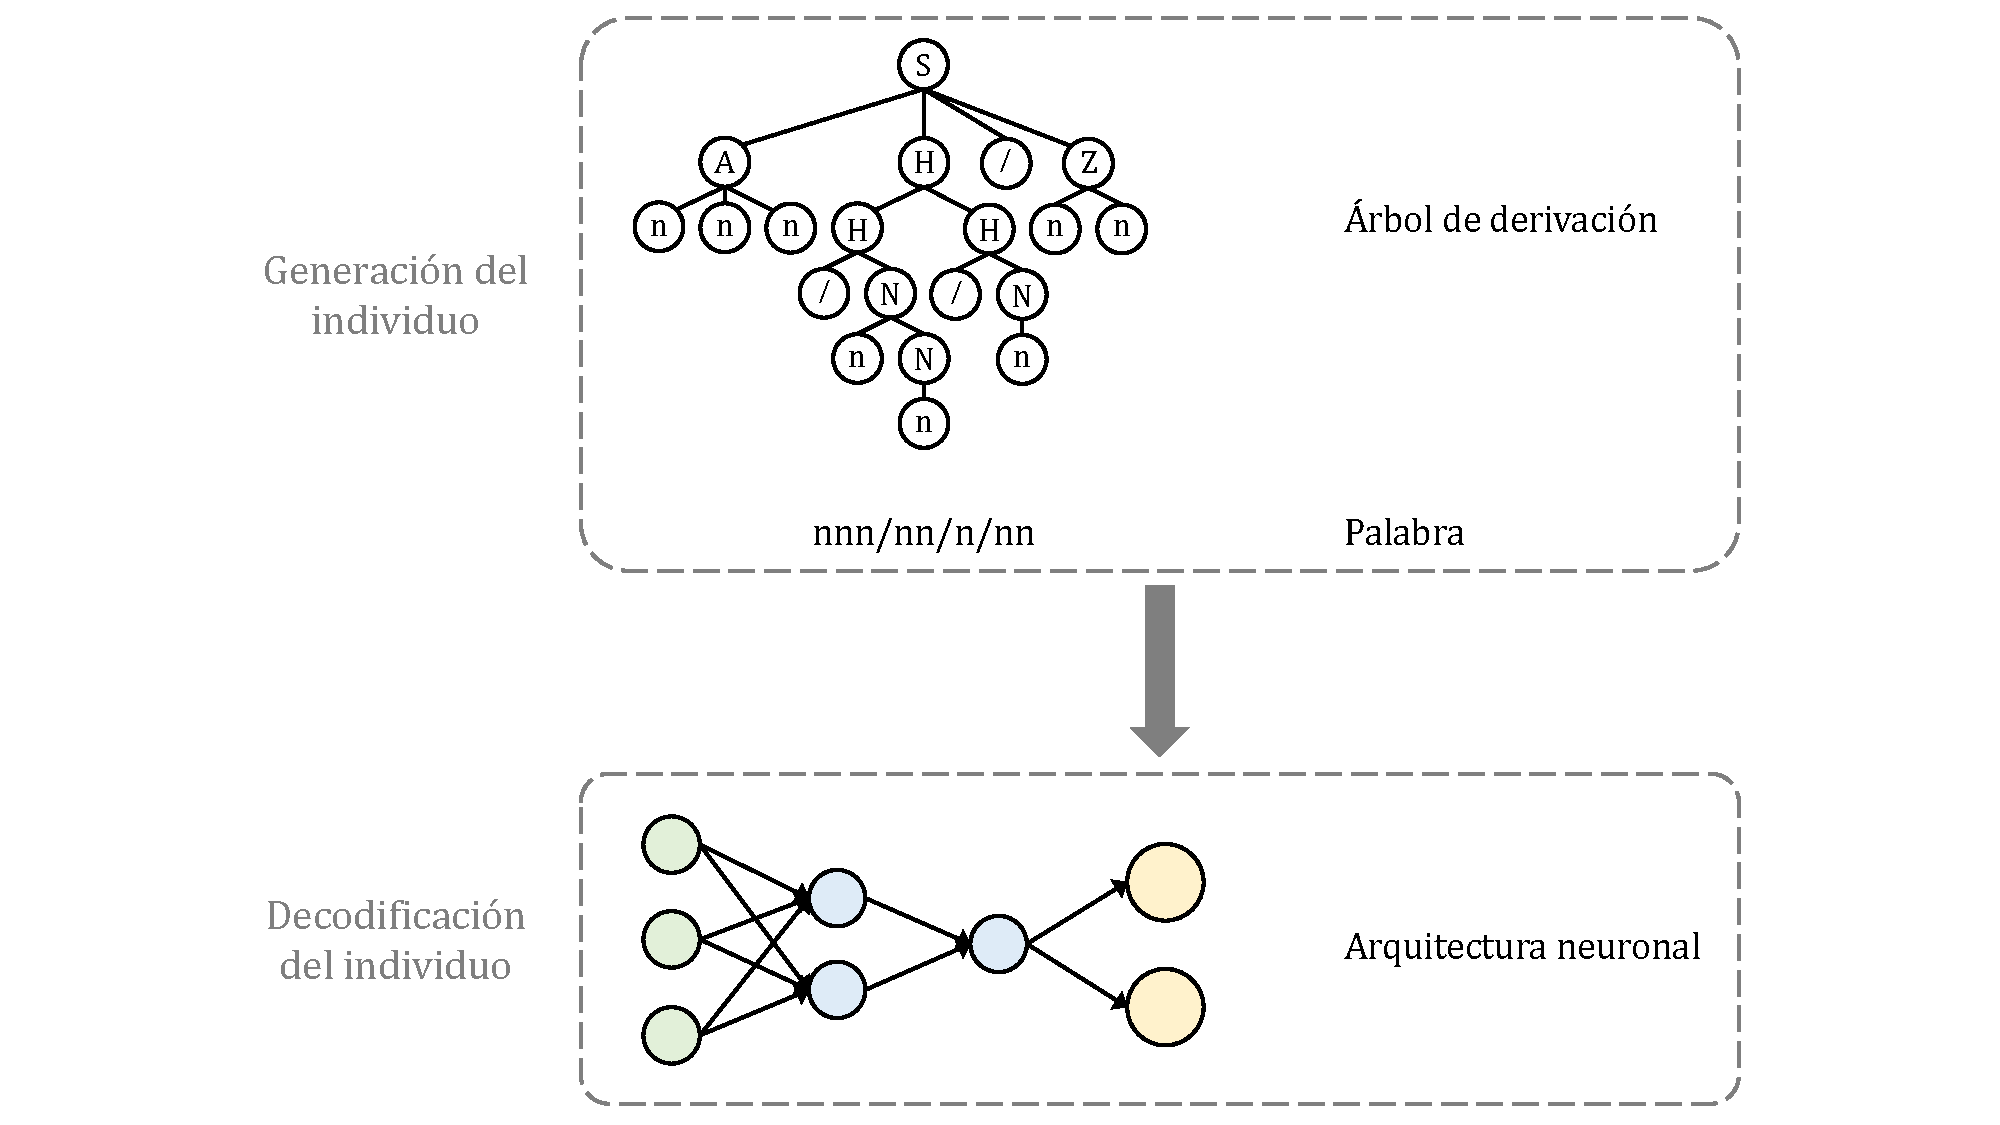
\includegraphics[width = 1\textwidth]{resources/Fig16_1.pdf}
  \end{figure} \par
  \vspace{-1cm}
  \begin{figure}[H]
    \centering
    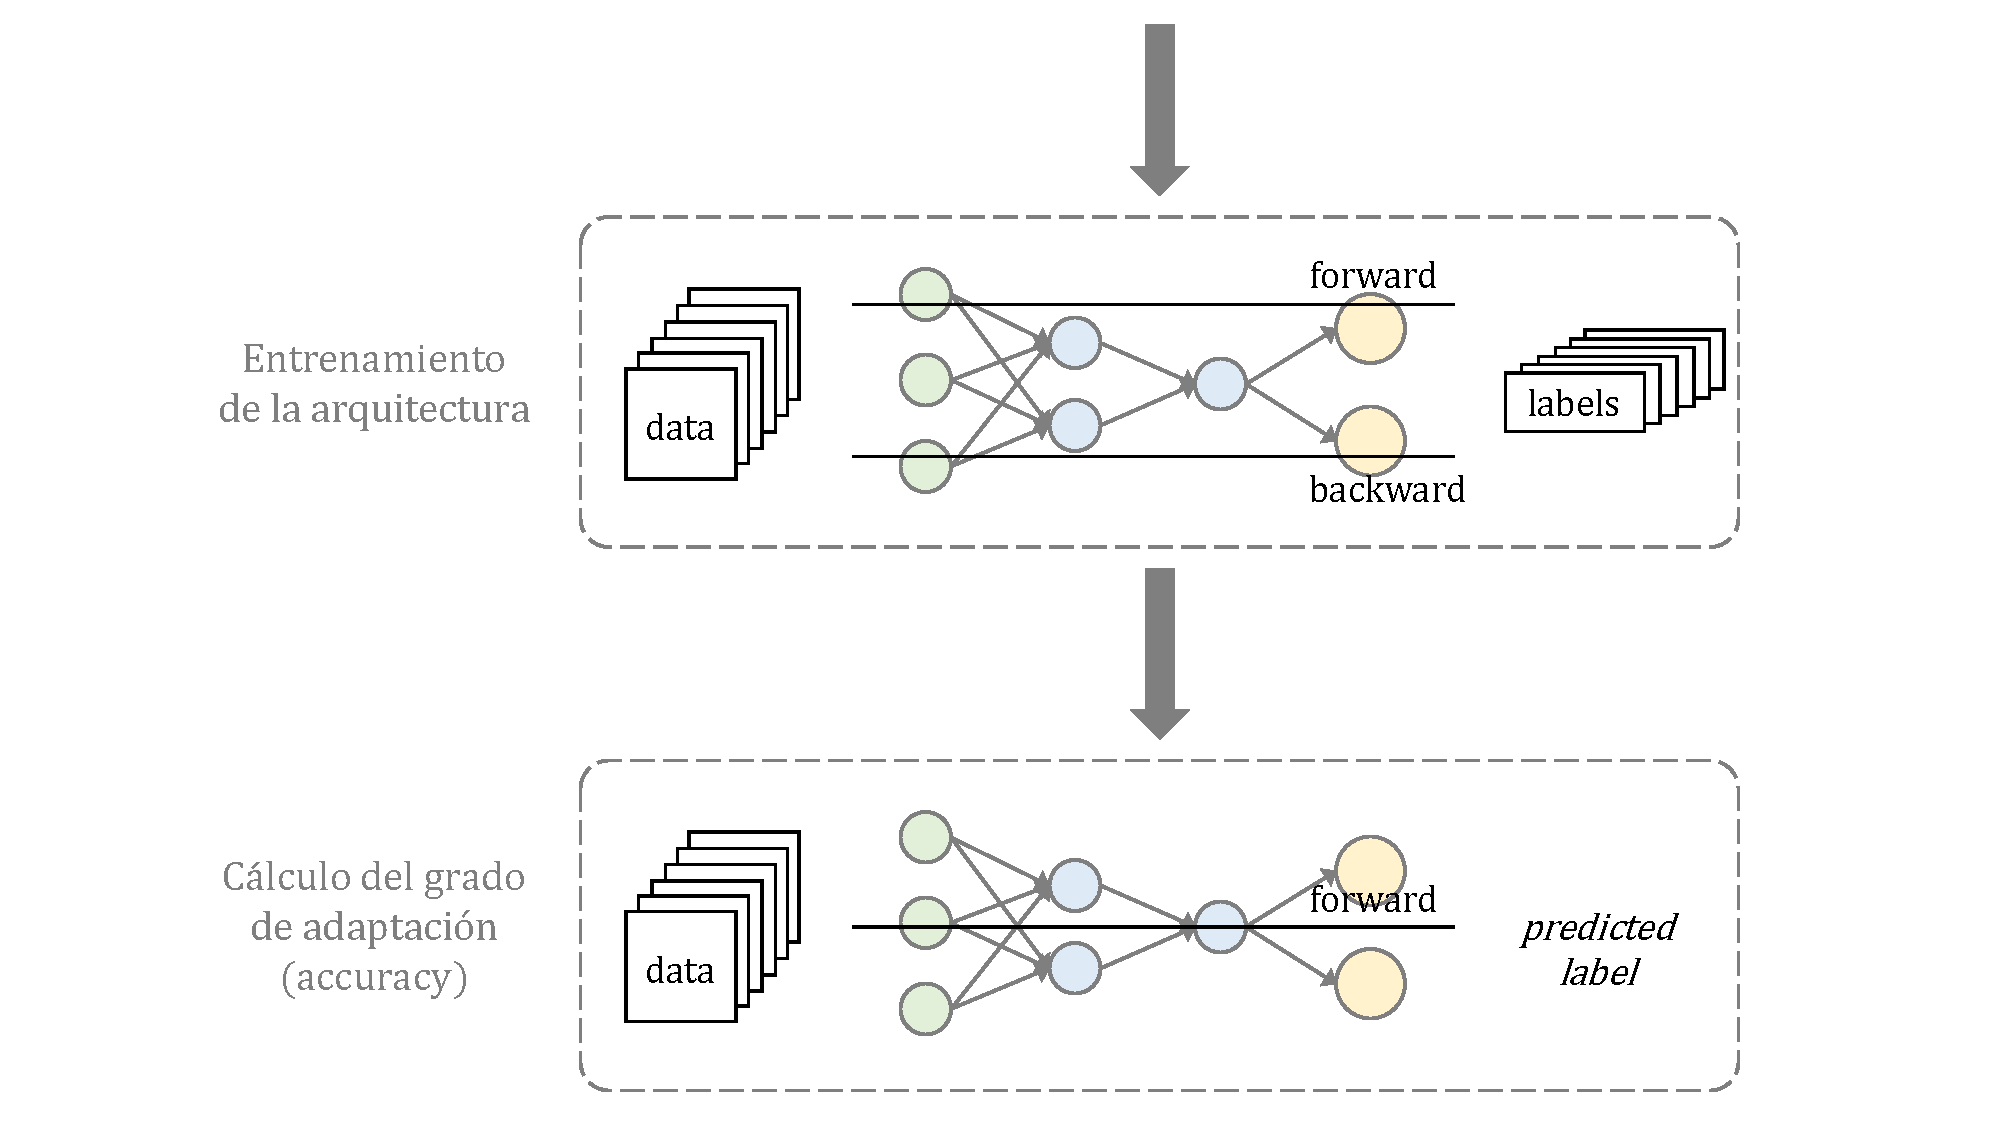
\includegraphics[width = 1\textwidth]{resources/Fig16_2.pdf}
    \caption{Proceso de evaluación de un individuo.}
    \label{fig:16}
  \end{figure} \par
  \section*{\Large 6.2. Entrenamiento de individuos}
  Los individuos codifican arquitecturas neuronales gracias a la gramática utilizada. En el proceso evolutivo, interviene el proceso de evaluación de los individuos, que consiste en la decodificación, entrenamiento y cálculo de la precisión de los mismos. \par
  Este proceso puede verse en el diagrama de la Fig. \ref{fig:16}. \par
  Para el entrenamiento de los individuos se ha utilizado la librería de R \emph{Keras}, ya que permite la parametrización avanzada de las características del proceso, como las funciones de activación de cada neurona de la red, el número de épocas o un parámetro para detener el proceso en caso de sobreentrenamiento. \par
  La implementación del entrenamiento se puede visualizar en el algoritmo 4. \par
  \begin{algorithm}[H]
    \caption{Algoritmo de entrenamiento}\label{entren}
    \begin{algorithmic}[1]
      \Function{train}{$d, data, params$} \Comment{\textit{d} = Individuo}
        \State $palabra \gets \thinspace $toString(\textit{d}) \Comment{Extraer la palabra}
        \State $arquitectura \gets \thinspace $extraer(\textit{palabra})
        \State $train, test, val \gets \thinspace $split(\textit{data})
        \State $modelo \gets \thinspace $keras::train(\textit{arquitectura}, \textit{train}, \textit{val}, \textit{params})
        \State $accuracy \gets \thinspace $keras::predict(\textit{modelo}, \textit{test})
        \State \Return \textit{accuracy}
      \EndFunction
    \end{algorithmic}
  \end{algorithm}
  Este algoritmo es idéntico según se trate de un entrenamiento parcial o de uno total. La diferencia entre los dos modos residirá en el número de épocas que vayan a intervenir en el proceso. \par
  Los parámetros de entrenamiento que se han utilizado son los siguientes: \par
  \begin{itemize}
    \item Tamaño del lote. El tamaño del lote que se ha seleccionado ha sido de 64 elementos, independientemente del dataset y de si el entrenamiento es parcial o total.
    \item Épocas. El número de épocas es el único elemento que difiere según se trate de un entrenamiento parcial o total. Para los entrenamientos totales, se utiliza un número de épocas que sobrepasa el máximo necesario, pero como el algoritmo cuenta que mecanismos que impiden que haya sobreentrenamiento, el proceso se detiene antes. Para entrenamientos totales, el número de épocas utilizado es, para conjuntos de datos inferiores a 200 instancias, 100 épocas, y para conjuntos mayores, un tercio del número de instancias menos el producto de las variables predictoras y las de clase, según puede verse en la Eq. \ref{eq:5}.
    \begin{align*}
      \textnormal{número épocas} = \left\{ \begin{array}{lcc} \label{eq:5}\tag{5}
             100 &   si  & N < 200 \\
             \\ \frac{N}{3} - (E \cdot S) &  si & N \geq 200
             \end{array}
      \right.
    \end{align*}
    donde $N$ es el número de instancias del conjunto de datos, $E$ es el número de variables de entrada y $S$ es el número de variables de salida. Para entrenamientos parciales, la primera aproximación en la que se pensó fue en el corte entre el error y el tiempo en la curva de entrenamiento, de tal forma que llegaría, se supone, un punto en el que para disminuir el error una cantidad pequeña, se requeriría una carga de tiempo grande, por lo cual se podría parar en ese punto. Sin embargo, para conjuntos de datos pequeños y que entrenan rápido esto no se cumple, ya que también está condicionado por la arquitectura, por lo que sería un número dinámico dependiente del modelo, restando consistencia a los resultados. El número de épocas deseado para el entrenamiento parcial es de, para conjuntos inferiores a 3500 instancias, el producto entre sus entradas y sus salidas más una unidad, y para conjuntos de más instancias, el doble del cociente entre el producto entre la entrada, la salida y 10 y el número de instancias, según puede verse en la Eq. \ref{eq:6}.
    \begin{align*}
      \textnormal{número épocas} = \left\{ \begin{array}{lcc} \label{eq:6}\tag{6}
             (E \cdot S) + 1 &   si  & N < 3500 \\
             \\ \frac{E \cdot S \cdot 10}{N} \cdot 2 &  si & N \geq 3500
             \end{array}
      \right.
    \end{align*}
    donde $N$ es el número de instancias del conjunto de datos, $E$ es el número de variables de entrada y $S$ es el número de variables de salida.
    \item Control del sobreentrenamiento. Se ha establecido un mecanismo que controla el sobreentrenamiento de la red. El procedimiento que se sigue se lleva a cabo mientras la red está entrenando, de tal forma que en cada época se mide el error de la red con el subconjunto de validación. Si el error aumenta durante un 10\% de las épocas seguidas, el entrenamiento se detiene. En caso contrario, sigue entrenando. Este mecanismo es especialmente necesario en los entrenamientos totales, ya que en los parciales la inmensa mayoría de los individuos entrenan sin sobreentrenar.
    \item Tasa de aprendizaje dinámica. Junto con el control de entrenamiento anterior, la posibilidad de contar con una tasa de aprendizaje dinámica evita el sobreentrenamiento y también el estancamiento de las redes. Se establece también un mecanismo que, si el modelo se estanca durante un 5\% de las épocas seguidas, disminuya la tasa de aprendizaje en un 15\%, y si el modelo sobreentrena durante un 5\% de las épocas seguidas, la aumente un 20\%. De esta forma se facilita que el entrenamiento sea dinámico, permitiendo que el parámetro de aprendizaje de la red se adapte según el estado de los pesos y del algoritmo de aprendizaje, y evitando que el control del sobreentrenamiento se aplique siempre.
    \item División del conjunto de datos en entrenamiento, validación y test. Para todos los conjuntos de datos, se ha extraído un subconjunto de entrenamiento (con, aproximadamente, un 70\% de instancias), de validación (con, aproximadamente, un 20\% de instancias) y de test (con las restantes).
    \item Pesos de clase. Si bien la mayoría de los conjuntos de datos cuentan con, aproximadamente, un número semejante de instancias de cada clase, en otros casos sucede que hay una desproporción en su conteo. En tal caso, es necesario que estas clases más mayoritarias tengan un menor peso en el cálculo del error. Este cálculo se refleja en la Eq. \ref{eq:7}.
    \begin{align*}
      w_{C_i} = \frac{1 - \frac{N_{C_i}}{N}}{\sum_{j=1}^{m}1 - \frac{N_{C_j}}{N}} \label{eq:7}\tag{7}
    \end{align*}
    donde $w_{C_i}$ es peso que se le asocia a la clase $C_i$ en el cálculo del error en cada época, $N_{C_i}$ es el número de instancias del conjunto de datos etiquetadas con la clase $C_i$ y el sumatorio es la suma de las proporciones inversas de las clases en el conjunto de datos.
  \end{itemize} \par
  El proceso de entrenamiento concluye con el cálculo del \emph{accuracy} con el subconjunto de entrenamiento. La justificación de utilizar este subconjunto y no otros reside en que si la red tiene un mal desempeño con estos datos, también lo tendrá con los de validación y test. Por tanto, aquellos individuos con un \emph{accuracy} malo en entrenamiento, son descartables por su bajo grado de adaptación.
  \section*{\Large 6.3. Programa genético}
  El programa genético sigue el ciclo evolutivo y se ejecutará un total de 80 veces, para entrenamientos totales y parciales. \par
  Para cada ejecución, se almacena el modelo entrenado de cada individuo, así como su historial de entrenamiento, con la variación del error y del \emph{accuracy} para cada época. \par
  \begin{algorithm}[H]
    \caption{Algoritmo del programa genético}\label{entren}
    \begin{algorithmic}[1]
      \Function{genetic\_program}{$n, cfg, d, p$} \Comment{\textit{n} = Tamaño, \textit{cfg} = Gramática, \textit{d} = Datos, \textit{p} = Parámetros}
        \For{\texttt{$i \gets \thinspace $1 to 80}}
          \State $poblacion \gets \thinspace $generar(\textit{n}, \textit{cfg})
          \For{\texttt{$j \gets \thinspace $1 to n}}
            \State $poblacion[j] \gets \thinspace $train(\textit{poblacion[j]}, d, p)
          \EndFor
          \While{!condicion\_parada(\textit{poblacion})}
            \State $progenitores \gets \thinspace $selection(\textit{poblacion}, \textit{round(n/2)})
            \State $descendencia \gets \thinspace $crossover(\textit{matting\_pool})
            \State $m \gets \thinspace $length(\textit{descendencia})
            \For{\texttt{$j \gets \thinspace $1 to m}}
              \State $descendencia[j] \gets \thinspace $train(\textit{descendencia[j]}, d, p)
            \EndFor
            \State $\textit{descendencia}, \textit{progenitores} \gets \thinspace $mutation(\textit{descendencia}, \textit{progenitores})
            \State $poblacion \gets \thinspace $replacement(\textit{poblacion}, \textit{descendencia})
          \EndWhile
          \State $solucion \gets \thinspace $obtener\_solucion(\thinspace{poblacion})
          \State guardar\_resultados(\textit{solucion})
        \EndFor
        \State analizar\_resultados
      \EndFunction
    \end{algorithmic}
  \end{algorithm} \par
  El procedimiento que sigue el programa genético se puede ver en el algoritmo 5. \par
  La cantidad de individuos seleccionados, para un tamaño de la población es del 20\%, es decir, de 6 progenitores para conformar una descendencia de 6 individuos (cada pareja de progenitores genera una pareja de descendientes). \par
  Sobre los individuos seleccionados y sus descendientes se aplica la mutación con una probabilidad del 5\%, que a lo l \par
  El tiempo de ejecución depende directamente del número de épocas, de la dimensión de los datos y de si el sistema que lo ejecuta cuenta con una unidad de procesamiento gráfico. Para dimensiones pequeñas y 80 ejecuciones, la diferencia entre el uso de procesamiento gráfico y el no uso es prácticamente nula. En el caso opuesto, la red no entrenará a menos que cuente con una unidad de procesamiento gráfico que lo permita. \par
  En el caso concreto de este trabajo, cuando la dimensión de los datos superaba las 35.000 instancias, las redes nunca llegaron a entrenar totalmente. \par
  Por lo tanto, si bien este programa genético funciona de forma adecuada, la máquina es totalmente influyente en su éxito o fracaso, de tal forma que sin una potencia de cómputo adecuada, habrá problemas que sean irresolubles, al menos con el entrenamiento total. Con el entrenamiento parcial, al reducir el número de épocas de forma considerable, es posible llegar a realizar una ejecución completa.
  % TOTAL: 100 IRIS, 500 CAR
  % PARCIAL: 13 IRIS, 20 CAR, 300 OCEAN PROXIMITY
  
  \chapter{\vspace{-3cm}{\LARGE 7. Resultados}}
  
  \chapter{\vspace{-3cm}{\LARGE 8. Conclusiones y líneas futuras}}
  \vfill
  
  \begin{thebibliography}{00}
  \vspace{-1cm}
  \makeatletter
  \def\@biblabel#1{}
  \let\old@bibitem\bibitem
  \def\bibitem#1{\old@bibitem{#1}\leavevmode\kern-\bibindent}
  \makeatother
  
  \bibitem{Aizenberg2000} Aizenberg, I., Aizenberg, N.N. and Vandewalle, J.P.L. (2000). \emph{Multi-Valued and Universal Binary Neurons: Theory, Learning and Applications}.
  \bibitem{Banzhaf1998} Banzhaf, W., Poli, R., Schoenauer, M. and Fogarty, T.C. (1998). \emph{Genetic Programming}.
  \bibitem{Beni1989} Beni, G. and Wang, J. (1989). Swarm intelligence in cellular robotic systems. \emph{Proceedings5 of the NATO Advance Workshop on Robots and Biological Systems}. 102:703-712.
  \bibitem{Beni2004} Beni, G. (2004). From Swarm Intelligence to Swarm Robotics. \emph{International Workshop on Swarm Robotics}. 3342:1-9.
  \bibitem{Boyd2004} Boyd, S. and Vandenberghe, L. (2004). Convex Optimization. \emph{Cambridge University Press 2004}: 129.
  \bibitem{Box1957} Box, G.E.P. (1957). Evolutionary operation: A method for increasing industrial productivity. \emph{Journal of the Royal Statistical Society. Series C}. 6(2):81-101.
  \bibitem{Box1969} Box, G.E.P. and Draper, N.P. (1969). \emph{Evolutionary Operation. A method for Increasing Industrial Productivity}.
  \bibitem{Bremermann1962} Bremermann, H.J. (1962). Optimization through evolution and recombination. \emph{Self-Organizing Systems 1962}: 93-106.
  \bibitem{Chomsky1959} Chomsky, N. (1959). On Certain Formal Properties of Grammars. \emph{Information and Control}. 2(2):137-167.
  \bibitem{Couchet2006} Couchet, J. and Manrique, D. (2006). Crossover and mutation operations for grammar-guided genetic programming. \emph{Soft Computing}. 11(10):943-955.
  \bibitem{Couchet2007} Couchet, J., Manrique, D. and Porras, L. (2007). Grammar-Guided Neural Architecture Evolution. \emph{Bio-inspired Modeling of Cognitive Tasks}: 438-446.
  \bibitem{Cramer1985} Cramer, N.L. (1985). A representation for the Adaptive Generation of Simple Sequential Programs. \emph{Proceedings of the First International Conference on Genetic Algorithms and the Applications}: 183-187.
  \bibitem{Dhaeseleer1994} D'haeseleer, P. (1994). Context preserving crossover in genetic programming. \emph{Proceedings of the First IEEE Conference on Evolutionary Computation}. 1:256-261.
  \bibitem{Dantzig1990} Dantzig, G.B. (1990). Origins of the simplex method. \emph{A history of scientific computing}, pages 141-151.
  \bibitem{Darwin1859} Darwin, C. (1859). \emph{On the Origin of Species by Means of Natural Selection, or Preservation of Favoured Races in the Struggle for Life}. 
  \bibitem{deAraujo2014} De Araujo, A.F. and Tavares, J.M.R.S. (2014). An Artificial Life Model for Image Enhancement. \emph{15th International Conference on Experimental Mechanics}. 41(13):5892-5906.
  \bibitem{Deb2002} Deb, K., Agarwal, S., Pratap, A. and Meyarivan, T. (2002). A Fast and Elitist Multiobjective Genetic Algorithm: NSGA-II. \emph{IEEE Transactions on Evolutionary Computation}. 6(2):128-197.
  \bibitem{Farmer1986} Farmer, J.D., Packard, N.H. and Perelson, A.S. (1986). The Immune System, Adaptation, and Machine Learning. \emph{Physica D: Nonlinear Phenomena}. 22(1): 187-204.
  \bibitem{Fogel1966} Fogel, L.J., Owens, A.J. and Walsh, M.J. (1966). \emph{Artificial Intelligence through Simulated Evolution}.
  \bibitem{Fraser1957} Fraser, A.S. (1957). Simulation of Genetic Systems by Automatic Digital Computers. \emph{Australian journal of biological sciences}. 10:484-499.
  \bibitem{Friedberg1958} Friedberg, R.M. (1958). A learning machine: part I. \emph{IBM Journal of Research and Development}. 2(1):2-13.
  \bibitem{Friedberg1959} Friedberg, R.M., Dunham, B. and North, J.H. (1959). A learning machine: part II. \emph{IBM Journal of Research and Development}. 3(3):282-287.
  \bibitem{Fukushima1975} Fukushima, K. (1975). Cognitron: A self-organizing multilayered neural network. \emph{Biological Cybernetics}. 20(3):121-136.
  \bibitem{GarciaArnau2007} García-Arnau, M., Manrique, D., Ríos, J. and Rodríguez-Patón, A. (2007). Initialization method for grammar-guided genetic programming. \emph{Research and Development in Intelligent Systems XXIII}: 32-44.
  \bibitem{Geem2001} Geem, Z.W., Kim, J.H. and Loganathan, G.V. (2001) A New Heuristic Optimization Algorithm: Harmony Search. \emph{Simulation}, 76(2):60-68.
  \bibitem{Goldberg1989} Goldberg, D.E. (1989). \emph{Genetic Algorithms in Search, Optimization \& Machine Learning}.
  \bibitem{Grefenstette1985} Grefenstette, J.J. (1985). \emph{Proceedings of the First International Conference on Genetic Algorithms and the Applications} (Hillsdale, NJ: Lawrence Erlbaum).
  \bibitem{Grefenstette1987} Grefenstette, J.J. (1987). \emph{Proceedings of the Second International Conference on Genetic Algorithms and the Applications} (Hillsdale, NJ: Lawrence Erlbaum).
  \bibitem{Hassan2005} Hassan, R., Cohanim, B., de Weck, O. and Venter, G. (2005). A comparison of particle swarm optimization and the genetic algorithm. \emph{46th AIAA/ASME/ASCE/AHS/ASC Structures, Structural Dynamics and Materials Conference}.
  \bibitem{Hebb1949} Hebb, D.O. (1949). \emph{The Organization of Behavior}. (New York: Wiley).
  \bibitem{Holland1962} Holland, J.H. (1962). Nonlinear environments permitting efficient adaptation. \emph{Computer and Information Sciences II}: 147-164.
  \bibitem{Hopcroft1979} Hopcroft, J.E. and Ullman, J.D. (1979). Context-Free Grammars. \emph{Introduction to Automata Theory Languages and Computation}: 77-106.
  \bibitem{Hopfield1982} Hopfield, J.J. (1982). Neural networks and physical systems with emergent collective computational abilities. \emph{Proceedings of the National Academy of Sciences of the United States of America}. 79(8):2554-2558.
  \bibitem{Hu2014} Hu, T., Banzhaf, W. and Moore, J.H. (2014). The effects of recombination of phenotypic exploration and robustness in evolution. \emph{Artificial Life}. 20(4):457-470.
  \bibitem{Klopf1972} Klopf, A.H. (1972). Brain Function and Adaptive Systems - A Heterostatic Theory. \emph{Air Force Cambridge Research Laboratories}.
  \bibitem{Kohonen1982} Kohonen, T. (1982). Self-Organized Formation of Topologically Correct Feature Maps. \emph{Biological Cybernetics}. 43:59-69.
  \bibitem{Koza1988} Koza, J.R. (1988). Non-Linear Genetic Algorithms for Solving Problems. \emph{University States Patent 4935877}.
  \bibitem{Koza1992} Koza, J.R.(1992). \emph{Genetic Programming: On the Programming of Computers by Means of Natural Selection}  (Cambridge, MA: MIT Press).
  \bibitem{Koza1996} Koza, J.R., Goldberg, D.E., Fogel, D.B. and Riolo, R.L. (1996). \emph{Genetic Programming 1996} (Cambridge, MA: MIT Press).
  \bibitem{Kosorukoff2001} Kosorukoff, A. (2001). Human based genetic algorithm. \emph{2001 IEEE International Conference on Systems, Man and Cybernetics. e-Systems and e-Man for Cybernetics in Cyberspace}: 3464-3469.
  \bibitem{Langton1986} Langton, C.G. (1986). Studying artificial life with cellular automata. \emph{Physica D: Nonlinear Phenomena}. 22(1):120-149.
  \bibitem{Manrique2018} Manrique, D., Barrios, D.R., Delgado, G.M. (2018). Multilayered neural architectures evolution for computing sequences of orthogonal polynomials. \emph{Annals of Mathematics and Artificial Intelligence}. 84(3):161-184.
  \bibitem{McCulloch1943} McCulloch, W.S. and Pitts, W.H. (1943) A Logical Calculus of the Ideas Immanent in Nervous Activity. \emph{Bulletin of Mathematical Biophysics}. 5:115-133.
  \bibitem{Minsky1969} Minsky, M.L. and Papert, S. (1969). \emph{Perceptrons: An Introduction to Computational Geometry} (Cambridge: MIT Press).
  \bibitem{Moscato1989} Moscato, P. (1989). On Evolution, Search, Optimization, Genetic Algorithms and Martial Arts - Towards Memetic Algorithms. \emph{Caltech Concurrent Computation Program}: 158-179.
  \bibitem{Nocedal1999} Nocedal, J. and Wright, S.J. (1999). Numerical optimization. \emph{Springer-Verlag}.
  \bibitem{Pezzella2008} Pezzella, F., Morganti, G. and Ciaschetti, G. (2008). A genetic algorithm for the Flexible Job-shop Scheduling Problem. \emph{Computers \& Operations Research}. 35(10):3202-3212.
  \bibitem{Poli1997a} Poli, R. and Langdon, W.B. (1997a). An experimental analysis of schema creation, propagation and disruption in genetic programming. \emph{Proc. of ICGA'97}.
  \bibitem{Poli1997b} Poli, R. and Langdon, W.B. (1997b). A new schema theory for genetic programming with one-point crossover and point mutation. \emph{Proc. of the Second On-line World Conference on Soft Computing in Engineering Design and Manufacturing}.
  \bibitem{Poli1998} Poli, R. and Langdon, W.B. (1998). A review of theoretical and experimental results on schemata in genetic programming. \emph{Proceedings of the First European Workshop on Genetic Programming}.
  \bibitem{Polya1945} Polya, G. (1945). How to Solve It. \emph{Princeton University Press 1945}.
  \bibitem{Rawlins1991} Rawlins, G.J.E. (1991). \emph{Foundations of Genetic Algorithms} (San Mateo, CA: Morgan Kaufmann).
  \bibitem{Rechenberg1965} Rechenberg, I. (1965). Cybernetic Solution Path of an Experimental Problem. \emph{Royal Aircraft Establishment Library Translation 1122}.
  \bibitem{Reynolds1994} Reynolds, R.G. (1994). An Introduction to Cultural Algorithms. \emph{Proceedings of the 3rd Annual Conference on Evolutionary Programming}: 131-139.
  \bibitem{Roberts1965} Roberts, L. (1965). Machine perception of 3D solids. \emph{Optical and Electro-Optical Information Processing}. 9:159-197.
  \bibitem{Rosenblatt1958} Rosenblatt, F. (1958). The Perceptron: A Probabilistic Model for Information Storage and Organization in The Brain. \emph{Psychological Review}. 65(6):386-408.
  \bibitem{Rosenblatt1962} Rosenblatt, F. (1962). \emph{Principles of Neurodynamics} (Washington: Spartan Books). 
  \bibitem{Rumelhart1986} Rumelhart, D.E., Hinton, G.E. and Williams, R.J. (1986). Learning internal representations by error propagation. \emph{Parallel Distributed Processing: Explorations in the Microstructure of Cognition}. 1:318-362.
  \bibitem{Rumelhart1986a} Rumelhart, D.E., Hinton, G.E. and Williams, R.J. (1986). Learning representations by back-propagating errors. \emph{Nature}. 323:533–536.
  \bibitem{Ryan1998} Ryan, C., Collins, J.J. and O'Neil, M. (1998). Grammatical Evolution: Evolving Programs for an Arbitrary Language. \emph{Proceedings of the First European Workshop on Genetic Programming}: 83-96.
  \bibitem{Samuel1959} Samuel, A.L. (1959). Some Studies in Machine Learning Using the Game of Checkers. \emph{IBM Journal of Research and Development}. 3(3):210-229.
  \bibitem{Schaffer1989} Schaffer, J.D. (1989). \emph{Proceedings of the Third International Conference on Genetic Algoritms and the Applications} (San Mateo, CA: Morgan Kaufmann).
  \bibitem{Schwefel1965} Schwefel, H-P. (1965). Kybernetische Evolution als Strategie der experimentellen Forschung in der Strömungstechnik.
  \bibitem{Storn1996} Storn, R. (1996). On the usage of differential evolution for function optimization. \emph{Biennial Conference of the North American Fuzzy Information Processing Society}: 519-523.
  \bibitem{Storn1997} Storn, R. and Price, K. (1997). Differential evolution - a simple and efficient heuristic for global optimization over continuous spaces. \emph{Journal of Global Optimization}. 11(4):341-359.
  \bibitem{Tackett1995} Tackett, W.A. (1995). Greedy Recombination and Genetic Search on the Space of Computer Programs. \emph{Foundations of Genetic Algorithms III} (San Mateo, CA: Morgan Kaufmann).
  \bibitem{Vanneschi2010} Vanneschi, L., Gustafson, S. and Banzhaf, W. (2010). Open issues in Genetic programming. \emph{Genetic Programming and Evolvable Machines}. 11:339-363.
  \bibitem{Vose1995} Vose, M.D. and Whitley, L.D. (1995). \emph{Foundations of Genetic Algorithms 3} (San Francisco, CA: Morgan Kaufmann).
  \bibitem{Waibel1989} Waibel, A., Hanazawa, T., Hinton, G., Shikano, K. and Lang, K.J. (1989). Phoneme recognition using time-delay neural networks. \emph{IEEE Transactions on Acoustics, Speech, and Signal Processing}. 37(3):328-339.
  \bibitem{Whigham1995} Whigham, P.A. (1995). Grammatically-based genetic programming. \emph{Proceedings of the workshop on genetic programming: from theory to real-world applications}: 33-41.
  \bibitem{Whitley1993} Whitley, L.D. (1993). \emph{Foundations of Genetic Algorithms 2} (San Mateo, CA: Morgan Kaufmann).
  \bibitem{Widrow1960} Widrow, B. and Hoff, M. (1960). Adaptive Switching Circuits. \emph{International Journal of Communications, Network and System Sciences}. 5:96-104.
  \bibitem{Widrow1962} Widrow, B. and Hoff, M. (1962). Associative Storage and Retrieval of Digital Information in Networks of Adaptive “Neurons”. \emph{Biological Prototypes and Synthetic Systems}. 1:160-160.
  \end{thebibliography}
  
\end{document}
